\documentclass{LTHthesis}
\usepackage[T1]{fontenc}
\usepackage[utf8]{inputenc}  % Comment if you are not using utf8
\usepackage{mathptmx, helvet}
\usepackage{amssymb}
%\usepackage[swedish]{babel}  % aktivera om rapporten är på svenska
\parskip 7pt plus 2pt minus 2pt
\parindent 0pt
\usepackage[pdftex]{graphicx}
\usepackage{epstopdf}
\addbibresource{mybib.bib}  %  Comment if you don't want to use bibtex
\begin{document}
\begin{titlepages}
\author{Fredrik Karlsson \& Martin Karlsson}
\title{Indoor Positioning Using Simultaneous Measurements of 2.4 and 5 GHz WiFi Signals}%Temporary
\year{2014}
\month{January}
\TFRT{9999}  %%  You will get the number from the department.
\printer{Media-Tryck}  %% Probably. You may get other information from the department.
\end{titlepages}
\chapter*{Abstract}
A condensed description of my work.
\chapter*{Acknowledgements}
These people helped me a lot with my work.
\tableofcontents
\chapter{Introduction}
\section{Background}
\section{Goal}
\section{Limitations}
\section{Platform}
\section{Coordinate Systems}
\subsection{Phone Coordinate System}
\subsection{World Coordinate System}
\subsubsection{Thesis Specific Considerations}

\chapter{Radio Signal Propagation}
%
\label{chap:RSP}
%
The performance of any wireless communication system is fundamentally limited by the properties of the radio signals. In the simplest of worlds these properties and hence the signal intensities, would depend only on the distance between transmitter and receiver. However, in fact they vary greatly depending on the environment, from a simple line-of-sight (LOS) case to a severely obstructed one, where walls, windows, furniture etc. distort the signal between transmitter and receiver. Furthermore, the signal is affected by a large number of small-scale effects. Among them are reflections from various surfaces, diffraction and Doppler shift due to a difference in speed between the receiver in reference to the transmitter \cite{rappaport96}. In this thesis the focus is put on obtaining good models for the indoor propagation of radio signals for the application of positioning. 

The chapter consists of a recapitulation of free space signal propagation and path loss, together with different ways of modeling these. Different sources of disturbances and their influences are discussed. 
%
\section{Free Space Propagation Model}
%
How radio signals decay with increasing transmitter-receiver (T-R) separation is of interest in many applications, especially if a position is to be obtained from the received signal strength. The free space propagation model is a relatively simple model of predicting the received signal power given a certain T-R separation and a LOS path in between. This model focuses on the large-scale propagation features, thus predicting the average signal strength received without small scale effects taken into account. As in most propagation models a power law function of how the signal power decays by distance is assumed$\left(\sim{1/d^2}\right)$ \cite{rappaport96}. The power received at a distance $d$ from a radiating transmitter is given by the Friis free space equation,
%
\begin{equation}
P_r(d)=\frac{P_tG_tG_r\lambda^2}{(4\pi)^2d^2L}\label{equation:friis_equation}
\end{equation}
%
where $P_r(d)$ is the received power at a T-R separation of $d$ meters, $P_t$ is the transmitted power, $G_t$ and $G_r$ are the gains of the transmitter and receiver antennas respectively, $L\geq1$ is the system loss factor which is not related to propagation, i.e hardware losses, and $\lambda$ is the wavelength of the transmitted signal in meters. Here the units of $P_t$ and $P_r$ are the same. The gains ($G_t$ and $G_r$) are dimensionless constants related to the antennas' effectiveness of receiving and transmitting a signal which is related to the construction and physical properties of the antennas. The wavelength $\lambda$ is related to the frequency of the signal by,
\begin{equation}
\lambda=\frac{c}{f}=\frac{2\pi c}{\omega_c}
\end{equation} 
%
where $f$ is the signal frequency in Hertz, $\omega_c$ is the frequency in radians per second and $c$ is the speed of light in meters per second. 

The Friis equation can only be used as a predictor for $P_r$ when $d$ is in the far-field or \emph{Fraunhofer region} of the transmitting antenna \cite{rappaport96}. The far-field region of a transmitter is defined as $d>d_f$ where $d_f$ is the far-field distance defined as,
%
\begin{eqnarray}
d_f=\frac{2D^2}{\lambda} & d_f\gg D & d_f\gg \lambda \label{equation:frau_dist}
\end{eqnarray}
%
where $D$ is the largest physical dimension of the transmitting antenna.

For a radio signal with frequency ranging from 2.4 to 5 GHz (WiFi) and a largest antenna dimension $D$ of 0.1 meter, $d_f$ is in the
range of $\left[0.36,0.75\right]$  and a $d>1$ meter fulfills both the additional requirements from \ref{equation:frau_dist}.
%
\section{Path Loss}
%
The \emph{path loss} is defined as the difference in dB between the transmitted and received power and represents the signal attenuation, measured in a positive quantity of dB. If the antennas are assumed to have unity gain, i.e they are \emph{isotropic} radiators, the path loss (PL) can be obtained from \ref{equation:friis_equation} as \cite{rappaport96}, 
%
\begin{equation}
PL\left(\text{dB}\right)=10\log_{10}{\frac{P_t}{P_r}}=-10\log_{10}{\left[\frac{\lambda^2}{\left(4\pi\right)^2d^2}\right]}\label{equation:pl}.
\end{equation} 
%
It is obvious that \ref{equation:friis_equation}, and thus \ref{equation:pl} does not hold for $d=0$. To get around this large-scale fading models use a fixed distance $d_0$ with known power \cite[rappaport96]. At $d_0$ the power can either be measured or estimated from \ref{equation:friis_equation}. The distance $d_0$ needs to be in the far-field region of the transmitter, as defined in \ref{equation:frau_dist}. Furthermore, if $d_0$ is chosen to be smaller than any distance $d$ used in the application, the power at an arbitrary distance which is not $d_0$ may be related to the received power at $d_0$ by,
%
\begin{equation}
P_r(d)=P_r(d_o)\left(\frac{d_0}{d}\right)^2 \hspace{30pt} d\geq d_0\geq d_f.
\end{equation}
%
For practical reasons, as most formulas expresses powers in dB, $d_0$ is chosen to be a power of 10. In outdoor environments $d_0$ a common value is 100 meter, and in indoor environments, 1 meter is suitable. Using the latter, the power can be expressed as,
%
\begin{equation}
10\log_{10}{P_r(d)}=10\log_{10}{P_r(d_0)}-20\log_{10}{d} \hspace{30pt} d\geq d_0\geq d_f,
\end{equation}   
%
where $P_r(d_0)$ can be determined by a simple measurement at 1 meter from the transmitter. The resulting model represents the indoor LOS path loss case.
%
\section{Basic Mechanisms of Signal Propagation}
%
In this section the three basic mechanisms for signal propagation, reflection, diffraction and scattering, are presented together with their respective impact on the propagation model. The presentation is a rather brief recap of sections 3.5 through 3.8 in  \cite{rappaport96}, and interested readers are referred there for a more in-depth description.  
%
\subsection{Reflection}
%
When a radio wave propagating through one medium encounters a medium with a different set of electrical properties, the wave is partially transmitted and partially reflected. The intensities of the transmitted and reflected waves may be related to each other through the \emph{Fresnel reflection coefficient} ($\Gamma$). This coefficient is dependent on the material properties, wave polarization, angle of incident and the frequency of the wave \cite{rappaport96}.

The requirement of a surface to be considered as a possible source of reflection is that its dimensions are much larger than the wavelength of the incident wave and typical indoor sources include walls, floor, ceiling etc. The reflections cause the signal strength to be larger in some areas of the room and less in others than the free space model predicts.
%
\subsection{Diffraction}
%
Diffraction is the property that allows waves to propagate around different obstructions, e.g propagate  around corners, travel beyond the horizon or behind obstructions. Huygens principle states 
\begin{quote}
 \emph{All points on a wavefront can be considered as point sources for the new wavelet.} \cite{rappaport96}
 \end{quote}
%
Diffraction is caused by the propagation of a secondary wave into a shadowed region, and diffraction can be viewed as the wave ''bending'' around the edge of objects. Because only a fraction of the wave propagates into the shadowed region, the signal strength decays rapidly when moving further into the shadowed region \cite{rappaport96}.
%
\subsection{Scattering}
%
Scattering occurs when a wave travels through an environment which has a large density of objects with small dimensions compared to the wavelength. The energy of a scattered wave is spread out in all directions from the scattering surface. Even surfaces considered flat usually possess some roughness and thus some scattering properties.
%
\section{Indoor Propagation Models}
%
The Friis free space equation together with the reflection, diffraction and scattering have spawned many different models for indoor signal propagation of a wide range of complexity.
%
\subsection{Log-normal Shadowing} 
One of the more simple models is the log-distance path loss model
%
\begin{equation}
\log_{10}({P_r(d)})=\log_{10}({P_r(d_0)})-10n\log_{10}\left[{\frac{d}{d_0}}\right] + X_\sigma
\end{equation} 
%
where $n$ is the path loss exponent and  $X_\sigma$ is a zero-mean Gaussian distributed random variable with standard deviation $\sigma$ (both in dB). For some typical values of $n$ for different types of environments, see Table \ref{table:path_loss_n}.
%
\begin{table}
\begin{center}
\begin{tabular}{| l | c |}
\hline
\multicolumn{1}{|c|}{Signal environment} & Path loss exponent, $n$ \\
\hline
\hline
Free space & 2 \\
\hline
Indoor line-of-sight & 1.6-1.8 \\
\hline
Indoor low number of obstructions & 2-3 \\
\hline
Indoor high number of obstructions & 4-6 \\
\hline
\end{tabular}
\end{center}
\caption{Path loss exponent $n$ for different signal environments \cite{rappaport96}.}
\label{table:path_loss_n}
\end{table}
%
This model allows some tuning for a specific environment using different values of $n$.

In Figure \ref{log_norm_n_2} and \ref{log_norm_n_3_2}, measured values of the signal strength are compared to predicted ones using the log-normal shadowing model with $n=2$ and $n=3.2$ respectively, using a measured value of $\log_{10}({P_r(d_0)})= -30$. The measurements were taken while following the distance trajectory to the transmitting antenna shown in Figure \ref{dist_trans}. The environment in which the measurements were taken is an open office space with some obstructions.
%
\begin{figure}[!hbt]
\include{graphics}
\includegraphics[width=1\textwidth]{images/signal_model/log_norm_n_2.eps}
\caption{Measured signal strength (blue) versus signal strength modeled using the log-normal shadowing model with $n=2$ (red).}\label{log_norm_n_2}
\end{figure}
%
\begin{figure}[!hbt]
\include{graphics}
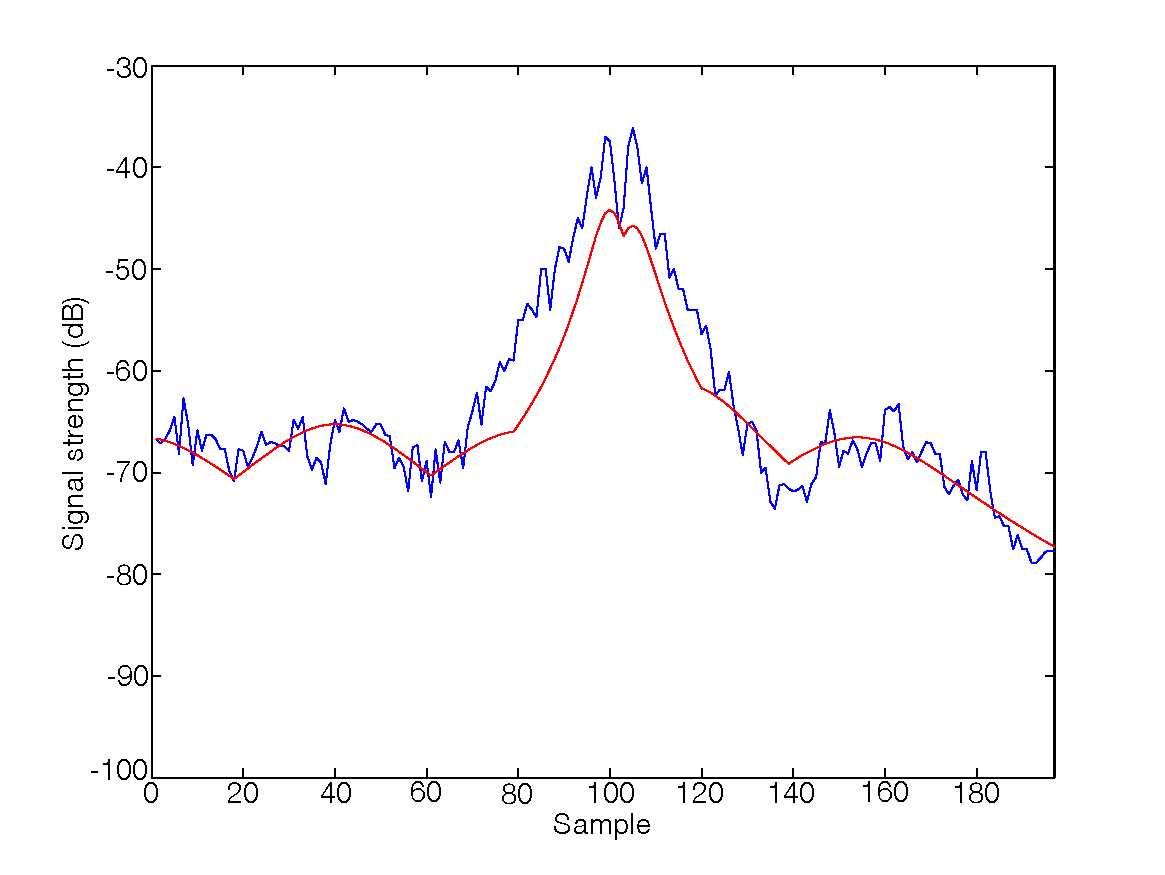
\includegraphics[width=1\textwidth ]{images/signal_model/log_norm_n_3_2}
\caption{Measured signal strength (blue) versus signal strength modeled using the log-normal shadowing model with $n=3.2$ (red).}\label{log_norm_n_3_2}
\end{figure}
%
\begin{figure}[!hbt]
\include{graphics}
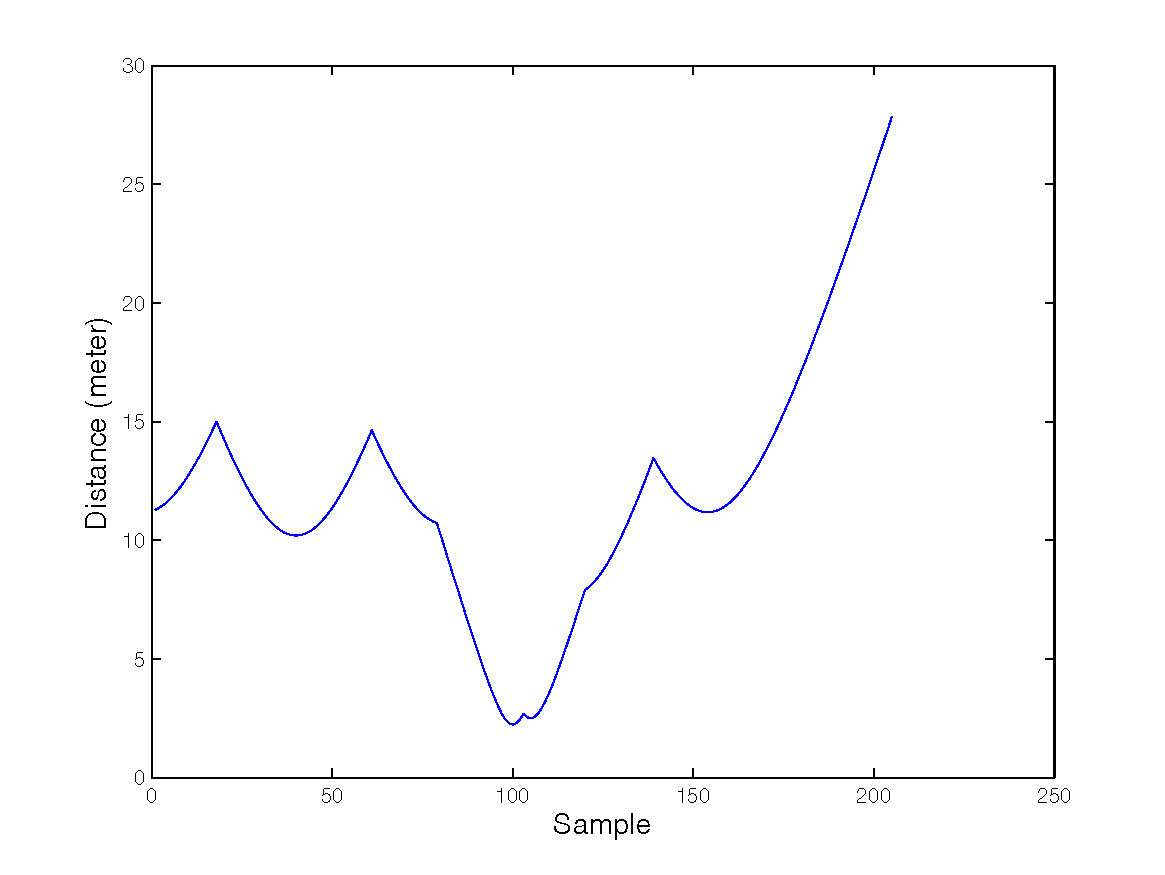
\includegraphics[width=1\textwidth ]{images/signal_model/dist_trans}
\caption{The distance to the transmitting antenna in meters used in the measurements of the signal strength}\label{dist_trans}
\end{figure}

It is obvious that this model has its flaws. A low value of $n$ fails to predict good signal strengths when the distance to the transmitter is fairly large, and the high value does not perform satisfactory close to the transmitter. The measurement taken is similar to a real world use-case where one moves through an office space, sometimes under a transmitter in line-of-sight and sometimes being far away in an obstructed area. The flaws promote the search for a model with better performance.
%
\subsection{Double Slope Model}
%
A simple extension of the log-normal shadowing model is combining different values of $n$ for use in various intervals of the distance to the transmitter. The most simple of these models is the double slope model where two different path loss exponent $n_1$ and $n_2$ are used together with a single break distance $d_1$, where the model changes from one to the other. This model then becomes,
\begin{subequations}
\begin{align}
\log_{10}({P_r(d)})&=\log_{10}({P_r(d_0)})-10n_1\log_{10}\left[{\frac{d}{d_0}}\right] + X_{\sigma_1}, & d_0<d<d_1\\
\log_{10}({P_r(d)})&=\log_{10}({P_r(d_0)})-10n_2\log_{10}\left[{\frac{d}{d_0}}\right] + X_{\sigma_2}, & d>d_1
\end{align}
\end{subequations} 
where $X_{\sigma_1}$ and $X_{\sigma_2}$ are random Gaussian distributed variables with zero mean and standard deviation $\sigma_1$ and $\sigma_2$ respectively.
 
In Figure \ref{double_slope} the double slope model for $n_1=2$, $n_2=3.2$ and $d_1=10$ meter, is displayed together with measurements using the distance trajectory in Figure \ref{dist_trans}.
%
\begin{figure}[!hbt]
\include{graphics}
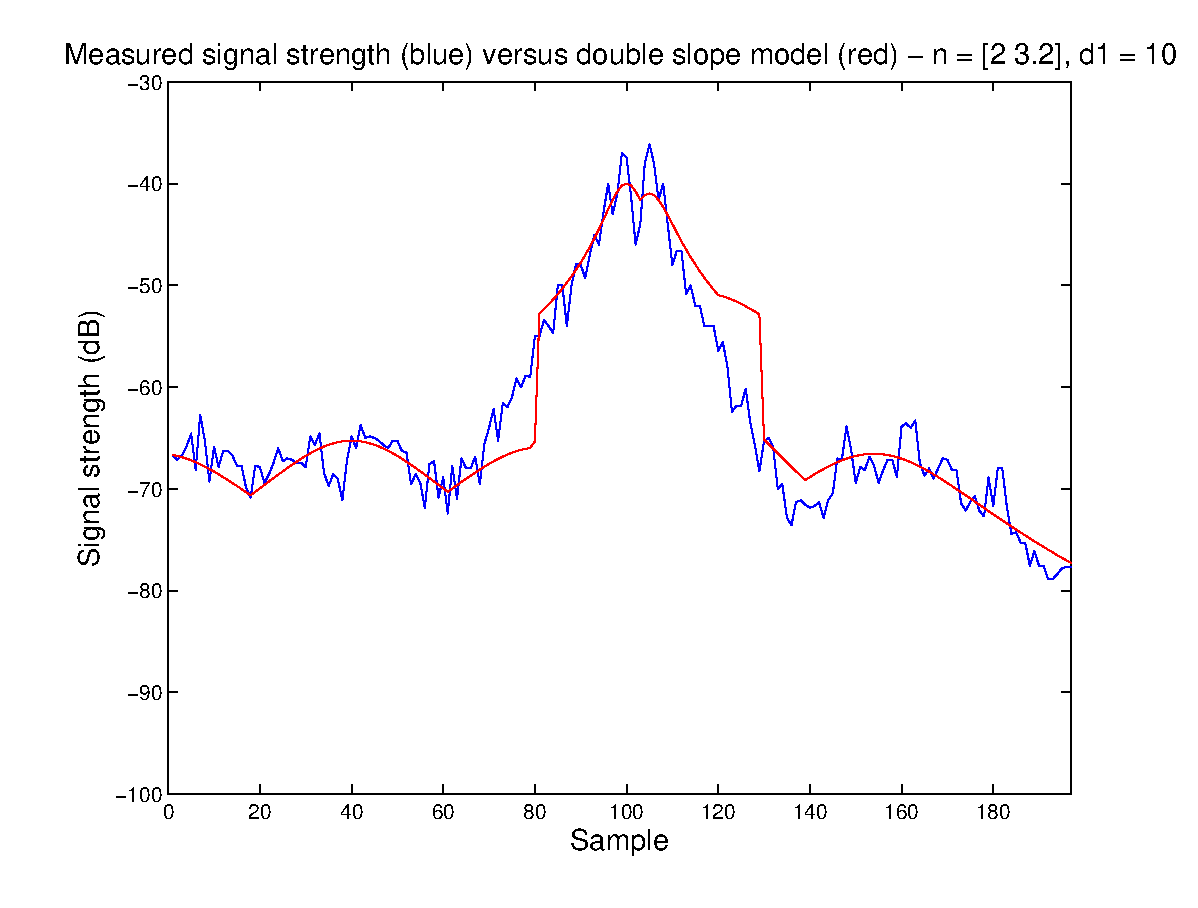
\includegraphics[width=1\textwidth ]{images/signal_model/double_slope}
\caption{Signal strength measurements (blue) versus double slope model predictions (red) with $n_1=2$, $n_2=3.2$ and $d_1=10$ meter.}\label{double_slope}
\end{figure}

This model combines the good traits from the two log-normal shadowing models. However, at $d=d_1$ the model presents an undesirable ''jump'', and the predictions around $d_1$ are rather poor. Furthermore, a single $d_1$ might be hard to find for a set of transmitters, and the different values of $n$ may change between the transmitters.
%
\subsection{$\alpha$-Model} %Maybe something else
%
A third attempt to model the signal strength is to introduce a parameter $\alpha$ multiplied with the distance $d$ in the log-normal shadowing model to account for the extra decrease in signal strength. \cite{karlsson92} The model then becomes
%
\begin{equation}
\log_{10}({P_r(d)})=\log_{10}({P_r(d_0)})-10n\log_{10}\left[{\frac{d}{d_0}}\right] - \alpha d+ X_\sigma.
\end{equation}
%
where $X_\sigma$ is a zero-mean Gaussian distributed random variable with standard deviation $\sigma$.

A typical choice of $n$ for indoor conditions is 2 or slightly less, to account for the LOS case when $d$ is small, see Table \ref{table:path_loss_n}. The range of $\alpha$ is around $[0.3,1.5]$, depending on the building.

This model possesses the desirable feature of having only one parameter, $\alpha$, to tune after the initial $n$ is chosen. However, it tends to underestimate the signal strength at large distances $d$, as $\alpha d$ grows linearly with $d$ while all other parts grow as the logarithm of $d$. Two simple ways to correct this easily comes to mind. Either the model can be changed to a log-normal shadowing when $d$ is large, or a maximum of $\alpha d $ may be imposed. The first of these becomes
%
\begin{subequations}
\begin{align}
\log_{10}({P_r(d)})&=\log_{10}({P_r(d_0)})-10n_1\log_{10}\left[{\frac{d}{d_0}}\right] -\alpha d+ X_{\sigma_1}, \hspace{2pt} d_0<d<d_1\\
\log_{10}({P_r(d)})&=\log_{10}({P_r(d_0)})-10n_2\log_{10}\left[{\frac{d}{d_0}}\right] + X_{\sigma_2}, \hspace{2pt} d>d_1
\end{align}
\end{subequations} 
and the second
\begin{equation}
\log_{10}({P_r(d)})=\log_{10}({P_r(d_0)})-10n\log_{10}\left[{\frac{d}{d_0}}\right] - \alpha*\min({d, d_{\text{max}})}+ X_\sigma.
\label{equation:fixed_alpha}
\end{equation}
%
Using one of these approaches, one loses some of the simplicity of having only one tunable parameter. However, these choices are simpler than for the double slope model, as there is no need to determine when the change from LOS occurs. 
For \ref{equation:fixed_alpha} the predicted signal strengths for $n=2$, $\alpha=0.9$ and $d_{\text{max}}=20$ are shown together with measurements in Figure \ref{fixed_alpha}. 
 %
 \begin{figure}[!hbt]
\include{graphics}
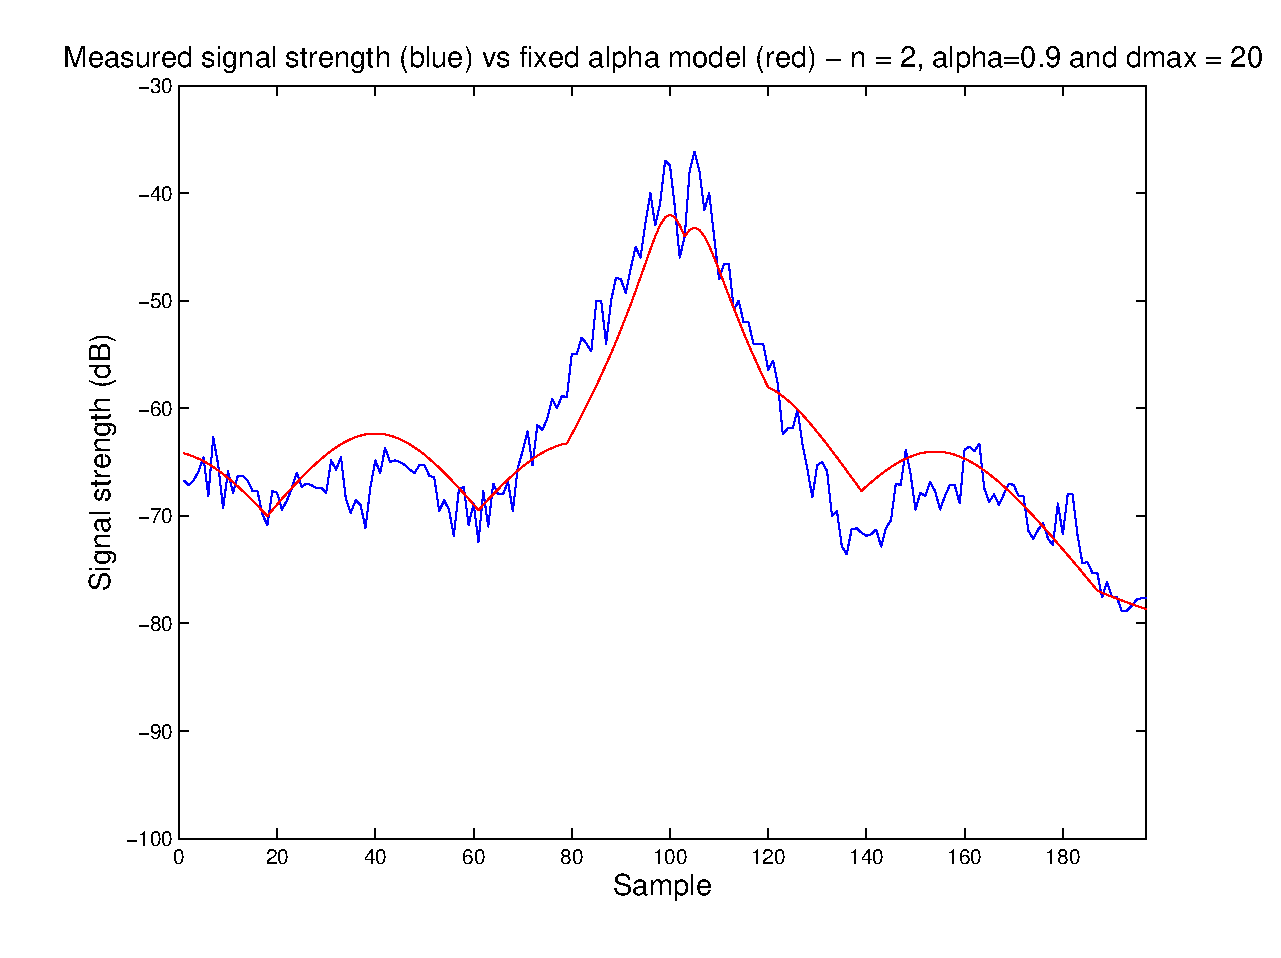
\includegraphics[width=1\textwidth ]{images/signal_model/fixed_alpha}
\caption{Signal strength measurements (blue) versus fixed $\alpha$ model predictions (red) with $n=2$, $\alpha=0.9$ and $d_{\text{max}}=20$ meter.}\label{fixed_alpha}
\end{figure}

This model predicts the signal strength satisfactory both for small and large values of $d$, while removing the ''jump'' present in the double slope model.
 %
 \section{Small Scale Fading}
 %
In addition to the large scale propagation effects described above, a radio signal usually displays a phenomenon called small scale fading. The small scale fading causes the signal strength to fluctuate rapidly over small distances or short time-spans \cite{rappaport96}. This effect is caused by different waves of the transmitted signal, called \emph{multipath waves}, arriving at the receiver with a slight time difference and thus causing interference. It can be a reflected or scattered wave arriving right after the direct wave, or reflected/scattered waves from different sources reaching the receiver at different times. 

Another effect included in small scale fading is a random frequency modulation caused by different Doppler shifts on different multipath signals. The source of this is a relative movement between transmitter and receiver or movement by objects in the vicinity of the signals path. 

The description presented above is brief, and for a more complete description of the small scale fading phenomenon readers are referred to chapter 4 in \cite{rappaport96}.  
 %
 \section{Aspects for Positioning Applications}
 \label{sec:AfPA}
 %
 For a signal strength model to be practical for positioning, it needs to possess two properties. It needs to predict the mean signal strength at a specific distance with satisfactory precision, and the variance around the mean should be sufficiently small. A few different approaches to reach this goal are available. One is to try to characterize the environment where the positioning is taking place, using measurements of the signal environment in numerous points. This is feasible only when the environment is fairly uniform, as the resulting model is an approximation for the entire environment. 
 
 Another approach is to create a signal strength map of the entire environment, by a large set of measurements. This is called \emph{fingerprinting}, and overcomes the problem of having a changing environment. However, it is impractical if used in a large area. 
 
 A third way of finding a model is to try to estimate the model parameters while the positioning is ongoing. This requires that at some point during the positioning, the position error is known to be small. Using this knowledge suitable model parameters can be calculated. Estimating the model has the advantaged of not being tied to a specific environment and whilst staying in the same environment the model will continue to improve. On the other hand it may not produce the best results, especially when moving between different environments or if small positioning errors are rare or hard to distinguish.        
 %
\chapter{The Particle Filter}
\label{chap:PF}
%
The \emph{particle filter} or \emph{sequential Monte Carlo methods} are sets of estimation algorithms for estimating the posterior density of the state-space in a non-linear filtering problem. The particle filter uses a set of particles distributed over the state-space using a system model and state measurements are used to determine each particle's probability to represent the ''true'' state of the system.  

In this chapter the non-linear filtering problem will be explained along with its solution using the particle filter. Some computational aspects will be investigated and the particle filter used in positioning briefly discussed. The chapter ends with a section about other estimation techniques, where most focus is placed on the \emph{least squares estimation}.
%
\section{Non-Linear Filtering Problem}
\label{sec:nlfp}
The non-linear filtering problem consists of estimating the states in a non-linear non-Gaussian model on the general form
%
\begin{subequations}
\label{equation:nonlinear_model}
\begin{align}
x_{k+1} &= f(x_k,u_k,v_k) \label{equation:nonlinear_model_first}\\
y_k&=h(x_k,u_k) + e_k
\label{equation:nonlinear_model_second}
\end{align}
\end{subequations} 
%
where $f$ and $h$ are arbitrary non-linear functions of the states $x_k$, inputs $u_k$ and process noise $v_k$, furthermore $y_k$ is the measurement at time $k$. The measurement noise $e_k$ and process noise $v_k$ are random processes with arbitrary probability density functions \cite{gson12}. 

There is a large collection of filtering methods solving this estimation problem in different ways with different restrictions. One of the most common is the \emph{Kalman filter}. This method is intuitive, simple and computationally effective. On the other hand, it suffers from requiring the functions $f$ and $h$ to be linear, and the probability density functions of the process $v_k$ and measurement noise $e_k$ to be zero-mean Gaussian. The \emph{extended Kalman} filter solves the problem of $f$ and $h$ being non-linear, but still assumes $v_k$ and $e_k$ to be zero-mean Gaussian noise. Further, both Kalman approaches require the posterior distribution of the states to be zero mean Gaussian.

Here we will instead focus on another filtering approach, the \emph{particle filter}, also called the \emph{Sequential Monte Carlo method}. This is a simulation based approach for solving the estimation problem \ref{equation:nonlinear_model}, only requiring the probability density function of $e_k$ and $v_k$ to be known \cite{gson12,fig_fra10}.  

The particle filter consists of a set of $N$ particles $\left\{x^i\right\}_{i=1}^N$, which represent different samples of states. These particles are used to create an approximation of the distribution $p(x_k|y_{1:k})$  of the states $x_k$ given the set of measurements $y_{1:k}$. The strength of the particle filter is that the distribution $p(x_k|y_{1:k})$ can be arbitrary. On the other hand, to provide the same particle density the number of particles grows by the power of the number of states. Hence, if you have 10 particles and one state, you need 100 particles to provide the same density for two dimensions. For three dimensions, you then need 1000 particles. This makes the particle filter suitable only when the number of states is relatively small.
%
\section{The Particle Filter Process}
\label{sec:PF_process}
%
The process of the particle filter consists of three separate steps \cite{gson12}, 
\begin{enumerate}
\item \emph{Weighting of particles}: using the measurements each particle is assigned a weight, corresponding to the likelihood of its states being the true ones.
\item \emph{Re-sampling}: From the existing $N$ particles, create $N$ new ones by a clever choice.
\item \emph{State update}: Using some trajectory of the states, update the states of each particle.
\end{enumerate}
%
\begin{figure}[!hbt]
\include{graphics}
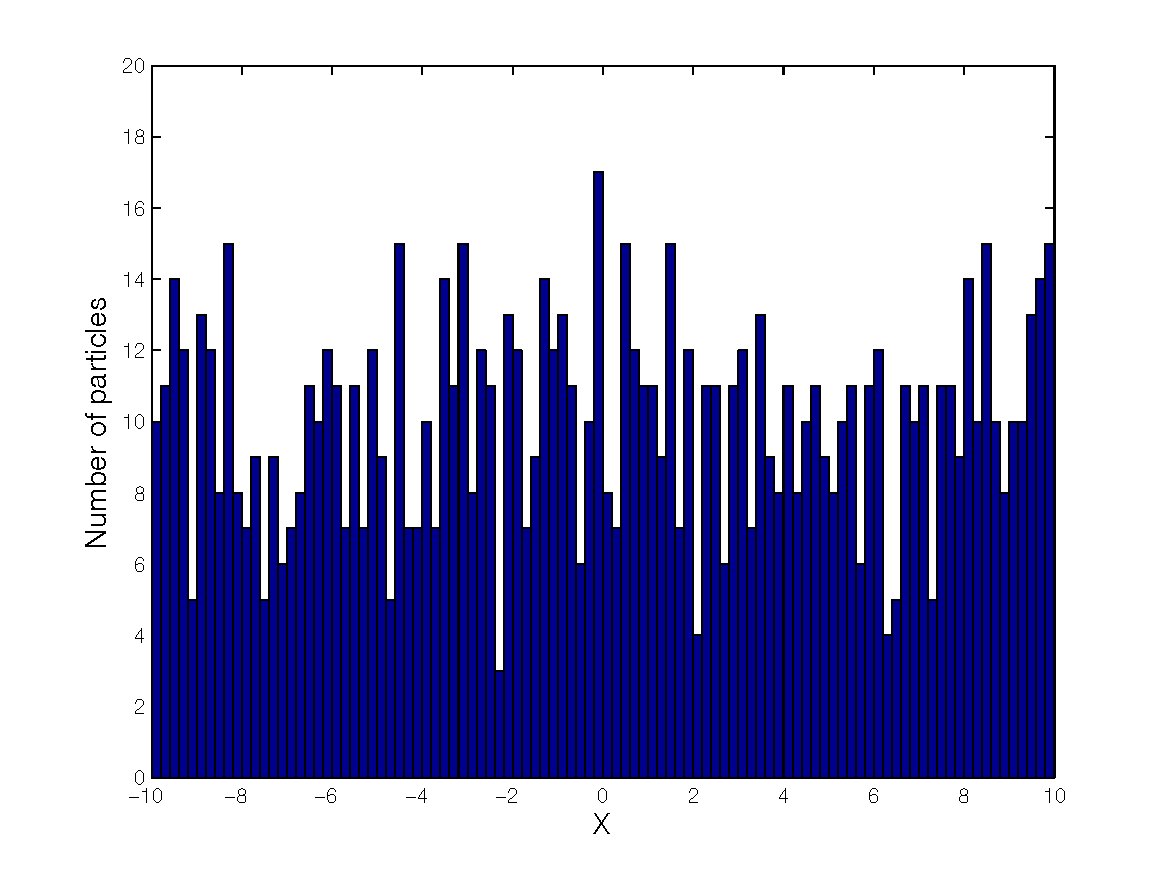
\includegraphics[width=1\textwidth ]{images/PF/hist_ini_dist}
\caption{Histogram over the initial particle distribution in range $[-10,10]$ using 100 bins}\label{hist_ini_dist}
\end{figure}
%
In the following sections these steps will be explored more in-depth along with a simple one dimensional example using $N=1000$ particles. We start by distributing the particles using a uniform distribution in the range $[-10,10]$, using $0$ as our true state and Gaussian distributed zero-mean random variable with standard deviation 1 as the measurement noise, $e_k$ from equation \ref{equation:nonlinear_model_second}. The initial particle distribution is displayed in Figure  \ref{hist_ini_dist}
%
\subsection{Computing the Weights}
%
Given that the measurement noise $e_k$ is known, the weighting of the particles is a straight forward process. For each measurement $y^l_{1:k}$ compute the probability $p^l(x^i_k|y^l_{1:k})$ that the particle $x^i$ has the true set of states. Then the total probability for each particle is,
%
\begin{equation}
p(x^i_k|y_k)=\prod_{l=1}^{L}p^l(x^i_k|y^l_{1:k}), 
\end{equation}
%
where $L$ is the number of measurements. It is also useful to have the probabilities satisfying,
%
\begin{equation}
\sum^{N}_{i=1}p(x^i_k|y_k)\equiv 1
\end{equation}
%
as to have the probabilities normalized.
%
\begin{figure}[!hbt]
\include{graphics}
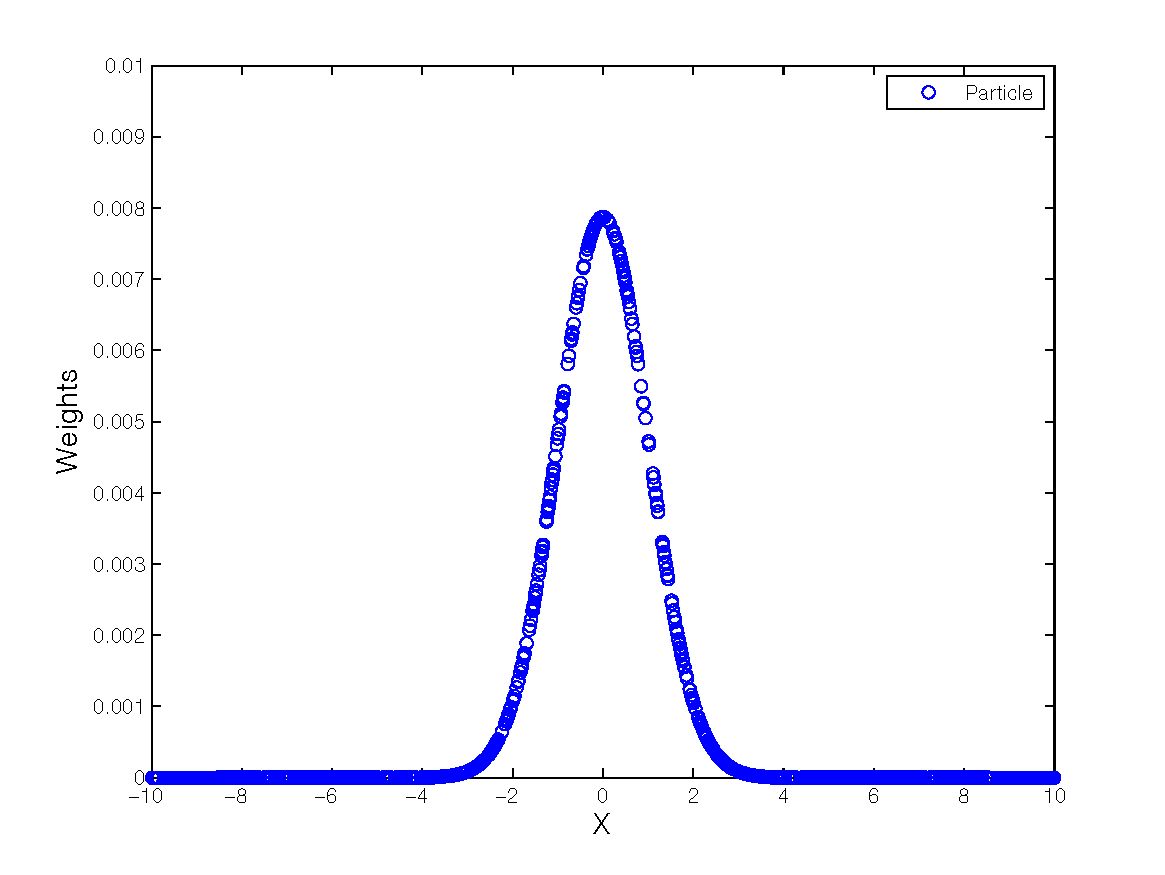
\includegraphics[width=1\textwidth ]{images/PF/particle_weights}
\caption{Particles versus their normalized weights.}\label{particle_weights}
\end{figure}

In Figure \ref{particle_weights} the normalized weights assigned to each particle in our example are displayed. It comes as no surprise that the weights resemble the normally distributed measurement noise. 
%
\subsection{Re-sampling}
%
The re-sampling step is introduced to eliminate the possibility of one or a few particles to be the only probable after a few iterations of the particle filter. If the re-sampling is omitted, the computing of weight and subsequent state update could dilute the particles in the state-space until only one particle is the probable one. This could be the case even if the most probable particle does not agree with the measurement. Thus, the purpose of the re-sampling is to use the weights to create $N$ new particles from the $N$ old ones. This can be done in many ways. One is to allow a number of the most probable particles to spawn new particles until $N$ particles are obtained. A statistically more stringent way is to compute a uniformly distributed random number $r$ between zero and one. Then, assuming the sum of all particle probabilities are one, start adding these until the sum is greater than $r$ Then, let the particle that caused the change spawn a new one. Using this method particles with high probabilities have a greater chance of spawning a new one, while particles with small weight still may create new ones.

After the re-sampling is done, it is crucial to give all particles the same weight, i.e $1/N$, as to avoid the dilution of probability.
%
\begin{figure}[!hbt]
\include{graphics}
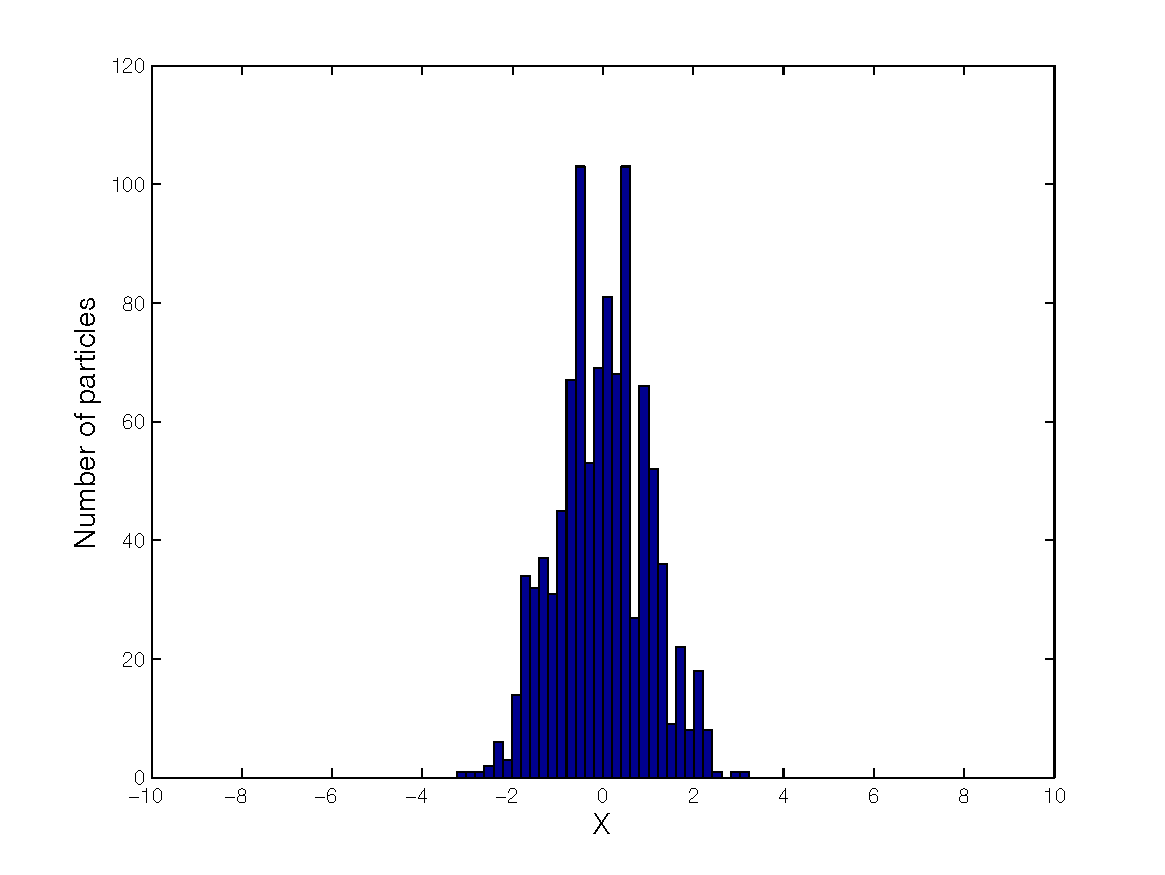
\includegraphics[width=1\textwidth ]{images/PF/hist_dist_1_itr}
\caption{Histogram over the particle distribution, after one iteration of the particle filter, in range $[-10,10]$ using 100 bins}\label{hist_dist_1_itr}
\end{figure}

After the re-sampling technique described above is applied to the particles of our example, their distribution is displayed in Figure \ref{hist_dist_1_itr}. After the re-sampling the states of the particles still existing tend more towards the true one, $X=0$. The mean of the states may now be used as an estimation of the true state.    
% 
\subsection{State Update}
%
In the state update step some model of the system behavior, $f(x_k,u_k,v_k)$ in equation \ref{equation:nonlinear_model_first}, is used to update the states of each particle in each time step, $k$. If the system behavior is well known, for one or all of the states, the use  of an elaborate model improves the convergence rate of the particles and thus the estimation accuracy. This usually allows the use of fewer particles, since there is no need to move particles to improbable states.

However, if there is little or no knowledge of the states behavior some type of random walk update can be used, only trying to capture the variance of the state over a time step. If the variance is large, this calls for a large number of particles to keep the particle density for all probable states high. 
%
\begin{figure}[!hbt]
\include{graphics}
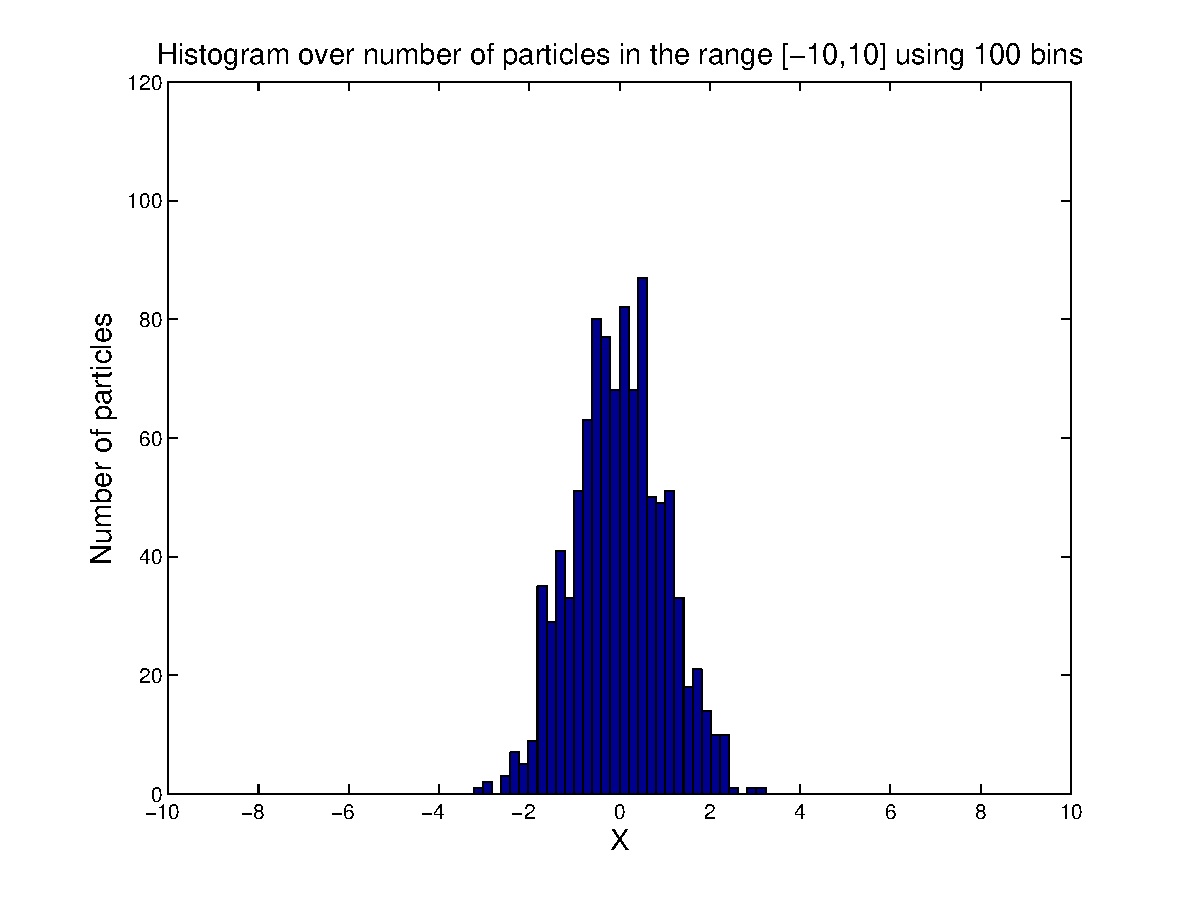
\includegraphics[width=1\textwidth ]{images/PF/hist_dist_1_itr_dyn}
\caption{Histogram over the particle distribution, after one iteration of the particle filter and a state update, in range $[-10,10]$ using 100 bins}\label{hist_dist_1_itr_dyn}
\end{figure}

In our example the ''true'' state is stationary, so the state update consists only of adding a Gaussian distributed random number with a small standard deviation ($0.1$) to each particle. This corresponds to letting each particle undergo \emph{Brownian motion}, and the resulting particle distribution may be viewed in Figure \ref{hist_dist_1_itr_dyn}.
%
\begin{figure}[!hbt]
\include{graphics}
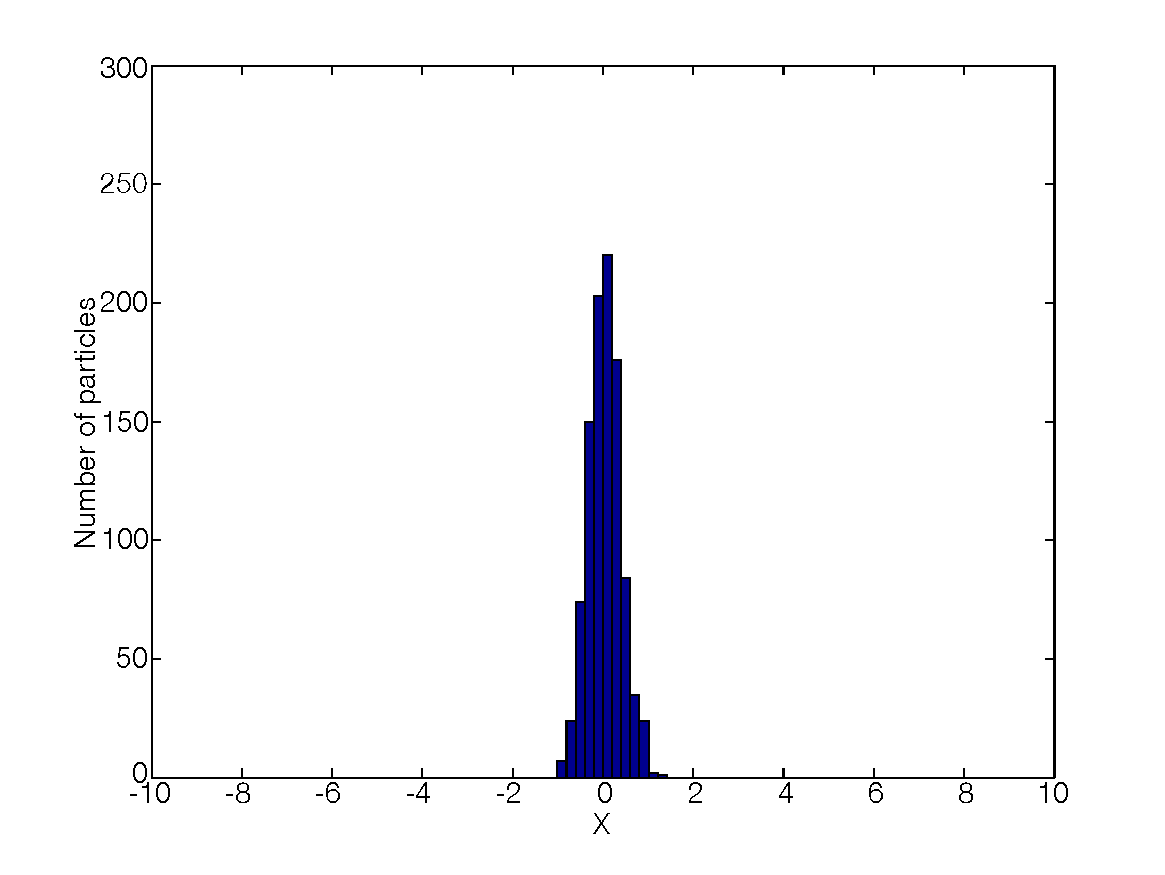
\includegraphics[width=1\textwidth ]{images/PF/hist_dist_10_itr}
\caption{Histogram over the particle distribution, after ten iterations of the particle filter, in range $[-10,10]$ using 100 bins}\label{hist_dist_10_itr}
\end{figure}

Finally, in Figure \ref{hist_dist_10_itr} the particle distribution after ten iterations is displayed, and the mean of the particle states is
\begin{equation}
\sum^{N}_{i=1}{\frac{x^i_{10}}{N}} = 0.04.
\end{equation} 
%
\section{Computational Aspects}
\label{sec:com_asp}
%
The particle filter, like most \emph{Monte Carlo} based filters, suffers from high computational complexity. Especially as the number of particles necessary to keep a fixed particle density in the state space grows as the power of the number of states. A solution to this is proposed in \cite{gson12}, where only states bearing non-linear distributions are passed throughout the particle filter and states bearing Gaussian distributions may be filtered by a different method. This is called the \emph{marginalized particle filter} and aim to keep the number of states passed to the particle filter low. 

The three steps discussed in section \ref{sec:PF_process} pose somewhat different computational difficulties. The weights need to be calculated for each particle and thus need to be computed $N$ times, giving an \emph{Ordo $N$} ($O(N)$) complexity. However, the calculation for each weight depends of the number of measurements $M$ giving a total complexity of $O(M*N)$. In most cases though, the number of measurements is small in comparison to the number of particles and may be neglected. Another pleasant feature of the weight computation is their independence of each other, thus making parallelization of computations simple.

The re-sampling step, assuming the number of samples before and after is constant, the algorithm described in section \ref{sec:PF_process} comprises two distinct steps. First the \emph{cumulative sum} of the weights are computed. This is of complexity $O(N)$ but can depending on the implementation be computed alongside the weights. Next, for the $N$ new particles, it is needed to determine which of the $N$ old ones is to be its clone. This is done by, for each new particle, computing a uniformly distributed random number in the range [0,1]. This random number is then compared to the cumulative sum of weights to find the index where the cumulative sum for the first time is equal to or larger than the random number. This can be done using a \emph{binary search} as the cumulative sum is sorted by its nature, giving the step complexity $O(N*\log_2{N})$. Furthermore, the particles are not entirely independent in this step, making parallelization cumbersome.

Updating the states is done for each particle and it depends on the number of states $K$ along with the complexity of the state model, resulting in roughly $O(N*K)$ complexity. During this step, the particles are entirely independent, which makes parallelization possible.

In all, the filter has approximately $O(N*\log_2{N})$, at least when the number of measurements $M$ and states $K$ are few compared to the number of particles.       
%
\section{Particle Filter for Positioning Applications}
%
The particle filter may be successfully used in positioning applications, especially if the states and models used possess certain features. More specific, the particle filter may be used with good results if the models are non-linear and the posterior distributions are non-Gaussian while the number of states is small \cite{gson12}. If the number of states grows, the ''curse'' of dimensionality makes the use the particle filter infeasible.

A case where the particle filter is useful is the estimation of position or position and heading in a two-dimensional space, which is the case for most indoor positioning applications. Furthermore, using signal strengths from multiple sources as a measurement of position renders, both a non-linear model and non-Gaussian posterior distributions further promote the use of a particle filter. However, introducing more dynamic states ,e.g acceleration, unmeasured velocities or trying to filter sensor biases or drifts, introduces too many dimensions. Thus, such estimations require their own filter \cite{gson12}.        
%
\section{Other Estimation Techniques}
\label{sec:oet}
%
There are a few different techniques for state estimation given a set of measurements, the \emph{Kalman} methods mentioned earlier, a couple of \emph{maximum.-likelihood} base ones and the \emph{least squares estimation} methods. \cite{gson12}
%
 \subsection{Least Squares Estimation}
%
The method \emph{least squares} is a common estimation technique for overdetermined systems, and is based on minimizing the error between an observed value and a modeled one. 

Given a series of $n$ measurements, $z_i$ and $n$ models $f_i(x_k)$ of the $m$ states $x_k$. The goal of the least squares estimation is the find the minimum of
%
\begin{equation}
S = \sum_{i=1}^n(z_i-f_i(x_k))^2
\label{ls_sum}
\end{equation}
%
given $n>m$. In the case of $f_i(x_k)$ being linear for all $i$, the algorithm is called the \emph{linear least squares} and $S$, in this case, has only one global minimum due to convexity. Also, an analytic solution is always present.

Generalizing the linear least squares estimation to non-linear models is fairly simple. The sum in \ref{ls_sum} is still to be minimized, but in the non-linear case a closed-form analytical solution can not be found. Instead the minimum is found by numerical approximations. As $S$ in the non-linear case is not, in general, convex, there exist multiple local solutions to the minimization problem. This requires a guess of the approximate states to ''guide'' the algorithm to the correct solution, and if the guess is too far from the global minimum, a local minimum could be found instead.     

The non-linear least squares can be used to estimate a position in two dimensions from the models in Chapter \ref{chap:RSP}, together with measurements of signal
% Fråga Fredrik:
 strengths from at least three access points. 
%
\chapter{Introduction to WiFi} %Working title
%Citation needed
The \emph{WiFi Alliance} defines WiFi as any ''wireless local area network (WLAN) products that are based on the \emph{Institute of Electrical and Electronics Engineers} (IEEE) $802.11$ standards''. However, since most WLAN products use the $802.11$ standards, in common tongue, WiFi and WLAN are interchangeable.    

This chapter is intended to give an introduction to the WiFi technologies and why these are of interest for indoor positioning.
%
\section{The $802.11$ Standard}
%
The IEEE $802.11$ standard consists of a series of techniques for over-the-air radio modulation using the same basic protocol \cite{IEEE:802.11}. The standard allows different products, computers, smart-phones etc. to implement the protocol to communicate wirelessly. Historically the communication has taken place over the frequency 2.4 GHz, however in later years devices implementing 5 GHz communication protocol have become increasingly common \cite{walrand10}.

The standard splits each frequency range into several channels over which the communication takes place. The frequency 2.4 GHz is split into 14 channels with 5 MHz spacing. For 5 GHz the situation is more complicated and will not be explained in detail. Local regulations affects which channels are allowed in a certain region.   

Wireless technologies are evolving towards higher frequencies. The radio channel  surrounding 2.4 GHz is well populated and a move to other frequency domains is necessary to continue to the technology expansion. Further, a near to full frequency environment promotes high noise levels and dropped connections due to interference between devices. Another advantage with transmitting information over a radio channel at a higher frequency is that the signal can contain more information per time unit, resulting in higher bit rates.    
%
\subsection{The MAC-Address}
%
Most devices using the IEEE $802.11$ standard have a \emph{Media Access Control} (MAC) address assigned as its network address \cite{IEEE:802.11}. The MAC address is usually assigned by the manufacturer and can be considered unique in a local area network. The address consists of twelve hexadecimal numbers. In its human readable form it is presented as six groups of two hexadecimal numbers, separated with either \verb|:| or \verb|-|, e.g. \verb|0a:1b:2c:3d:4e:5f|. They can be used to identify from which devices a signal originates.
%
\section{WiFi and Positioning}
%
The WiFi standard provides enticing possibilities for indoor positioning, especially in public or corporate areas. Some of the advantages compared to other positioning techniques is that the range of typical wireless products, like WiFi access points (AP:s), have limited range ($\sim 30$ meters) and thus need to be placed with relatively short intervals. Moreover, WiFi infrastructure is ubiquitous and already deployed at many places, making WiFi based positioning an attractive method. Further, more and more devices become capable of communication over WiFi and platforms like Android makes the deployment of applications easy and readily available for large amount of users. One of the disadvantages is that indoor signal environments are often complex, posing a harder modeling task and often rather high signal to noise ratio.

A few different techniques for indoor positioning are presented below.
%
\begin{itemize}
\item \emph{MAC-Address}:  

Receiving a signal, and thereby a MAC-address from an AP, indicates that the receiving device is within approximately $30$ meters, depending on building, transmitted power and effectivity of the receiving antenna. This is a rather crude positioning, but may be used to pinpoint a device to a certain area. Furthermore, receiving signals from multiple devices will improve the positioning, if the transmitter locations are different i.e reducing the possible position to a subsection of the area. 
%
\item \emph{Received Signal Strength (RSS)}:

Measuring the signal strength from an AP puts the devices not just in the vicinity, but gives a rough indication of the distance to the AP. Multiple APs may then be used to triangulate a position, but noisy measurements give a rather large uncertainty. 
%
\item \emph{Time of Arrival (ToA)}:

If the APs and measuring device are synchronized in time, the time difference between when a message was sent and received may be used to compute the distances between the device and the APs. However, the time differences involved are usually very short ($\sim 3*10^{-9}$ seconds per meter), especially in indoor environments, requiring the time synchronization to be precise.  
%
\item \emph{Round Trip Time (RTT)}: 

A way to eliminate the requirement of synchronized APs, is to measure the time it takes for a message travel to the AP and back again. This time is called the \emph{round trip time}. As only one device performs the time measurement the need for synchronization is eliminated, but instead the time from when an AP receives a message until it sends the response has to be known.
%
\end{itemize}
%
The techniques presented here assume that the measuring device is also performing the positioning. Similar approaches are available using the APs, to position devices in the environment. Furthermore, the technologies above could be combined or used together with different technologies such as Bluetooth, NFC, rfid etc. to increase the positioning accuracy. 
In this thesis however, the focus will be placed on the received signal strength.
%
\subsection{Received Signal Strength Indication}
%
The \emph{Received Signal Strength Indication} (RSSI) is a value indicating the short-time-average of the received signal power \cite{fig_fra10}. The RSSI is given in an arbitrary unit, but usually dBm, and there is no standard of how RSSI should be related to the physical properties of the received signal. This means different manufacturers of devices able to communicate over Wi-Fi may choose the range in which the RSSI is presented. 

For the RSSI to be a meaningful measurement of the received signal strength it must somehow be related to the physical properties of the signal. Usually, a measurement of the RSSI at a known distance is used together with an investigation of how the RSSI changes with the distance. The models discussed in chapter \ref{chap:RSP} can then be applied. Different devices may posses different parameters, thus requiring modeling for a specific device or an adaptive estimation scheme. 
%

\subsection{RSSI Measurements in Android}

An RSSI measurement on a device running the Android operating system is initiated by an application requesting a scan of the signal environment. The operating system performs the scan when the necessary system resources are available. Each channel specified by the IEEE $802.11$ standard and available in the current region is scanned. When a transmitter is found, a short-time average of the received signal power is measured and converted to an appropriate RSSI. The process is repeated until all reachable transmitters have been measured, and the results are returned along with information about each transmitter's MAC-address, its transmission frequency and a time-stamp. 

To conserve battery life for the measuring device, a technique called \emph{passive scanning} is used. Simply explained, each AP sends a message approximately every 100 ms telling devices in the vicinity it is active, its MAC-address and some additional information. The measuring device scans each channel for a little more than 100 ms to catch all APs on that channel, resulting in a quite long scan time ($\sim 3$-$5$ s), depending on the number of channels to be scanned. Most commonly the channels related to 2.4 GHz will be scanned first and subsequently the 5 GHz channels. This will generally introduce a time difference between the two different frequency measurements from a single access point.

Which channels to scan could be specified to reduce the scan time, but some AP data might then be lost. Another way of performing the scans is to have the measuring device actively probing (''asking'') for APs in its surroundings, but this would require almost constant sending of messages and listening for replies, thus draining the battery.               
%
\section{Performance of 2.4 GHz Versus 5 GHz}
%
The evolution of WiFi has prompted many AP:s to implement standards for both 2.4 and 5 GHz communications. Alongside the performance boost to devices able to use both frequencies, this poses an enticing possibility for higher performing indoor positioning. Different frequencies may, in the best case, provide two independent measurements of the distance to an AP. To investigate if this is the case, the correlation between the two frequencies must be determined.  
%
\subsection{Signal Correlation}
%
Of course, some of the signal behavior is expected to be highly correlated. For one, the large scale distance dependent path loss is largely the same in both signals, and it is from this path loss the distance to the AP is determined. Nevertheless, independence is a desirable feature for the signal noise, which includes the \emph{small scale fading}. 

To investigate the correlation between 2.4 and 5 GHz signals, measurements could be taken, with an increasing distance, to an AP transmitting on both frequencies. After the path loss dependent behavior is removed from the signals, the correlation of the noise could be computed. This process is illustrated for one series of data in Figure \ref{noise_corr_los} 
%
\begin{figure}[!hbt]
\include{graphics}
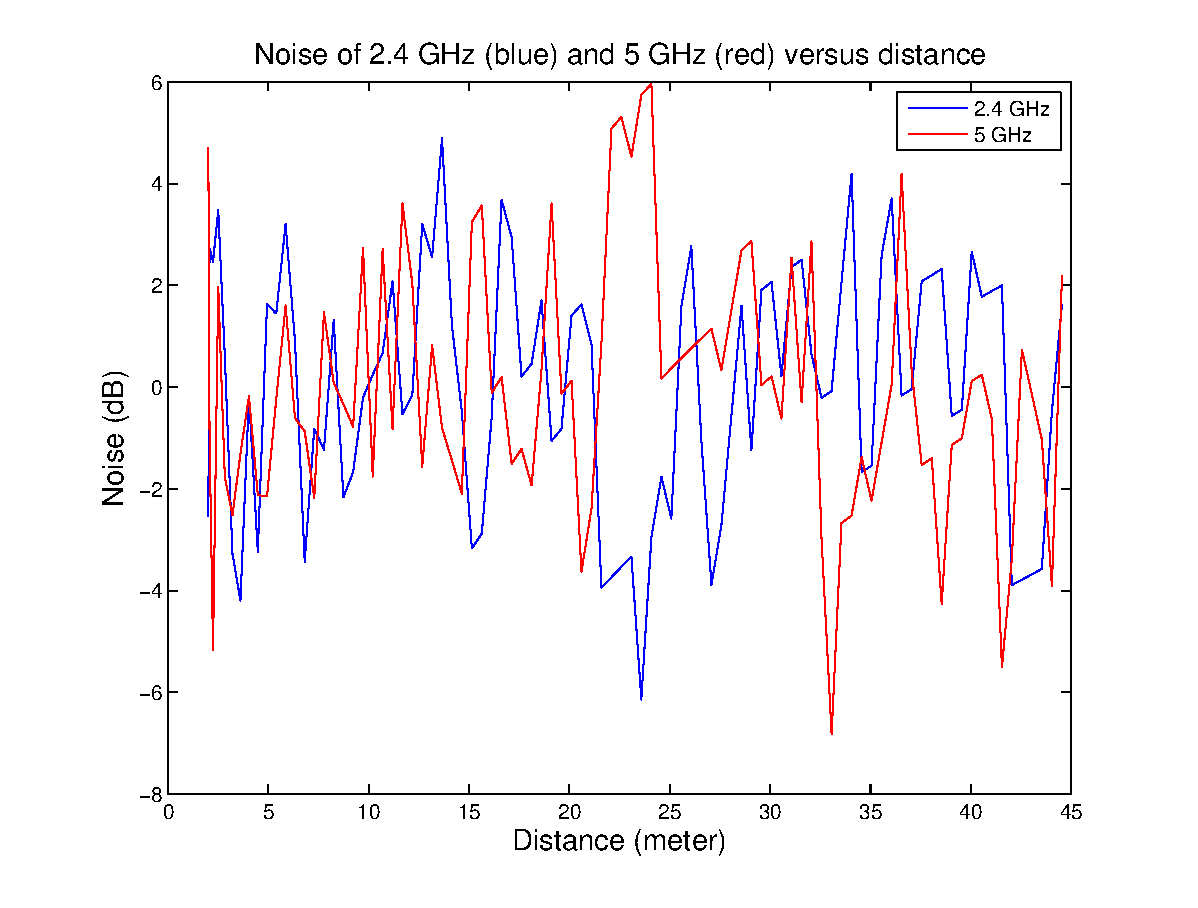
\includegraphics[width=1\textwidth ]{images/wifi/noise_corr_los}
\caption{Signal power, signal power together with linear trend and signal power minus linear trend for the 2.4 and 5 GHz channel. Measurements taken while traversing a distance of 15 meters, moving away from the AP.}\label{noise_corr_los}
\end{figure}

The \emph{correlation coefficient $\hat  r_{xy}$} between the two can be estimated using,
\begin{equation}
\hat r_{xy}=\frac{\sum\limits_{i=1}^{N}{(x_i-\bar{x})(y_i-\bar{y})}}{(N-1)\sigma_x\sigma_y},
\end{equation}
where $N$ is the number of measurements, $x_i$ and $y_i$ are the 2.4 and 5 GHz measurements compensated for the path loss, $\bar x$ and $\bar y$ their means and $\sigma_x$ and $\sigma_y$ their standard deviations. 

To construct a confidence interval for the covariance some statistic processing of the data is required. This presentation will be brief, and interested readers are referred to \cite{fisher15, fisher21}  for a more in-depth description. 

Since the distribution of $\hat r_xy$ is not Gaussian, \emph{Fisher's z-tranform}
%
\begin{equation}
z'=\frac{1}{2}\ln{\left(\frac{1+\hat r_{xy}}{1-\hat r_{xy}}\right)}
\end{equation}
%
is used. Under the current conditions, $ z'$ is normally distributed with standard deviation
%
\begin{equation}
\sigma_{z'}=\frac{1}{\sqrt{N-3}}.
\end{equation} 
%
The two-sided confidence interval for $z'$ at level $\alpha$ is then
%
\begin{equation}
I_{\hat z'} = \hat z' \pm Z_{\alpha/2}\cdot\frac{1}{\sqrt{N-3}}, 
\end{equation}
%
and may be transformed back to $\hat  r_{xy}$ using the \emph{inverse Fisher's z-transform},
%
\begin{equation}
\hat r_{xy}=\frac{e^{2z'}-1}{e^{2z'}+1}.
\end{equation}

In Table \ref{corr_conf} six estimations of the correlation between the noise of the 2.4 and 5 GHz RSSI measurements are presented. Four of these are estimated from data where the distance varies by 15 meters to the AP. Two of these are taken in LOS and two in NLOS, and for each case one measurement is taken near the AP and one far from the AP. The other two sets of data are taken at stationary positions in LOS and NLOS respectively.

The table shows that the correlations are significantly different from zero in some cases. At the same time, they are small with high probabilities. This means that additional information is added by using both frequencies, compared to using only one of them. It also means that the impact of the noise from one frequency can be reduced by using the other frequency as well.

However, the model errors, i.e. the difference between models and measurements, are still highly correlated between the frequencies. For example, if the user moves from LOS with an AP to NLOS, e.g. to the other side of a wall, both signal frequencies will be reduced in similar ways. Events like these are not modeled accurately, since one can not know when they occur. The result is a large correlation between the model errors for each frequency.
%
\begin{table}
\begin{center}
\begin{tabular}{|l|c|c|}
\hline
Signal path & Estimated covariance, $r_{xy}$ & 95 \% confidence interval \\
\hline
\hline
LOS near AP& -0.1039 & $[-0.2898;0.0896]$ \\
\hline
NLOS near AP& 0.2558 & $[0.0477;0.4426]$  \\
\hline
LOS far from AP& 0.2604 & $[-0.0853;0.5501]$\\
\hline
NLOS far from AP& 0.2364& $[0.0399; 0.4154]$ \\
\hline
LOS stationary  &-0.0644 & $[-0.1341;0.0060]$ \\
\hline
NLOS stationary  & -0.1191 &$[-0.1754;-0.0620]$ \\
\hline
\end{tabular}
\end{center}
\caption{Estimated covariances and 95 \% confidence interval for 2.4 and 5 GHz in different environments.}\label{corr_conf}
\end{table}
%
\subsection{Difference in Modeling}
%
An extensive discussion about how path loss depends on the frequency is done in \cite{rappaport96}, the gist of which is that higher frequencies lose power faster with distance. The difference between the behavior  2.4 and 5 GHz is not large (a factor $\sim 2$), however some extra attention is needed to model the two. To extend the models in chapter \ref{chap:RSP} to the difference in frequency, usually different $n$ or $\alpha$, depending on the choice of model, will be needed. Furthermore, an AP may transmit 5 GHz with a greater power than 2.4 GHz to mitigate some of the increased path loss, requiring measurements of the transmitted power for both frequencies.  
%
\chapter{Indoor Positioning - Pure RSSI Approach}
\label{chap:pure_rssi}
%
The signal propagation models described in Chapter \ref{chap:RSP} in combination with the particle filter from Chapter \ref{chap:PF} provides a framework for indoor positioning. This framework can be used to perform position estimation using RSSI measurements from multiple WiFi APs. 

In this chapter, the considerations about, and parameter choices for, the particle filter in the context of indoor positioning are presented. The performance is then tested in a few different environments and compared to position estimation using a \emph{least squares} algorithm.  These tests then serves as a basis for an extensive error analysis, discussing the error behavior depending on different conditions. The resulting knowledge is then used in the next chapter, to ascertain if and how adaptive or crowd-sourced signal strength models may be used.
%
\subsection{Importance of Geometry}
%
\begin{figure}[!hbt]
\include{graphics}
\includegraphics[width=1\textwidth ]{images/pure_rssi/geometries}
\caption{Probable positions for different access point configuration (\emph{white} \texttt{+}). \emph{Red} implies high probability and \emph{blue} low probability. The \emph{true} position is $[0, 20]$.}\label{geometries}
\end{figure}
%
How the access points are positioned in relation to the user (i.e. the position of interest to estimate), highly impacts the quality of the estimation. In Figure \ref{geometries}, three different AP geometries are shown along with the distribution of probable positions. It represents an idealized case where the noise in the measurements of the distance to each AP is zero-mean Gaussian. However, it provides an illustrating example of how the geometry impacts the distribution of the estimated position.

In the leftmost case in Figure \ref{geometries} the APs are placed on a straight line, and in this case trilateration of the \emph{true} position, $[0,20]$, is impossible if no prior information is known. As the figure shows, APs positioned on a straight line gives two equally probable position estimates (more \emph{red} implies higher probability), i.e. it is not possible to distinguish between a position and its mirror image in the line formed by the APs. 

The second case displays a scenario where the APs are placed in the corners of a obtuse triangle (largest angle greater than $90^\circ$). In this rather ideal case it is possible to discern the \emph{true} position as the most probable one. However, higher noise levels and/or biased noise in the measurements will make this increasingly hard, as there are two different positions with relatively high probabilities.

The third case represents a best-case scenario where the position to be estimated is centered in an equilateral triangle. Here, it is easy to distinguish the most probable position, and likewise the \emph{true} position.

The particle filter uses information about the positions at previous time steps making it more likely to determine the true position even if the current geometry is disadvantageous. The least squares estimation, on the other hand, uses only instantaneous measurements and will suffer much more severely from a unfavorable environment. 
 
The positioning will further benefit from a larger number of APs as both the number of measurements and the probability of having an advantageous geometry increase. Still, a few conclusions could be drawn from this discussion, the main one being that measurements are taken inside a polygon with corners consisting of the APs tend to provide the best information about the true position regardless of the used estimation algorithm. 
%
\section{On Parameter Choices}
%
There are four parts of the particle filter that can be chosen by the user to some extent. The number of particles $N$, the system model, the process noise $v_k$ and the measurement noise $e_k$.
%
\subsection{System Model}
%
The process model is the most extensive choice, where both the number of states and their respective dynamics need to be determined. Some parts of this are dependent on available measurements and how complex the model is allowed to be. Using only measurements of the RSSI from multiple APs, a simple model using two states $x$ and $y$, describing the position in a plane, are used. Moreover, a random walk process is used to model the dynamics, resulting in the state update
%
\begin{eqnarray}
x_{k+1}&=x_k + v^x_{k+1} \\
y_{k+1}&=y_k + v^y_{k+1} 
\end{eqnarray}
%
where $v^x_k$ and $v^y_k$ are the process noise on each state. 
%
\subsection{Process Noise}  
%
The process noise is, in this case, rather straight forward to choose, as it represents the spread of particles in between measurements. A normal distribution around a circle with radius $r$ is an appropriate choice,
%
\begin{eqnarray}
v^x_k &\sim r\sin{\alpha_k}+N(0,\sigma^2)\\
v^y_k &\sim r\cos{\alpha_k}+N(0,\sigma^2)
\end{eqnarray}
%
where
%
\begin{equation}
\alpha_k \sim \mathsf U(0,2\pi).
\end{equation}
%
$\mathsf{U}(0,2\pi)$ is a uniform distribution between $0$ and $2\pi$. $\sigma$ is the standard deviation of the normal distribution. In this case $r$ is a approximation of how far the phone travels between two measurements and $\sigma$ measures the uncertainty of this distance. 

A fair estimation is that a walking person travels at between 1 and 2 meters per second, and given an interval $\Delta t$ between measurements it holds that $r \approx 1.5*\Delta t$ and $\sigma \approx 0.5*\Delta t$. Thus,
%
\begin{eqnarray}
v^x_k&\sim 1.5\Delta t \sin{\alpha_k} + N \left(0, \left(\frac{\Delta t}{2}\right)^2\right)\\
v^y_k&\sim 1.5\Delta t \cos{\alpha_k} + N \left(0, \left(\frac{\Delta t}{2}\right)^2\right)\\
\end{eqnarray}
places the new particles somewhere on a circle of radius $1.5\Delta t$ from the old one and spreads them by a standard deviation of $0.5\Delta t$.

This estimation could be further improved by the use of a technique for counting steps, and this approach will be investigated in later chapters.    
%
\subsection{Measurement Noise}
%
The measurement noise can be estimated in the following way. Take a set of RSSI measurements from a certain AP, and vary the distance. Then model a received RSSI at each distance and compute the noise as the difference between model and measurement. The standard deviation of measurement noise can then be estimated as the average of the absolute value of the noise. To estimate the noise accurately a large set of data in different environments is required.

This has been done for a quite large number of AP:s, and in environments ranging from LOS to a highly obstructed signal path. Some of these results are displayed in Figure \ref{noise_behaviour}. 
%
\begin{figure}[!hbt]
\include{graphics}
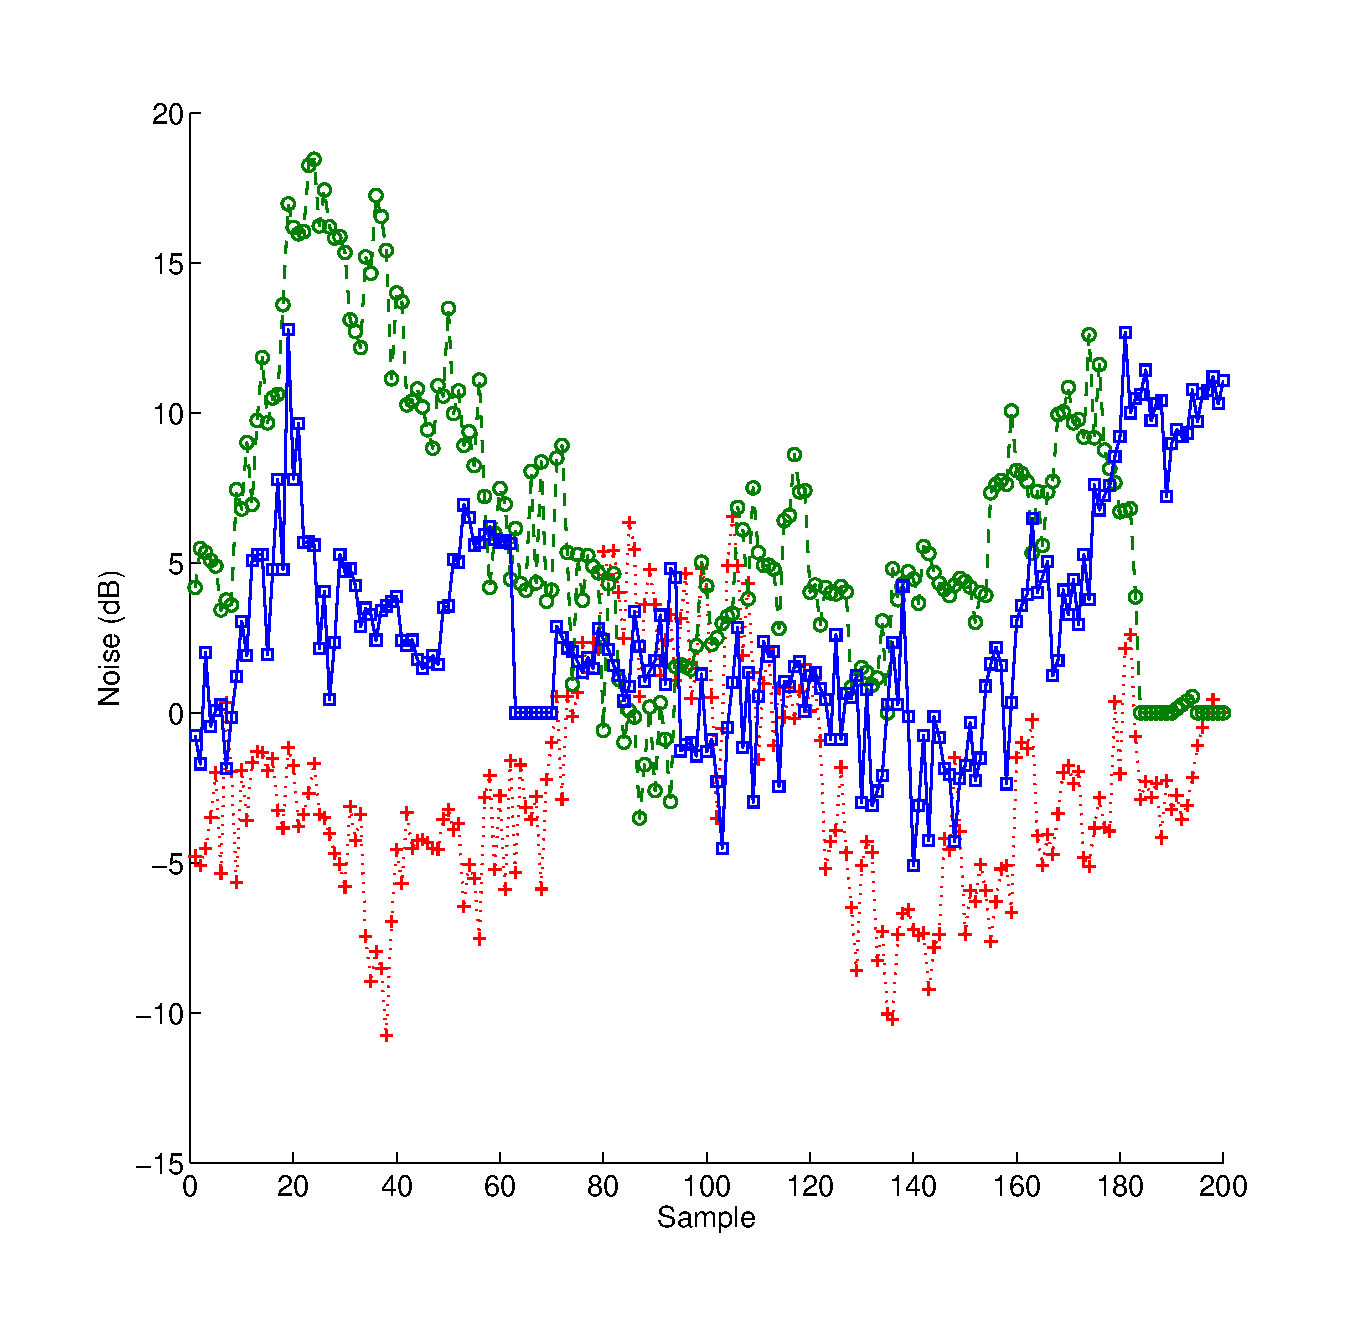
\includegraphics[width=1\textwidth ]{images/pure_rssi/noise_behaviour}
\caption{The difference between measurements and model for a few different APs for different environments and distances. Notice that the \emph{y}-axis of the figures are different.}\label{noise_behaviour}
\end{figure}

The resulting variance in the measurements ranged from $9$ to $60$, with a mean of $25$. The reason for the large span is that some of the APs were in LOS for most of the measurements even though the distance to them was fairly large. Other AP:s were, on the other hand, highly obstructed while at a quite short distance, and yet others followed the models well. 

During the position estimations in the rest of this chapter the mean of the variance, $25$, will be used. Further, the measurement noise will be assumed to be Gaussian with zero mean. This assumption is valid for data sets covering large distances. However, over a short traveled distance the noise is expected to be biased in some cases as it is highly dependent on the environment. This is somewhat mitigated by having measurements from numerous AP:s, allowing positive and negative biases to cancel.

\subsection{Number of Particles}
%
\begin{figure}[!hbt]
\include{graphics}
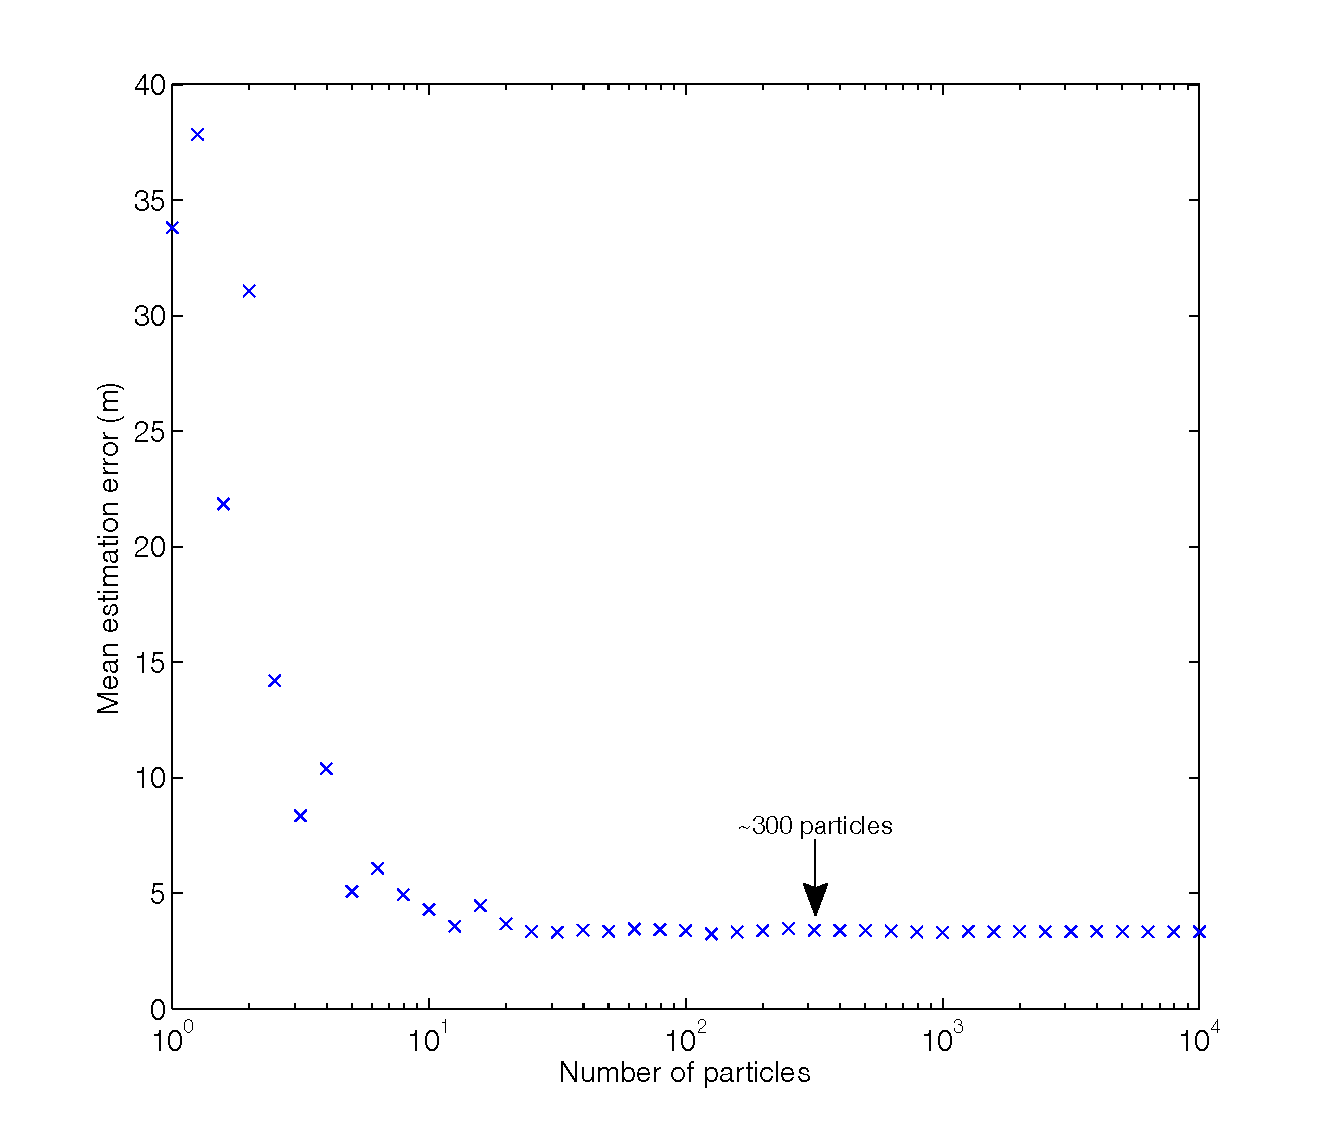
\includegraphics[width=1\textwidth ]{images/pure_rssi/err_vs_N}
\caption{Mean error in estimated position versus number of particles, $N$, for a two dimensional positioning.}\label{err_vs_N}
\end{figure}

The number of particles required to maintain a high enough distribution over the relevant part of the state space, is dependent on the size of the state space and the distance traveled in between filter updates. In this case, the size of the state space is two, position in x- and y-direction respective, as the positioning is done in two dimensions. The distance in between filter updates i.e distance between consecutive RSSI measurements changes for different test cases. The range starts at 0.5 meters with a close to zero variance, when measurements are taken every 0.5 meters around a predefined path. The other limit of the range is around 4 meters with considerably larger variance when measurements are taken around every third second while walking a predetermined path. 

In Figure \ref{err_vs_N}, the mean positioning error for the same data set is shown, for different numbers of particles, $N$, ranging from $1$ to 10 000. The data was generated by measurements taken with 3 meters of relative spacing along a predetermined path. For small $N$, the error improves dramatically when $N$ is increased. However, for $N$ larger than $\sim 40$ no further improvements are noticeable and the mean estimation error settles at $\sim 3.5$ meters. 

For some of the test cases used later in this chapter, the distance between measurements and its variance will be lower, and for others, considerably higher, compared to the case presented in the previous paragraph. To accommodate for this a larger $N$, of 300, is chosen and used for all tests in the following sections.    
%
\section{On model choice}
%
From chapter \ref{chap:RSP}, a model on the form
%
\begin{equation}
R_x(d) = C - 2*10\log_{10}{d}-\alpha d
\label{eq:RSSI_model}
\end{equation}
%
is determined appropriate to model the RSSI measurements. In this model, $R_x(d)$ is the RSSI measurement at a distance $d$ from the transmitter, $C$ is related to the power of the transmitter and $\alpha$ models path loss related to signal path obstruction. 

The models are discussed in chapter \ref{chap:RSP} but appropriate values of the constants $C$ and $\alpha$ are yet to be determined. This may be done in a couple of fashions, two of which will be presented here. The resulting values, especially the value of $\alpha$, are highly dependent on the environment, thus making them, in this situation, suitable for a open office environment. The values of $C$ is also related to the power with which the Wi-Fi access points transmits, so a different AP will most likely have a different value.      

\subsection{Model Driven Approach}
%
Given measurements at known locations, preferably with both obstructed and line of sight paths to the access points, it is possible to compute the model parameters.

The value of $\alpha$ from \ref{eq:RSSI_model} can be calculated as
%
\begin{equation}
\alpha = \frac{C-2*10\log_{10}(d)-R_x(d)}{d}.
\end{equation}
%
The estimation of $\alpha$ will improve if the paths between transmitters and receiver is representative for the desired environment.  

To find the value of $C$, measurements of the RSSI should be performed in line of sight of the AP, at different locations and with different distances to the AP. The value can then be calculated from
%
\begin{equation}
C=R_x(d) - 2*10\log_{10}(d)
\end{equation}
% 
i.e from \ref{eq:RSSI_model} with $\alpha = 0$ (line-of-sight).

This has been done at 20 different locations with 20 measurements of the RSSI from available APs taken at each. The estimated values of $\alpha$ and $C$ is presented in Table \ref{table:est_par}.

\begin{table}
\begin{center}
\begin{tabular}{|l|l|l|l|l|}
\hline
\multicolumn{1}{|c|}{Frequency, GHz} & $\alpha$ & $\sigma(\alpha)$ & $C$ & $\sigma(C)$ \\
\hline
\hline
2.4 & 0.332 & 0.319 & -40.7 & 2.97 \\
5.0 & 0.551 & 0.375 & -32.3 & 4.72  \\
\hline
\end{tabular}
\end{center}
\caption{Estimated model parameters and the standard deviation of the estimation, indicated by $\sigma$.}\label{table:est_par}
\end{table}
%
\subsection{Estimation Error Approach}
The other method is a bit more heuristic, but might produce equal or better performance. Instead of finding the values of $\alpha$ and $C$ by measurements it is possible to find the parameters resulting in the smallest average positioning error. This is done by taking a set of RSSI measurements at a few different known locations and use them in the position estimation algorithm with different $\alpha$ and $C$, to find the parameters producing the smallest mean estimation error.   

\begin{figure}[!hbt]
\include{graphics}
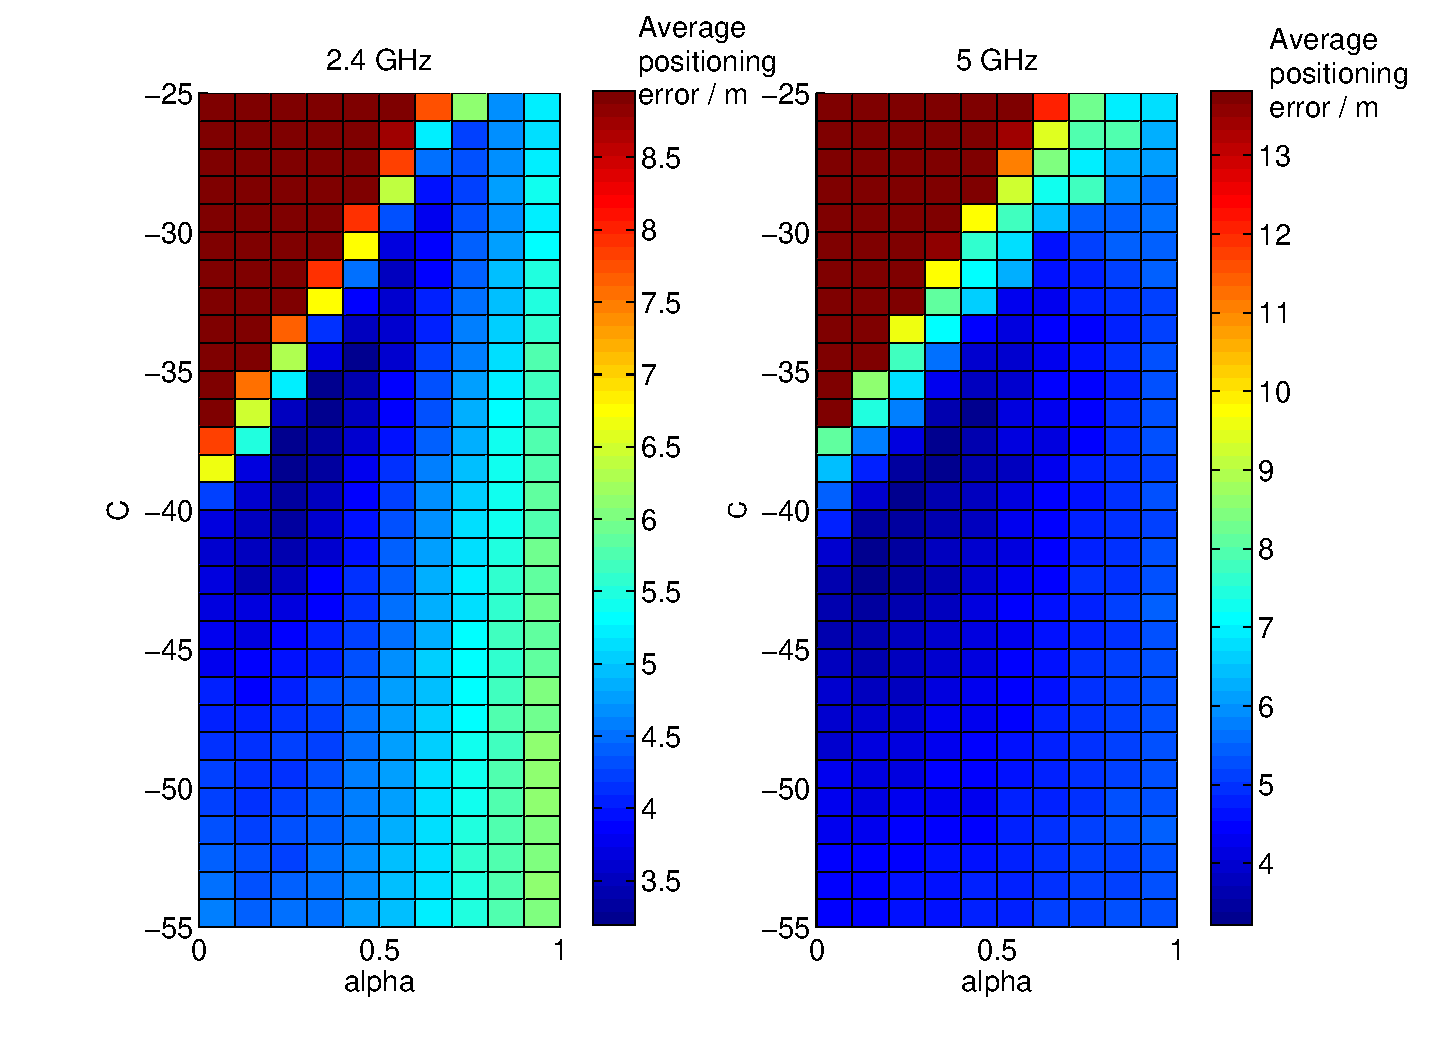
\includegraphics[width=1\textwidth ]{images/pure_rssi/err_vs_param}
\caption{Average estimation error as a function of $\alpha$ and $C$ for 2.4 and 5 GHz RSSI measurements. Values in deep blue (bottom left corner) are set to zero since these values resulted in very large positioning errors.}\label{err_vs_param}
\end{figure}
%
To illustrate this, the estimation error for $\alpha \in [0;1]$ and $C \in [-55;25]$ is shown in Figure \ref{err_vs_param} for 2.4 and 5 GHz. The parameters yielding the smallest average positioning errors is $C=-38$ and $\alpha = 0.3$ for 2.4 GHz and $C=-39$ and $\alpha = 0.2$ for 5 GHz. 
%
\subsection{Final Parameter Choice}
%
A few interesting observations can be made from the two methods above. The first of these being that the range of possible values are large, indicated by the standard deviations obtained from the model driven method. This is somewhat to be expected as the obstruction between transmitter and receiver is vastly different from location to location. Thus, the obtained parameters will be an average of the different environments giving rise to their high standard deviation. 

Further, it is noteworthy that the parameters obtained from the two approaches differ, especially for 5 GHz. One explanation for this is that the particle filter is able to find an accurate position given, for example, a positive model error for 2.4 GHz and a negative error for 5 GHz from the same AP. However, the parameters found trying to minimize the model error still produced small positioning errors when used together with the particle filter. 

Looking at Figure \ref{err_vs_param} the particle filter exhibits an interesting behavior. The positioning error is relatively small for a large range of parameters but a change to substantial errors happens suddenly for certain parameters. Parameter choices along the approximate line from $C=-25$ and $\alpha=0.7$ to $C=-39$ and $\alpha=0$ needs to be changed only by a small amount to produce either good or truly poor results. A deeper investigation shows that this line roughly translates to the models switching from estimating a too low signal power to estimating a too high one, for a certain location. The smallest positioning errors is obtained when the modeled and received power are about the same, placing them slightly above the line described earlier. However, these parameters are sensitive if the environment changes, resulting in estimating to high signal powers for the given location. A more robust choice is to over estimate the signal attenuation resulting in a higher $\alpha$. This choice might produce slightly larger positioning errors but is less sensitive to changing environments.

The conclusion of the discussion above is that it is far better to under estimate the signal power at a given location than to over estimate it. Taking this into account the values stated in Table \ref{table:model_par} will be used to model the received RSSI value at a distance, $d$ from the AP.  These values are more restrictive concerning the signal power than the parameters found previously. However, these choices provide a more robust estimation if the environmental properties change. The effect  of a small change in the true value of $C$, due to either variations in the power transmitted by the AP or different properties of the receiving device, will also be somewhat mitigated by a more restrictive choice of parameters.  
%
\begin{table}
\begin{center}
\begin{tabular}{|c|l|l|}
\hline
Frequency, GHz & $C$ & $\alpha$ \\
\hline
2.4 & -38 & 0.4 \\
\hline
5 & -36 & 0.5 \\
\hline
\end{tabular}
\end{center}
\caption{Model parameters for equation \ref{eq:RSSI_model}, to be used to model the RSSI for the following sections.}\label{table:model_par}
\end{table}
  
%
\section{Test Setup}
\label{sec:test_setup}
%
During the sections of this chapter two different test cases will be used,
\begin{description}
%
\item[Case 1:] \hfill \\
%
Measurements of the RSSI are taken at equally spaced points with $0.5$ meters spacing over a predetermined path. Only measurements from APs with known positions are used. The measurements are taken while the measuring phone is at rest at each point.  
%
\item[Case 2:] \hfill \\
%
Measurements of the RSSI is taken continuously while the user is walking a predetermined path at a relatively constant speed. The time between each measurement is approximately 4 seconds. Only measurements from APs with known positions are used.  
%
\end{description}
%
\emph{Case 1} allows the analysis of error between true position and estimated position as the measurements are taken at fixed points. Further, the distance between measurements can be changed in increments of 0.5 meters by using only a subset of the available data. 

\emph{Case 2} provides a more natural use-case, where the user is moving while trying to find his position. This case lacks the ability of error analysis, as the measurements are taken continuously over an interval and the time between two consecutive measurements is not fixed. However, the estimated trajectory can be compared to the true one.   

The tests were performed in a building called Glasgow, one of Sony's office buildings, on the 6:th floor. For different tests, different paths and a different setup of APs are used. Further, all tests are performed in the same type of open office environment, but the differences between the exact environments for each test are fairly large. During the tests, the user held the smart phone in one hand, with the screen pointing upwards. The smart phones used were one Togari and one Honami, both manufactured by Sony. These performed similarly except for a constant bias on the RSSI.
%
\section{Results}
\label{environment_results}
%
The results of the different tests performed are presented in the sections below. 
%
\subsection{Environment One - WORKING TITLE} 
%

%
\begin{figure}[!hbt]
\include{graphics}
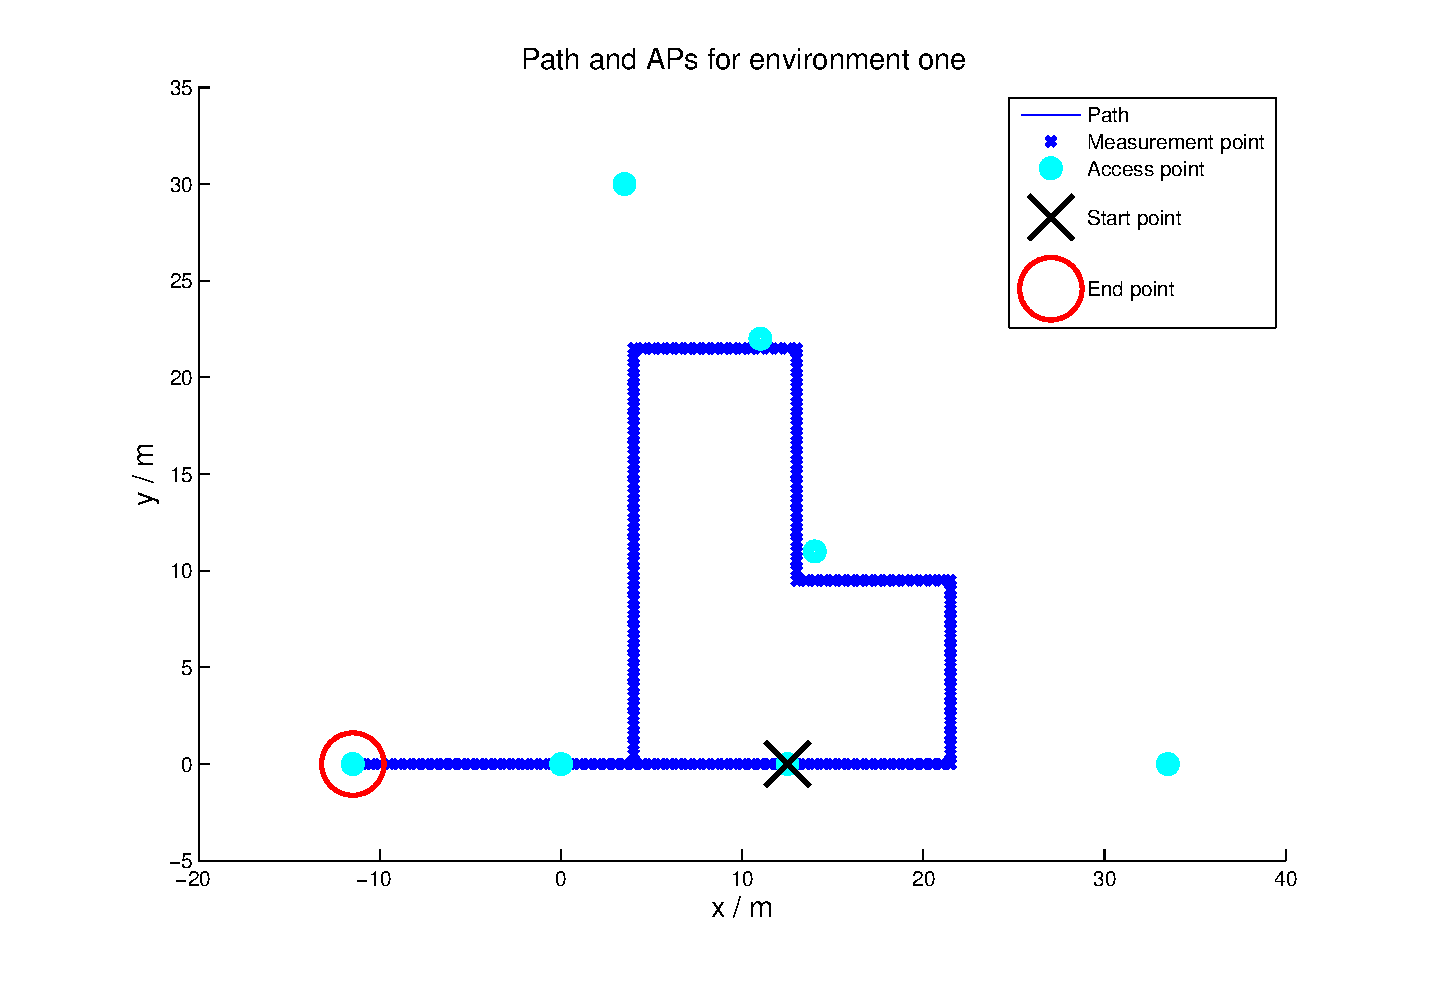
\includegraphics[width=1\textwidth ]{images/pure_rssi/env_one}
\caption{The path (\emph{blue} line) used in the \emph{environment one}, along with measurement points (\emph{blue} \texttt{x}), start point (\emph{black} \texttt{x}) and end point (\emph{red} \texttt{o}) }\label{env_one}
\end{figure}
%
\begin{figure}[!hbt]
\include{graphics}
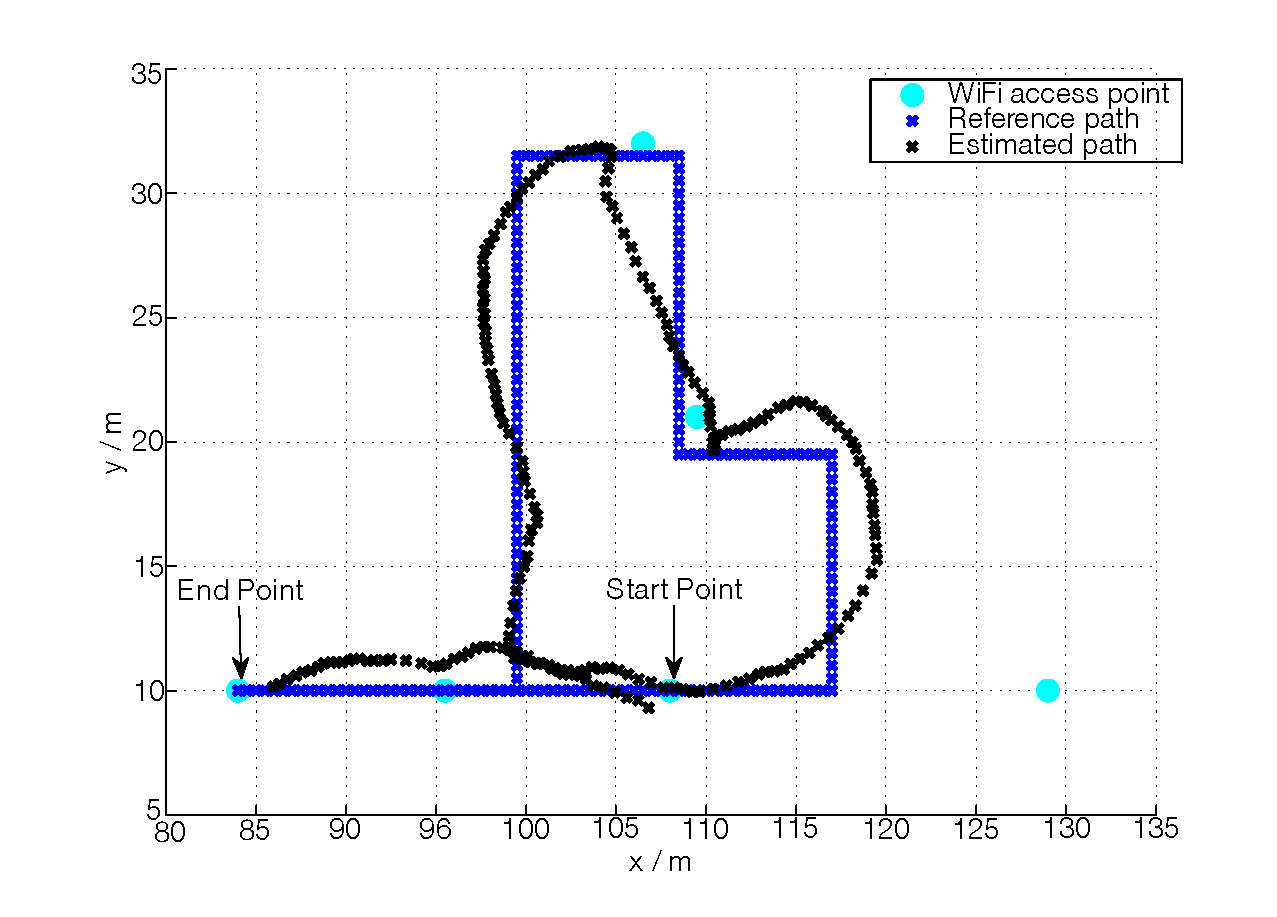
\includegraphics[width=1\textwidth ]{images/pure_rssi/true_vs_est_env_1_05}
\caption{Comparison between the true (\emph{blue}) and estimated (\emph{black}) path for \emph{environment one}.}\label{true_vs_est_env_1_05}
\end{figure}
%
\begin{figure}[!hbt]
\include{graphics}
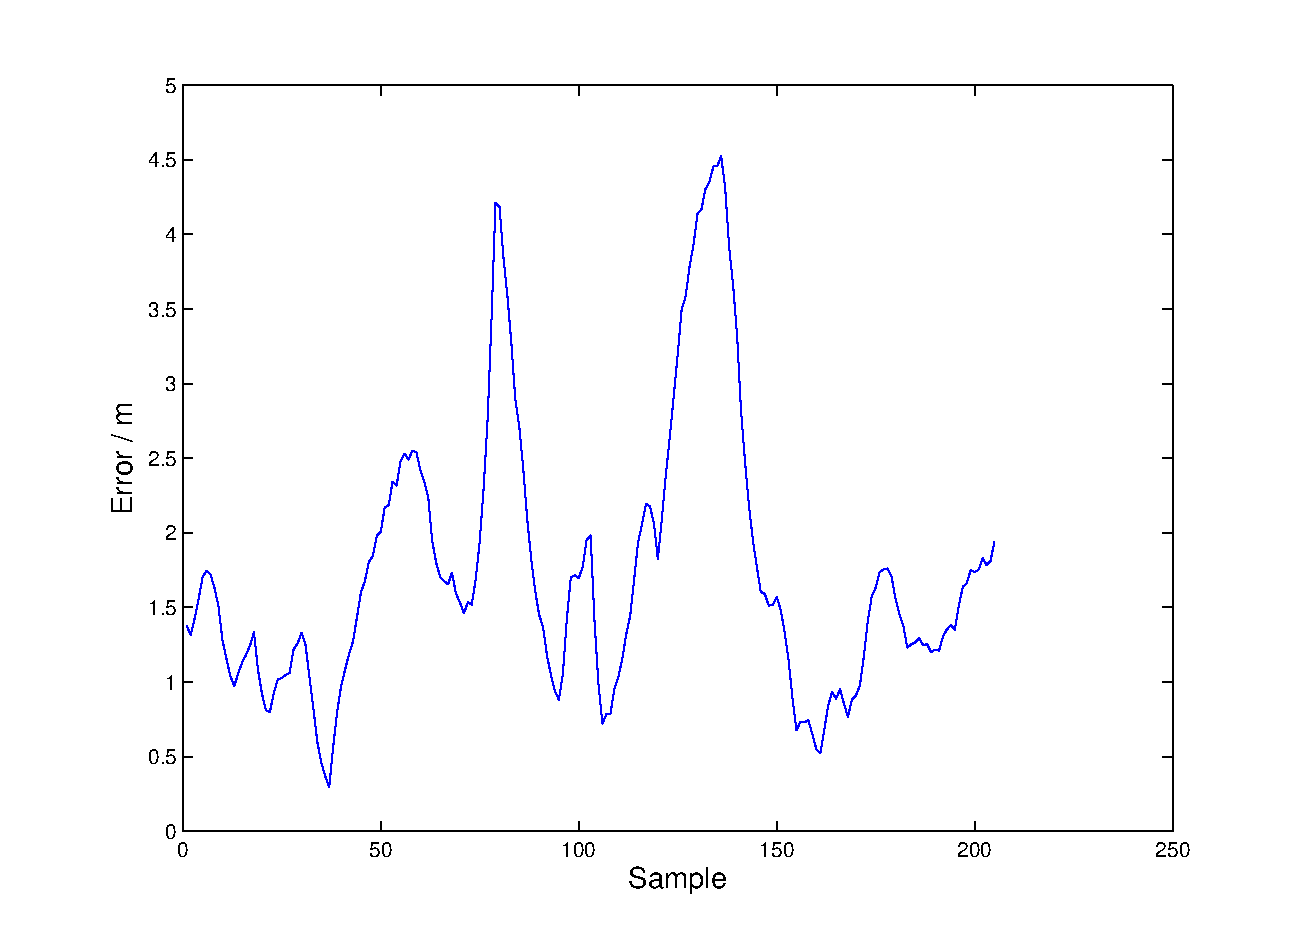
\includegraphics[width=1\textwidth ]{images/pure_rssi/error_env_1_05}
\caption{The absolute errors in estimated position for \emph{environment one}.}\label{error_env_1_05}
\end{figure}
%
The methodology from \emph{case 1} was used during this test and measurements from seven APs along a path of approximately one hundred meters. The locations of the APs together with the path taken may be found in Figure \ref{env_one}.

The estimated walked path using RSSI measurements is presented in Figure \ref{true_vs_est_env_1_05} and the absolute position errors in Figure \ref{error_env_1_05}. Some additional data concerning the error is presented in Table \ref{table:error_env-1}.
%
\begin{table}
\begin{center}
\begin{tabular}{|l|c|}
\hline
\multicolumn{1}{|c|}{Attribute} & Meter \\
\hline
\hline
Mean & $1.7$ \\
\hline
Maximum & $4.7$\\
\hline
Median & $1.5$ \\
\hline 
\end{tabular}
\end{center}
\caption{Attributes of the absolute positioning error for \emph{environment one}.}\label{table:error_env-1}
\end{table}

In this environment the placement of the access point in relation to the path walked is beneficial. During the walk, measurements from at least four APs are available and almost always on both $2.4$ and $5$ GHz.  Further, the geometry of the APs is such that we always stay inside or at the border of a polygon where the APs compose the corners. These properties contributes to the fairly small positioning errors in Table \ref{table:error_env-1}  
%
\subsection{Environment Two - WORKING TITLE}
%
The test in \emph{environment two} uses the methodology of \emph{case 1} and the measurements are taken over a distance of $176.5$ meters, for a reference of the actual path see Figure \ref{true_vs_est_env_2_05}.    
%
\begin{figure}[!hbt]
\include{graphics}
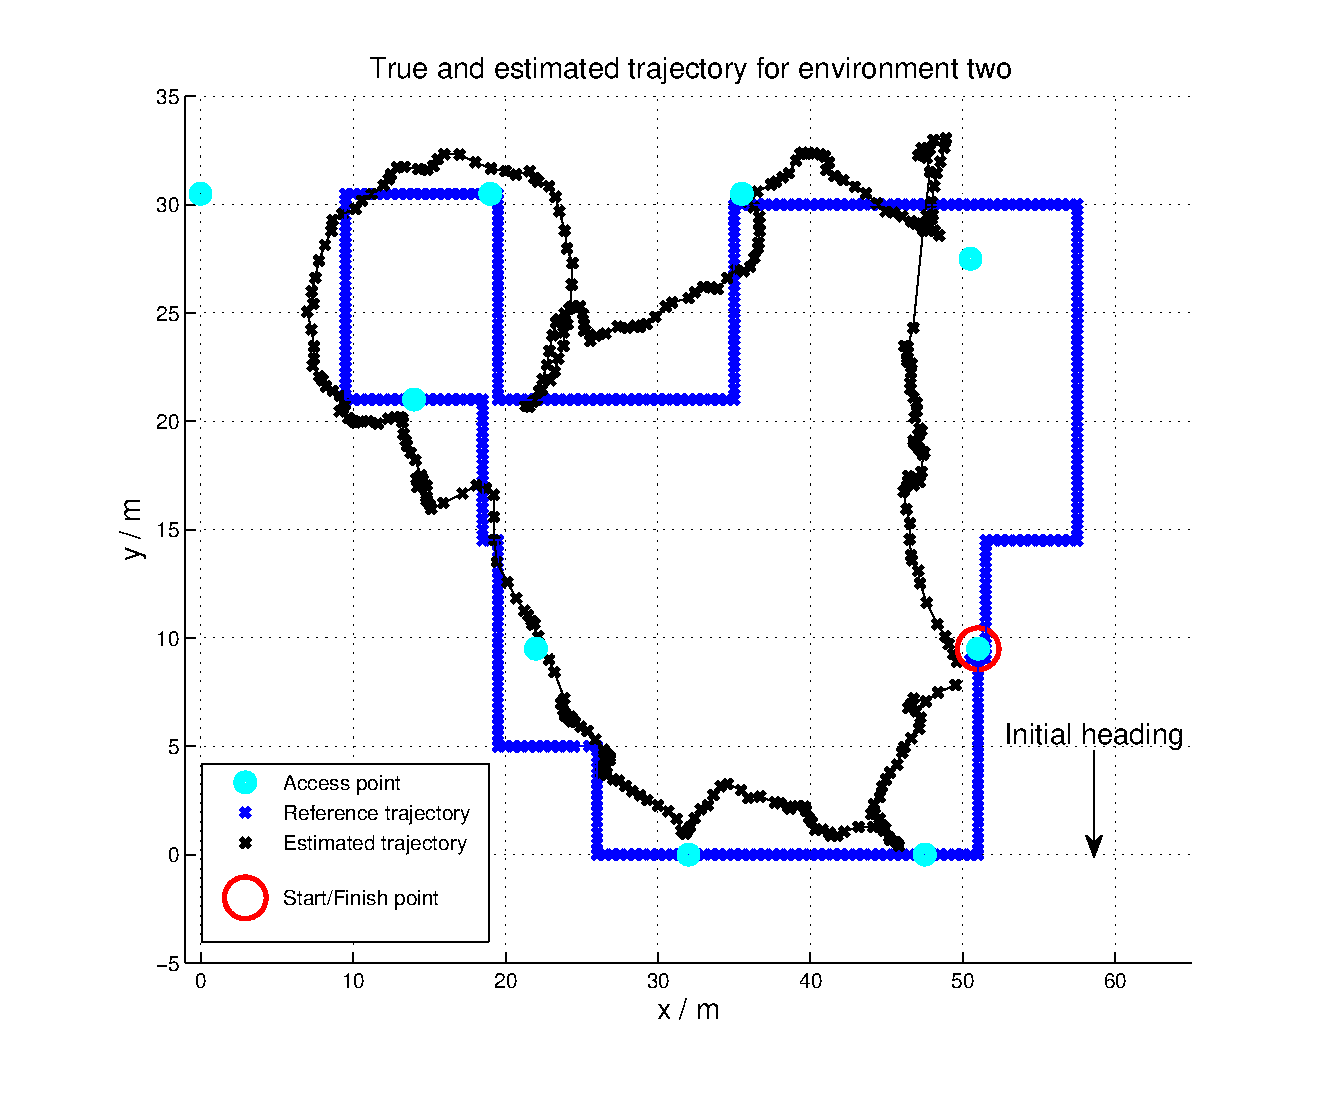
\includegraphics[width=1\textwidth ]{images/pure_rssi/true_vs_est_env_2_05}
\caption{The true path (\emph{blue}), along with estimated path (\emph{black}), start point (\emph{red} \texttt{o}), initial heading (\emph{black} arrow) and access point (\emph{cyan} \texttt{o}).}\label{true_vs_est_env_2_05}
\end{figure}
%
\begin{table}[!hbt]
\begin{center}
\begin{tabular}{|l|c|}
\hline
\multicolumn{1}{|c|}{Attribute} & Meter \\
\hline
\hline
Mean & $4.0$ \\
\hline
Maximum & $11.5$\\
\hline
Median & $3.2$ \\
\hline 
\end{tabular}
\end{center}
\caption{Attributes for the absolute positioning errors for \emph{environment two}.}\label{table:error_env_2}
\end{table}

A plot of the estimated path along with the true one is shown in Figure \ref{true_vs_est_env_2_05} and some attributes of the absolute positioning error can be found in Table \ref{table:error_env_2}.

The maximum positioning error here is considerably worse than the maximum from \emph{environment one}. This is largely due a unfavorable geometry of the APs during the last part of the path where only measurements from the three rightmost APs where available. Theses APs compose a quite obtuse triangle further impairing the positioning.  
%
\subsection{Environment Three - WORKING TITLE}
%
For environment three which was a substantially longer path of around 300 meters (273 m), the \emph{case 2} methodology was used. Measurements where received around once every 3rd second, resulting in the measurements being taken over a distance of around $4.5$ meters and a total of 61 different measurements points were collected. 

In Figure \ref{true_vs_est_env_3}, the true path along with estimated positions and path, may be viewed. For this test case, it is hard to give a absolute measurement of the error. Instead, one has to consider the difference between true and estimated path. Further, the measurements was taken while moving at constant speed and the time between each measurements is more or less constant. Thus, the estimated positions should be approximately equally spaced over the path. The estimated path differs from the true one at times, but the difference is, in absolute terms, not large. Also, most of the estimated positions are equally spaced. However, a few of them stands out and the minimum distance between two is $0.49$ m and maximum $8.2$ m. Another interesting observation is that the mean distance between two consecutive estimated positions is $4.1$ m giving a total distance of $250$ m, which is $23$ m less than the true path. This is also visible in Figure \ref{true_vs_est_env_3} in that the estimated path have a tendency to cut corners.         
%
\begin{figure}[!hbt]
\include{graphics}
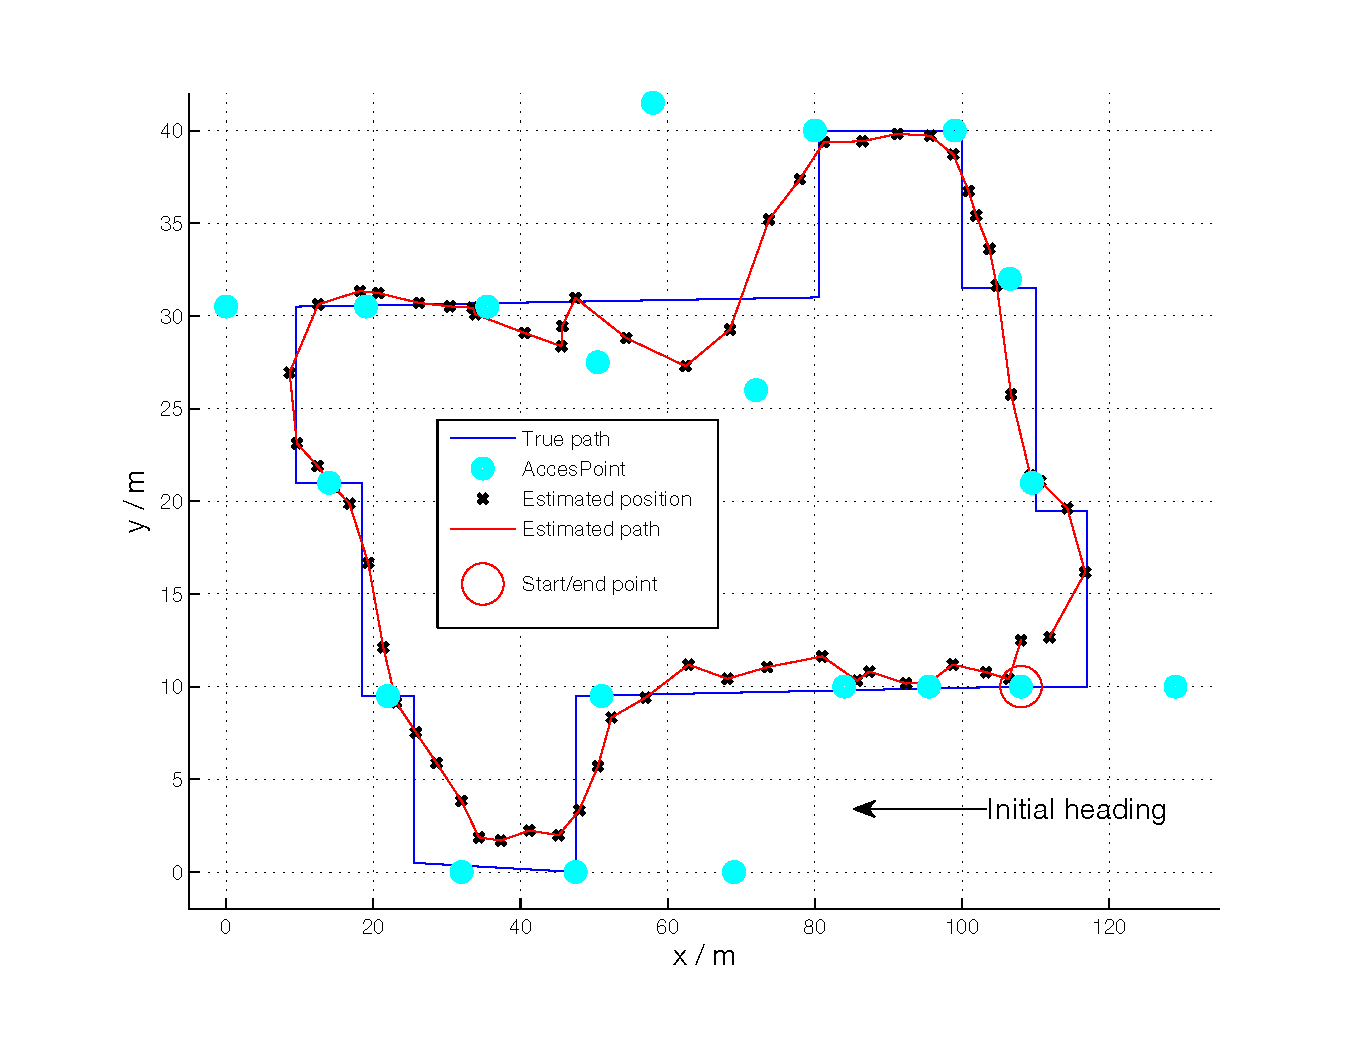
\includegraphics[width=1\textwidth ]{images/pure_rssi/true_vs_est_env_3}
\caption{The true path (\emph{blue}), along with estimated path (\emph{red}), estimated positions (\emph{black} \texttt{x}), start point (\emph{red} \texttt{o}), initial heading (\emph{black} arrow) and access point (\emph{cyan} \texttt{o}).}\label{true_vs_est_env_3}
\end{figure}
%
\subsection{Least Squares - a Comparison}
%
A common way of estimating a position from a RSSI measurements is to use a least squares (LS) estimation, for additional information see \ref{sec:oet}. Here the difference between the estimations from a particle filter (PF) and from a LS algorithm will be investigated. 

The comparison will be made for environment \emph{one} and \emph{two} from the previous sections, but with new datasets. Further, the methodology from \emph{case }1 will be used, but with 3 m instead of $0.5$ m sample spacing.This methodology is used to be able to measure the absolute position error from the different estimators. Further, both estimators will use the same path loss models.   
%
\begin{figure}[!hbt]
\include{graphics}
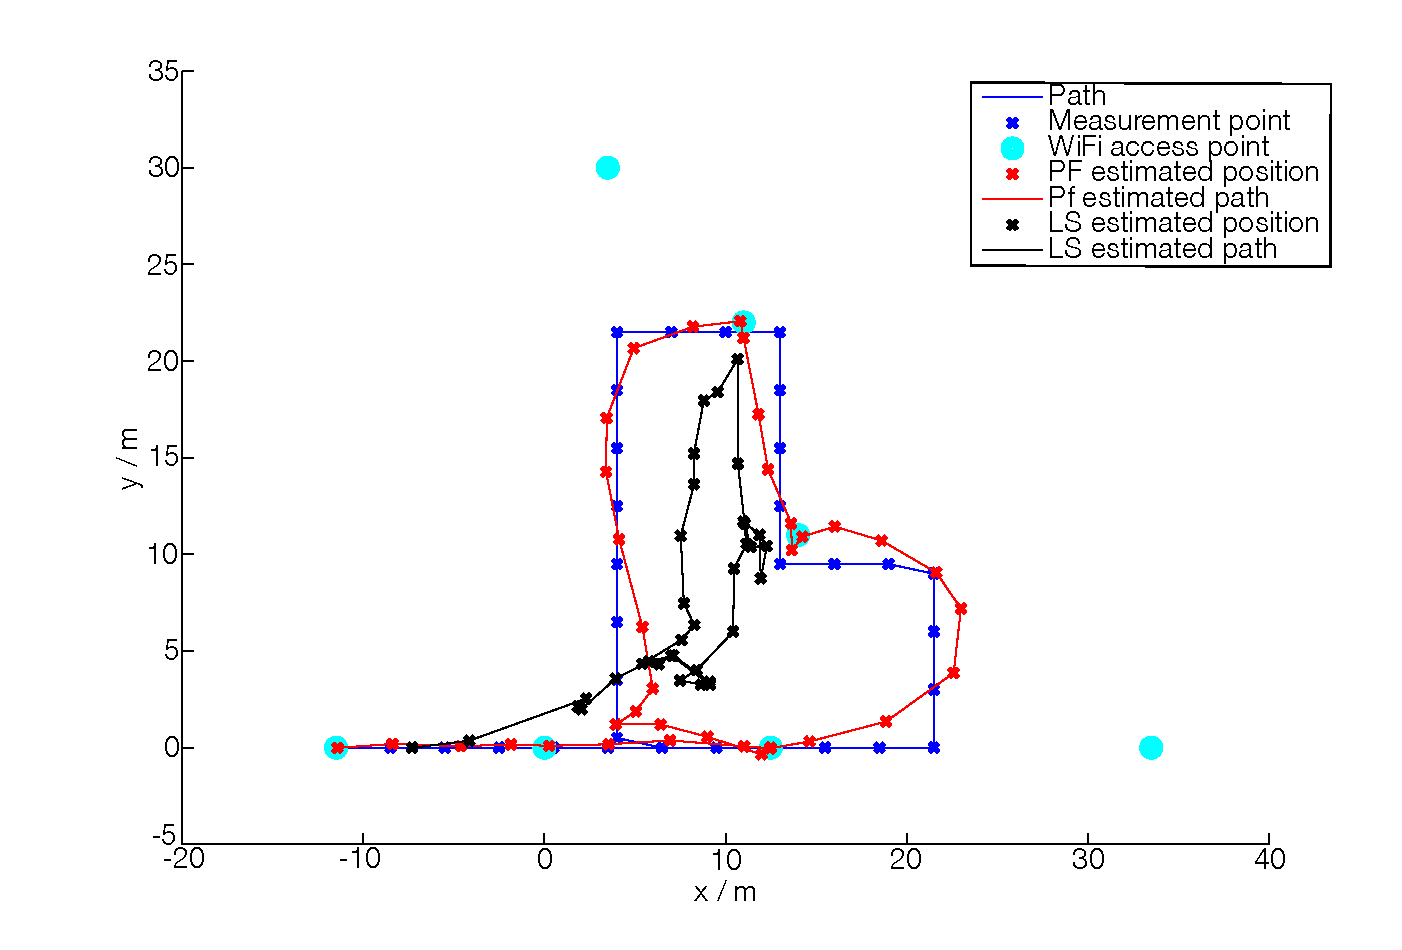
\includegraphics[width=1\textwidth ]{images/pure_rssi/ls_short_path}
\caption{Least squares estimation versus particle filter estimation for environment \emph{one}. True path (\emph{blue}), LS estimated path and position (\emph{black})and PF estimated path and position (\emph{red})}\label{ls_short}
\end{figure}
%
\begin{figure}[!hbt]
\include{graphics}
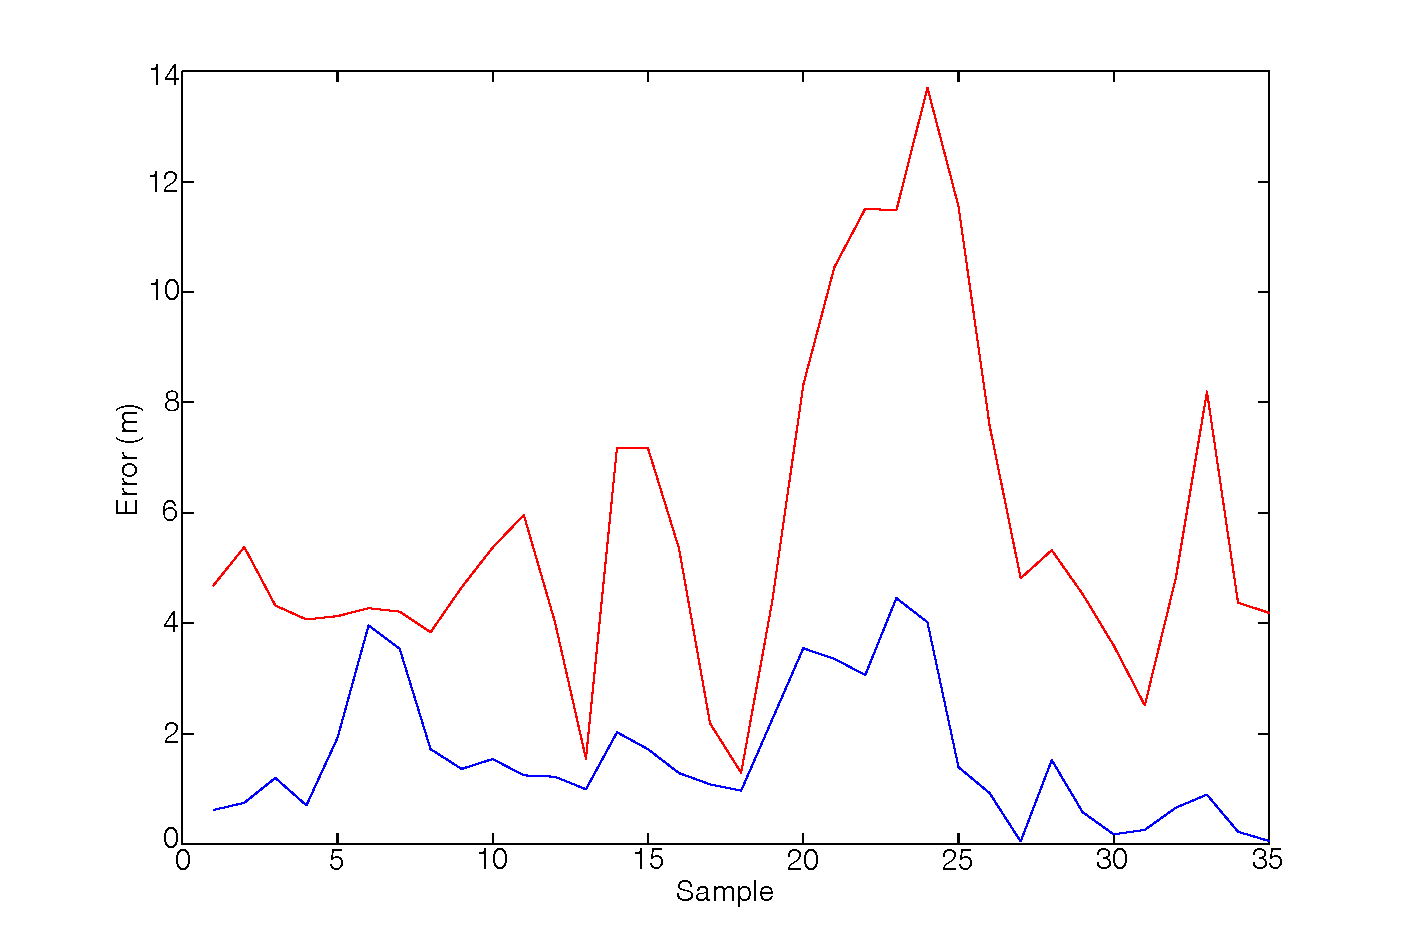
\includegraphics[width=1\textwidth ]{images/pure_rssi/ls_error_short}
\caption{Absolute position error for the LS (\emph{red}) and PF (\emph{blue}) estimators for environment \emph{one}.}\label{ls_error_short}
\end{figure}
%
\begin{figure}[!hbt]
\include{graphics}
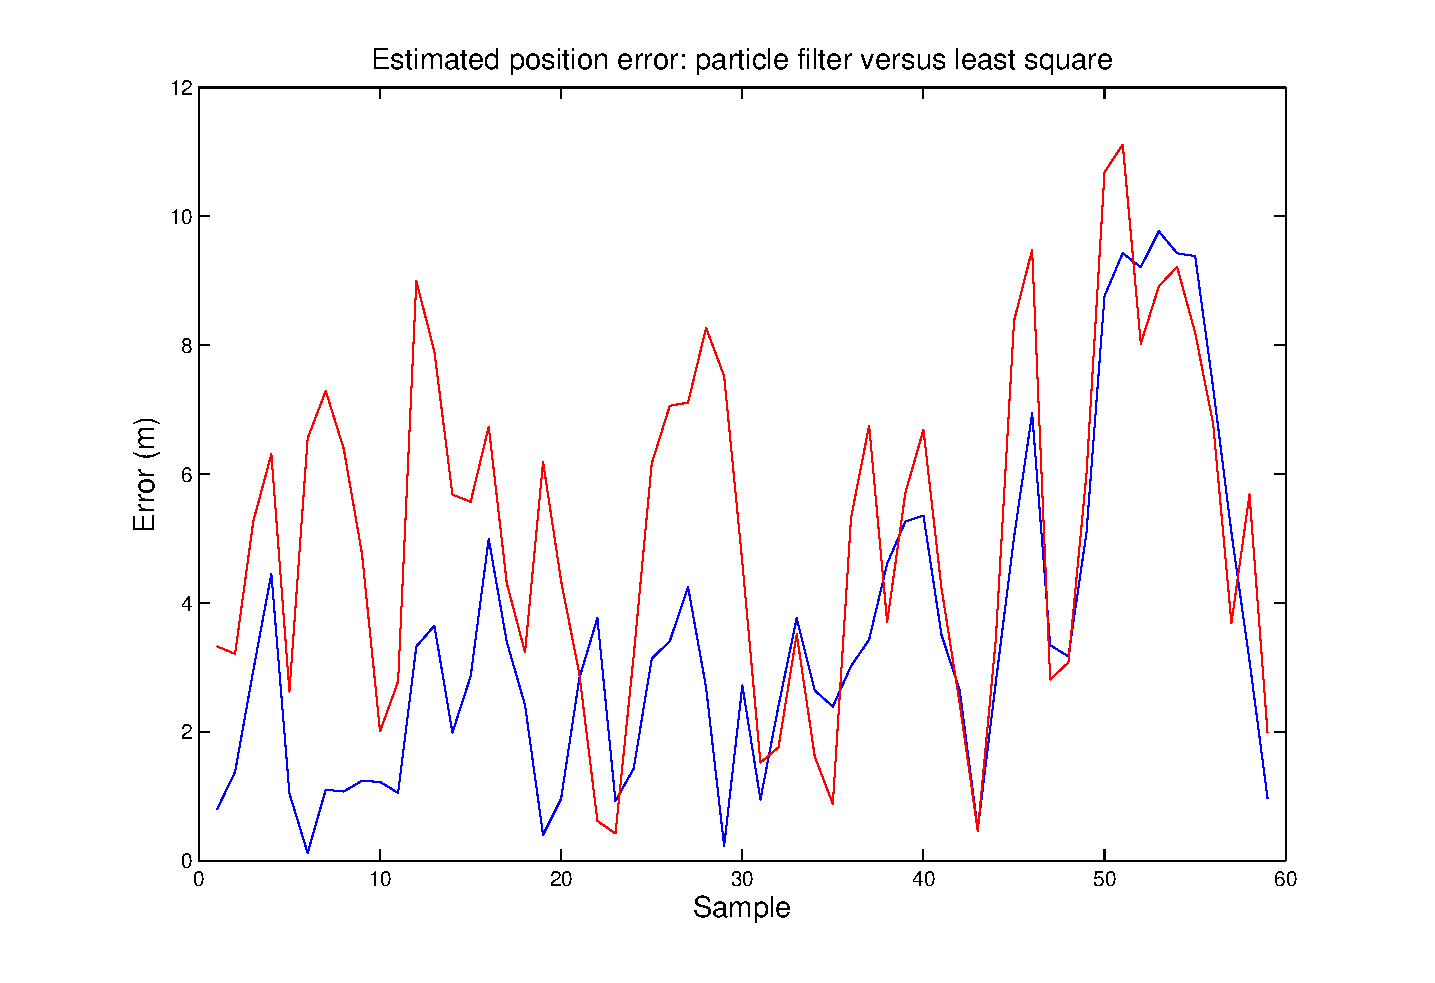
\includegraphics[width=1\textwidth ]{images/pure_rssi/ls_error_medium}
\caption{Absolute position error for the LS (\emph{red}) and PF (\emph{blue}) estimators for environment \emph{two}.}\label{ls_error_medium}
\end{figure}

The estimated path from both the PF and LS estimators is displayed in Figure \ref{ls_short} along with the true path for environment \emph{one}. It is clearly visible that the PF performs considerably better compared to the LS estimator. The positioning errors from Figure \ref{ls_error_short} makes this even more clear and the PF has a smaller positioning error for every sample compared to the LS estimator. The mean position error is, for the PF  $1.7$ m and for the LS estimation, $5.7$ m. 

For environment \emph{two} the LS estimation perform better in comparison to the PF, as shown by the errors in Figure \ref{ls_error_medium}. The PF, however, does still provide the best position estimates and the error is lower for the PF in most of the samples and the LS estimator produces the larges position error. The difference in maximum error though is not large, then again, the mean error for the PF is $3.4$ m and for the LS estimation, $5.1$ m. The PF seams to produce considerably better results compared to the LS method when the environment is favorable i.e when a large number of access point are available and/or their geometry are good. When the conditions are disadvantageous both methods performs equally, giving positions around 10 meters off.

The conclusion to be drawn from these investigations is a particle filter is the better choice for estimating positions from noisy RSSI measurements, especially if the only sought after attribute is the smallest mean and maximum errors. The lest squares estimation may be desirable to use if simple implementation is important or if limited computing power is available.

An interesting aspect is the performance when no previous measurements are available. Then, the PF loses its advantage of using these, whereas nothing changes for the LS. A new test was performed in \emph{Environment two}, and at each measure point, the previous position was treated as completely unknown. This means that the particles had to be spread out over the whole floor before each estimation. Then, one iteration was performed in the PF. The errors are shown in Figure XXXXXX. The mean error is 5.09 m for the PF and 5.14 m for the LS. It is difficult to decide which method that works best in this case. 

%
\section{Concluding remarks}
%
Using measurements of RSSI to position devices in a indoor environment can be a satisfactory technique if the need for precision is not too great. In a fairly homogenous building, i.e approximately the same path loss model within, with a reasonable number of access point placed in a acceptable geometry, the positioning may be quite good. 

The position estimation may, with satisfactory result, be computed using a particle filter. The PF outperforms a least squares estimation in most cases and newer produces inferior results for a sustained timespan. The worse case error between the two estimators is on par when the environment is unfavorable but the PF produces better estimates in a beneficial environment and smaller mean errors in the long run. 

A few objections with the technique must however be mentioned, first and foremost, more or less all buildings needs a specific path loss model and the power which each AP transmits, and their location, needs to be known. Also, to have a chance to obtain a reasonable position estimate measurements from at least three different APs must be available at all times. If fewer are available larger positioning errors are to be expected, if only two AP are visible at least two positions will be equally probable and if only measurements from one is available all point at a certain distance may be the true position. The position history of the PF can improve the estimation when the geometry is unfavorable if the initial position is fairly accurate and the time spent in the environment is rather short. The LS estimation lacks this property and will produce erroneous or inconsistent estimations independent of past positions. Further, antennas have different abilities to receive signals, thus the behavior of the specific device must be known. Lastly, how different users hold or carry their devices substantially affect the received signal power.  

On the other hand, most newly constructed or renovated building already have plenty of APs and there this technique may provide a simple and cost effective way of providing indoor positioning. If methods for finding APs and estimating the path loss model in a simple way can be attained the setup may even be quite simple. If some of the user induced signal blockages can be registered and compensated for as well, the technique might be useful for tracking people even when they do not carry their device in hand. This only leaves the problem of characterizing the behavior of the antenna for each device, but as this only needs to be done one time for each type of device, it is no overwhelming task.        
%
\chapter{Adapting the Model Parameters} %Working title
%

In the previous chapter, the parameters $\alpha$ and $C$ in the path-loss model 
%
\begin{equation}
\log_{10}({P_r(d)})=C-10n\log_{10}(d) - \alpha\cdot\min({d, d_{\text{max}})}+ X_\sigma.
\label{equation:model_to_adapt}
\end{equation}
%
were assumed to be known. However, these constraints are not necessary if the parameters can be estimated during the localization. This is useful since $\alpha$ depends on the current environment, and $C$ depends on the radiated power from each AP. The first part of this chapter describes an algorithm for determining when the estimation of the location is accurate, and using this to estimate the model parameters. 

Another issue is that the signals reaching the phone might be attenuated considerably by the user. The weaker signals would indicate that the phone is further away from each AP than it actually is. In the second part of this chapter, an algorithm to compensate for this is proposed and evaluated.

%
\section{Estimation of Position Error} %Working title
%
\begin{figure}[!hbt]
\include{graphics}
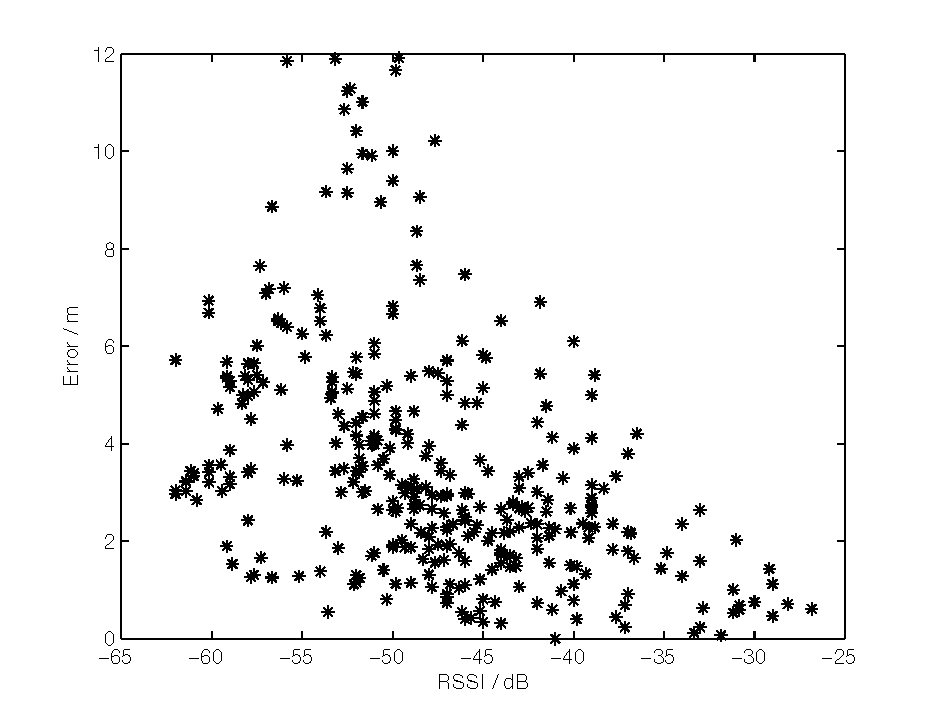
\includegraphics[width=1\textwidth ]{images/adapt_parameters/error_vs_maxP_all}
\caption{Figure text}\label{error_vs_maxp_all}
\end{figure}
%
\begin{figure}[!hbt]
\include{graphics}
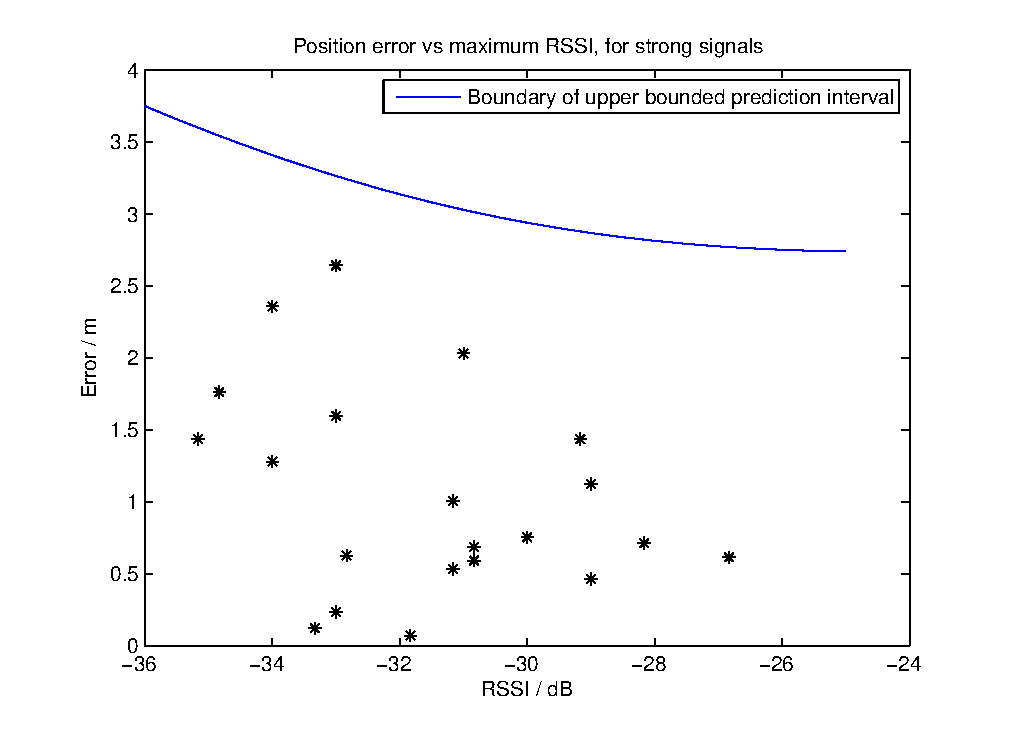
\includegraphics[width=1\textwidth ]{images/adapt_parameters/prediction_interval}
\caption{Figure text}\label{prediction_interval}
\end{figure}

The method described in Chapter \ref{chap:pure_rssi} has proven to perform better at a closer distance to the nearest AP. At a certain time step, a large maximum RSSI-value indicates that the nearest AP is close. This, in turn, indicates that the position error is relatively small. Figure \ref{error_vs_maxp_all} shows this relation. The data is from the test setup \emph{Case 1} for \emph{Environment Two}, defined in Section \ref{sec:test_setup} and \ref{environment_results}, respectively.

Whenever one RSSI is above a certain value, the error can be considered small. This value depends on the model of the phone, and on $C$ for the closest AP. In this example, -36 dB is a suitable lower limit. If one RSSI is larger than that at a certain time, the average error is 1.05 meters, and it is unlikely to get an error that is larger than 4 meters. Figure \ref{prediction_interval} shows the error together with a one-sided, upper bounded, 99\% prediction interval \cite{matstat}. For other phone models and different AP:s , the limit has to be modified by adding a constant value, in order to get similar results. If $C$ is not known initially, it has to be estimated in order to determine the limit, before the adaptation can begin.  This can be solved when the user walks straight below an AP for the first time. By registering the peak RSSI, a very first approximation of $C$ can be computed, and a reasonable limit determined.

%
\section{Updating the Parameters} %Working title
%
In order to successfully determine $\alpha$ and $C$, an accurate estimation of the position is required. The previous section described how a maximum RSSI larger than a certain limit indicated a low position error. Therefore, the algorithm performs a calibration when this limit is exceeded. Expressions for each parameter can be determined by \ref{equation:model_to_adapt}, which yields

%
\begin{equation}
\alpha=\frac{C-10n\log_{10}(d)-\log_{10}(P_r)}{\min({d, d_{\text{max}})}}
\label{equation:update_alpha}
\end{equation}
%

%
\begin{equation}
C = \log_{10}(P_r)+10n\log_{10}(d)+\alpha\cdot\min({d, d_{\text{max}})}
\label{equation:update_c}
\end{equation}
%
The noise $X_\sigma$ is unknown and omitted in the parameter update. 
%
Since $\alpha$ and $C$ depend on each other, they should not be updated at the same time. Instead, $C$ is updated for the nearest AP only, whereas $\alpha$ is updated using the RSSI from the others. When $C$ is determined, the phone is assumed to be straight below the nearest AP, so that the distance $d$ consists only of the vertical distance $d_{\text{ver}}$. In this case, $d_{\text{ver}}$ = 2 meters. Moreover, this AP is assumed to be within LOS, i.e. $\alpha$=0. Hence, \ref{equation:update_c} can be rewritten as
%
\begin{equation}
C = \log_{10}(P_r)+10n\log_{10}(d_{\text{ver}})
\label{equation:update_c_simple}
\end{equation}
%
Furthermore, initial estimations of the constants are required. These have to be accurate enough for the algorithm to perform a first successful parameter update. Hence, the position estimation has to be accurate enough when an update is performed. 
%
The value of $C$ is specific for each frequency on each AP. Therefore, the algorithm should store one value of $C$ for each frequency on each AP.
The parameter $\alpha$ can be treated in different ways. Here follows two alternatives for this.

\subsection{Alternative 1}
Alpha is the same for the whole building. After each determination of $\alpha_i$, $\alpha_{ave}$ is defined as the average of all determinations, including the initial estimation.


%
\subsection{Alternative 2}
In this algorithm, each value of $\alpha_{ij}$ is stored in a matrix $\vec{\alpha}$. Here, $\alpha_{ij}$ is the parameter to be used in section $i$, for AP $j$. Each floor is divided into sections as follows:

Each AP corresponds to one circular section, centered at the AP and with radius $r_s$. These sections may overlap, and there might be areas that do not belong to any sector (see Figure \ref{alpha_sections}). Hence, the following three cases may occur for each particle:

\begin{figure}[!hbt]
\include{graphics}
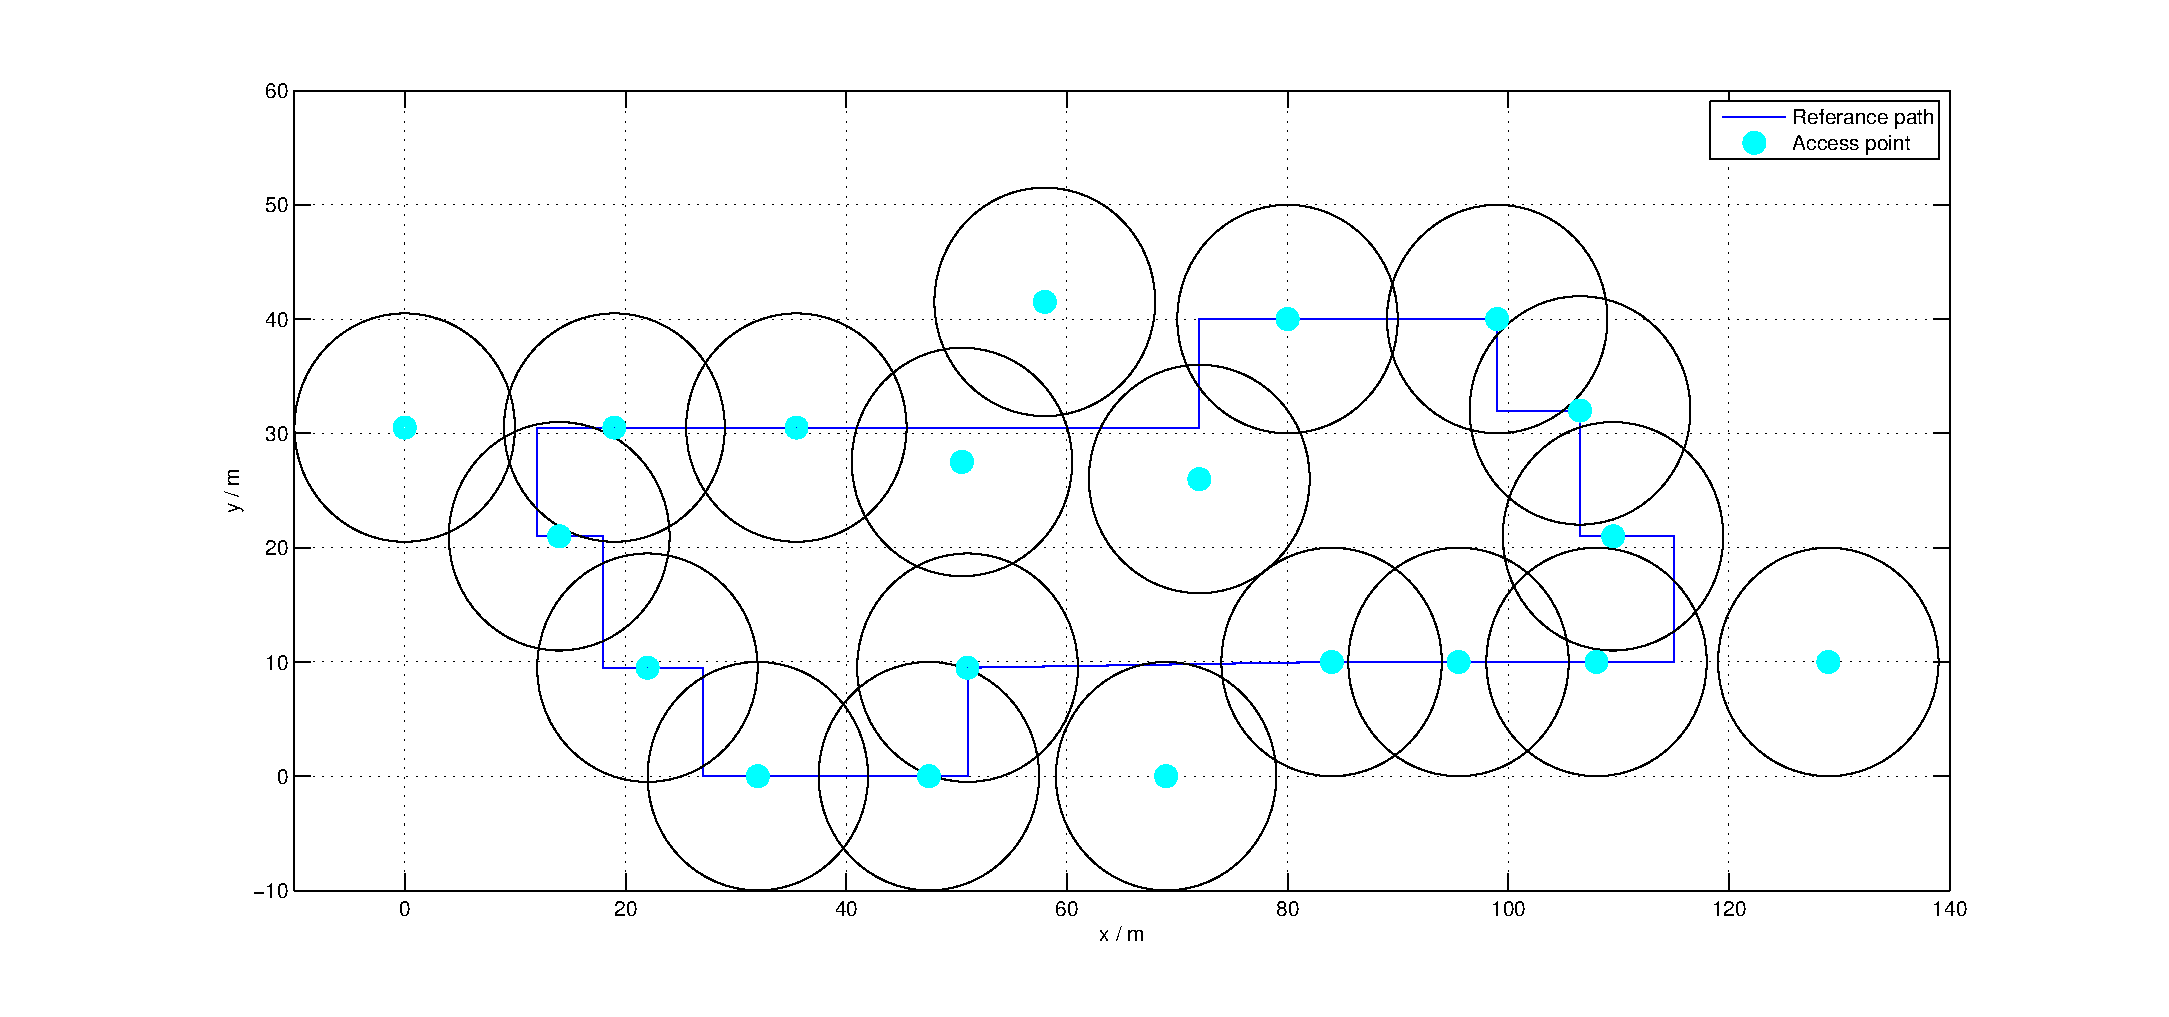
\includegraphics[width=1\textwidth ]{images/adapt_parameters/alpha_sections}
\caption{\emph{Environment three} divided into sections. Each circle corresponds to a section around a certain access point.}\label{alpha_sections}
\end{figure}


\subsubsection{1. Exactly one section}
If a certain particle is in section $k$ only, 
the parameter set from row $k$ in alpha will be used for this particle. 

\subsubsection{2. Several sections}
If it is in several sections at the same time, an average of the parameter sets for these sections will be used.

\subsubsection{3. No section}
Finally, if it is outside all sections, a default value of $\alpha$ will be used.

Please note that each particle gets its own set of parameters, and that the estimated position of the phone is not involved in choosing this set.
%
\begin{figure}[!hbt]
\include{graphics}
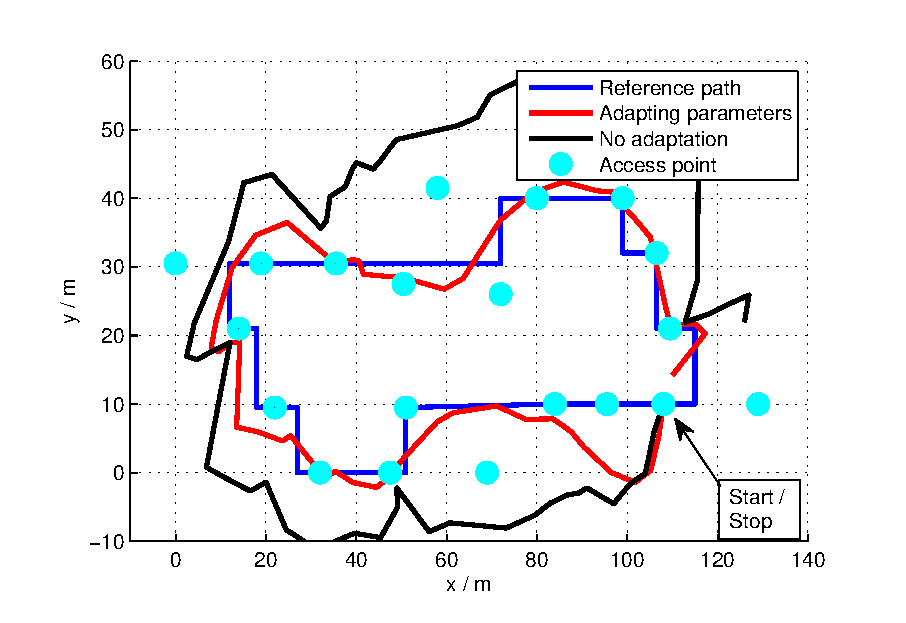
\includegraphics[width=1\textwidth ]{images/adapt_parameters/adaptation_vs_none}
\caption{}
\label{adaptation_vs_none}
\end{figure}
%
Both alternatives have been tested offline using $Malab$. For the environments defined in \ref{environment_results}, the results are similar. The reason why there is no gain in dividing the building into areas is that it is homogeneous enough for alternative 1 to work. In an environment where the obstacle density changes more, alternative 2 would be more suitable.

In order to evaluate the parameter updates, the algorithm was given erroneous initial parameter values. Then, the phone was carried one round in \emph{Environment three}, and after that the updated parameters were noted. During the round 61 RSSI measurements were taken by the phone, giving a approximate spatial separation of 4.5 meters. The resulting parameters are shown in Table \ref{table:parameter_adaptation}

\begin{table}[!hbt]
\begin{center}
\begin{tabular}{|c|c|c|c|c|c|}
\hline
\multicolumn{2}{|c|}{Initial values}
&\multicolumn{4}{|c|}{Values after adaptation} \\
\hline
\hline
\multicolumn{2}{|c|}{2.4 and 5 GHz}
&\multicolumn{2}{|c|}{2.4 GHz}
&\multicolumn{2}{|c|}{5 GHz} \\

\hline
$C$ & $\alpha$ & $C$ & $\alpha$& $C$& $\alpha$\\
\hline
-50 & 1.0 & -37.7 & 0.28 & -35.8 & 0.35\\
\hline
-45 & 0.9 & -37.7 & 0.25 & -35.8 & 0.34\\
\hline
-35 & 0.5 & -35.6 & 0.35 & -33.7 & 0.42\\
\hline
-25 & 0.3 & -31.5 & 0.47 & -29.6 & 0.54\\
\hline
\end{tabular}
\end{center}
\caption{Parameter values before and after adaptation.}\label{table:parameter_adaptation}
\end{table}

Implausible parameter values (e.g. $C = -50$ or $C = -25$) are more reasonable after the adaptation. Moreover, the algorithm moves the parameter values towards the region with relatively low position error in Figure \ref{err_vs_param}. The bottom row in \ref{table:parameter_adaptation} was investigated in more detail, as an example of how the adaptation affects the positioning. Figure \ref{adaptation_vs_none} shows the positioning with and without the parameter adaptation, respectively, with $C = -25$ and $\alpha = 0.3$ as initial values.

\section{Compensating for Signal Block} %Working title
%

The RSSI is affected by how the phone is carried by the user. If, for example, the user blocks the signals with the hand, RSSI will get lower, which indicates that the phone is further away from each AP than it actually is. In this section, this effect, and the possibility of compensating for it, will be evaluated.

\subsection{Evaluation of different use cases}
In the tests this far, the phone has been held so that the signal is blocked as little as possible. In this section, three different use cases are tested, all in \emph{Environment three}. 

\subsubsection{1. Phone in pocket}
In this test, the phone was first carried one round in the hand. After that, it was moved to the jeans side pocket, and then another round was walked.

\subsubsection{2. Blocking with hands, once}
Again, the phone was carried one round in the hand. Then, the user tried to block as much of the signals with the hands as possible during the second round the hands.

\subsubsection{3. Blocking with hands, repeatedly}
Like the previous test, but during the second round, the signals were blocked and unblocked repeatedly. 

The results are shown in Figure \ref{positioning_pocket} , \ref{hand_block} and \ref{hand_block_repeatedly}.



\begin{figure}[!hbt]
\include{graphics}
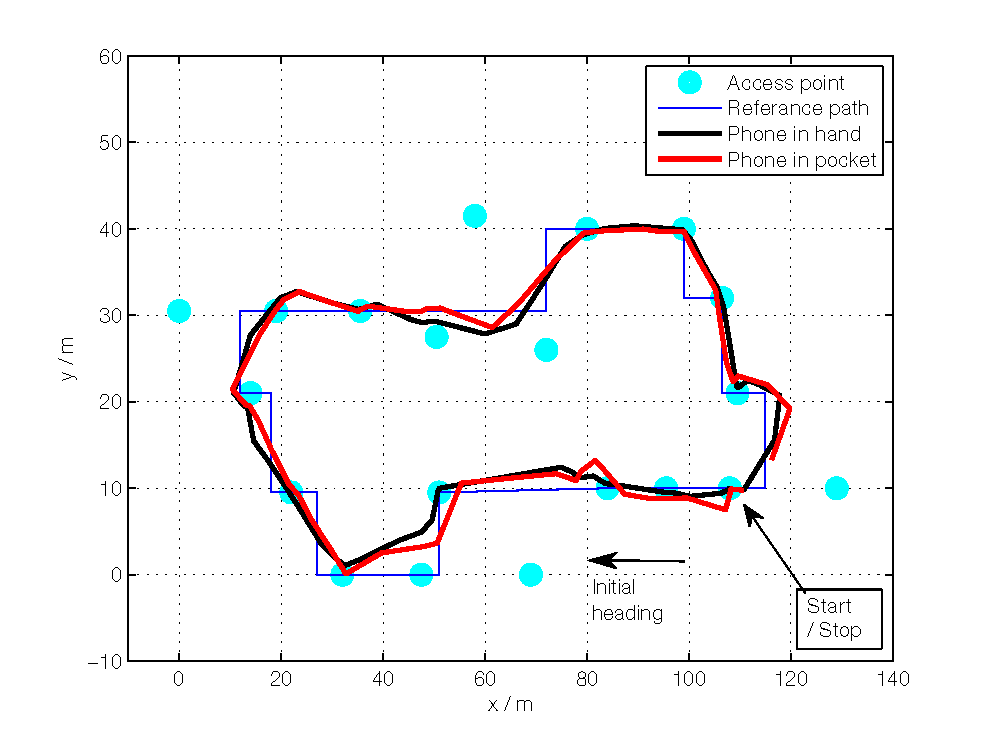
\includegraphics[width=1\textwidth ]{images/adapt_parameters/positioning_pocket}
\caption{Phone in pocket. Wearing the phone in the pocket did not affect the positioning significantly}\label{positioning_pocket}
\end{figure}

\begin{figure}[!hbt]
\include{graphics}
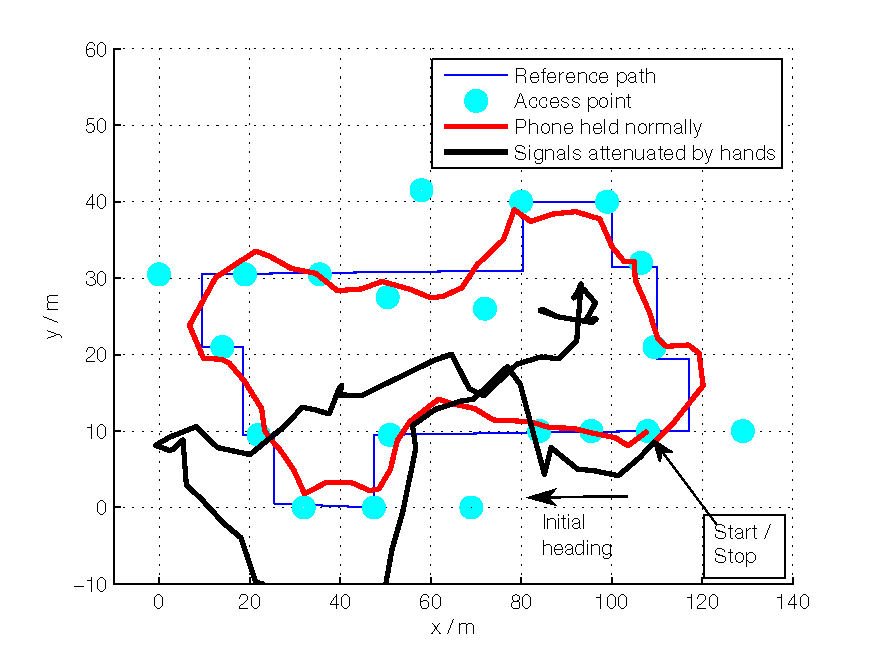
\includegraphics[width=1\textwidth ]{images/adapt_parameters/hand_block}
\caption{Blocking with hands, once. Attenuation by the hands had a severe impact on the positioning.}\label{hand_block}
\end{figure}

\begin{figure}[!hbt]
\include{graphics}
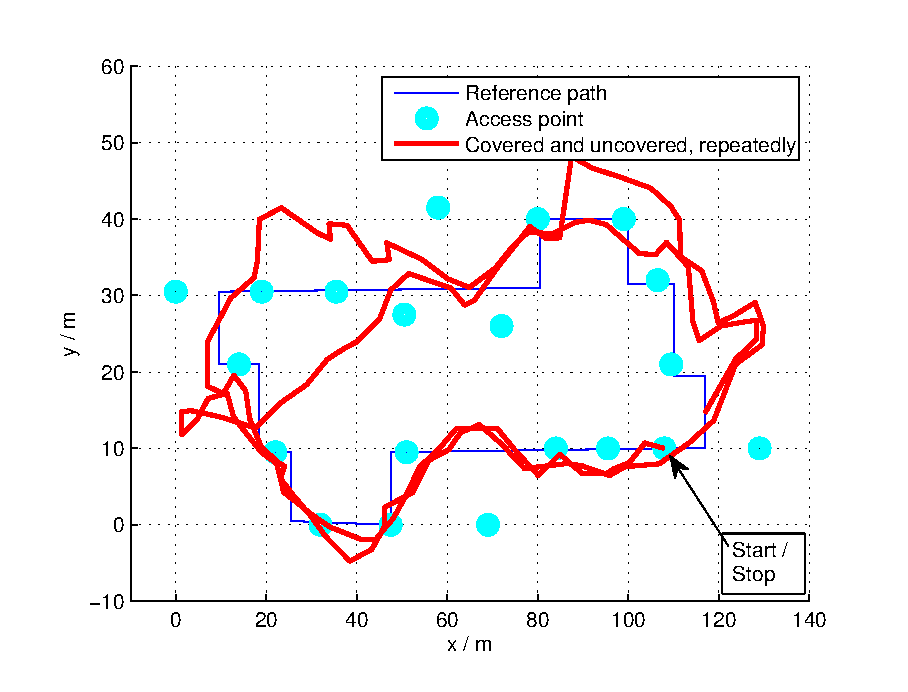
\includegraphics[width=1\textwidth ]{images/adapt_parameters/hand_block_repeatedly}
\caption{Blocking with hands, repeatedly. Attenuation by the hands had a severe impact on the positioning.}\label{hand_block_repeatedly}
\end{figure}
%
Carrying the phone in the pocket did not affect the RSSI significantly, and hence the positioning was unaffected. However, blocking the signals with the hands lowered the RSSI considerably, causing the positioning to be inaccurate. Hence, this use case has to be detected and compensated for.

\subsection{Compensation}

The main strategy for detecting the attenuation is to note when the RSSI decreases fast. However, moving away from the AP:s, or walking behind a wall, may lower the RSSI in a similar way. In order to distinguish the signal attenuation by the user only, the algorithm focuses on the six largest RSSI-values. If the average of these decrease more than 6 dB in one time step, this indicates hand attenuation. Moving away from the AP:s would not make the RSSI decrease that fast, and if LOS is lost to some AP:s there is a chance that LOS is established to another. If on the other hand LOS is lost to several AP without gaining LOS to other AP, e.g. entering a room without an AP, the compensation may be triggered. However, this is more likely to improve than to degrade the positioning as the standard RSSI models do not incorporate quick drops in signal level caused by walls and similar objects. If a user enters a room without an AP, the RSSI measurements would drop significantly to all AP:s, but the compensation would ideally remove this effect, allowing the walls to be taken into account by the positioning algorithm. 

When an attenuation is detected, a constant term $H$ is added to the model, which corresponds to how much the signals have been reduced. Hence, the new model is given by \ref{equation:hand_comp}  When the phone is unblocked, this is detected in an analogous way, and then $H$ is set to 0. 

\begin{equation}
\log_{10}({P_r(d)})=C-10n\log_{10}(d) - \alpha\cdot\min({d, d_{\text{max}})}+H+ X_\sigma.
\label{equation:hand_comp}
\end{equation}

Test 1) and 2) were performed again, but this time with the compensating algorithm. The results are shown in Figure \ref{hand_block_comp} and \ref{hand_block_repeatedly_comp}.

\begin{figure}[!htb]
\include{graphics}
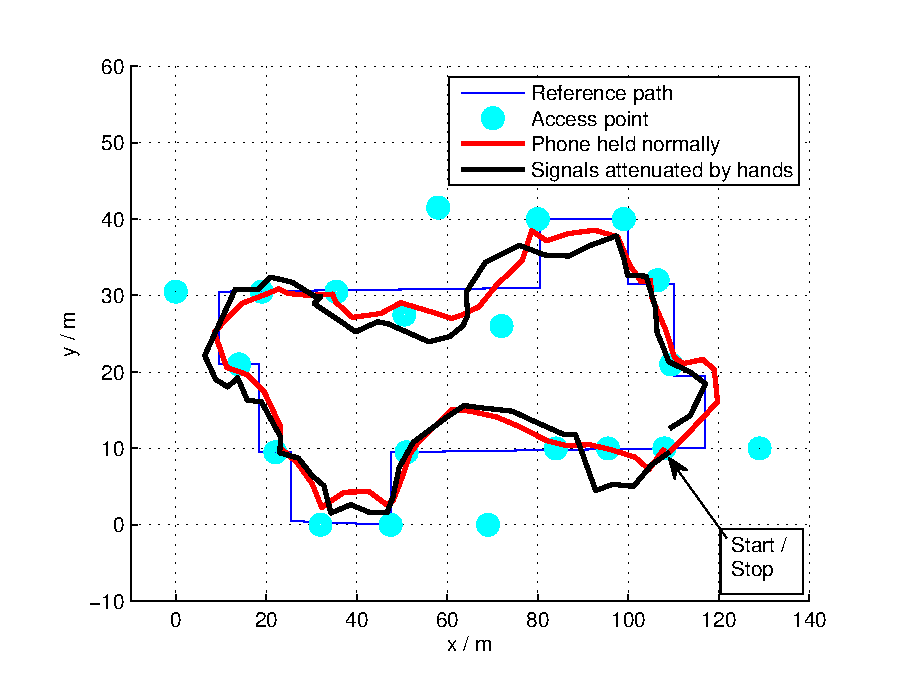
\includegraphics[width=1\textwidth ]{images/adapt_parameters/hand_block_comp}
\caption{Blocking with hands, once. The algorithm compensates for the attenuation.}\label{hand_block_comp}
\end{figure}

\begin{figure}[!htb]
\include{graphics}
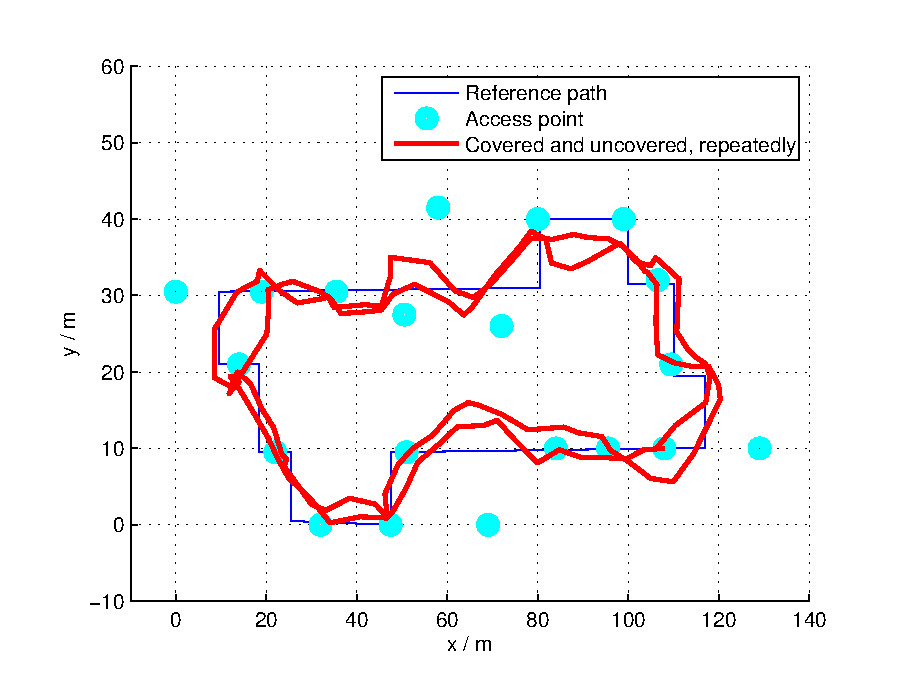
\includegraphics[width=1\textwidth ]{images/adapt_parameters/hand_block_repeatedly_comp}
\caption{Blocking with hands, repeatedly. The algorithm compensates for the attenuation.}\label{hand_block_repeatedly_comp}
\end{figure}


\section{Conclusion}
In this chapter, an algorithm that updates the model parallel to the positioning has been suggested. The purpose is to increase the generality of the application, and making it improve while in a new environment.


Compensating for the hand attenuation clearly improved the positioning. However, $H$ can not be determined exactly, due to noise and obstacles in the environment. In addition, the hand attenuation is only detected if the phone is covered fast enough. If it goes from uncovered to covered successively, during several time steps, this can not be distinguished from other causes of lowered RSSI. Naturally, going from covered to uncovered works analogously.

\chapter{Modeling the Kinematics} %Working title
%
Modeling the kinematics may greatly improve the performance of a positioning system, especially if the estimated position is noisy or biased. The kinematics may also be used to estimate the position in between the updates from the main positioning algorithm. The range of models stretches from simple random walk processes to estimating acceleration, velocity and position in a three dimensional space using sensor fusion.

After a short description of different random walk processes, quaternions are introduced and their use in three-dimensional pose  estimation, without risk of singularities, explained. A section about positioning using only sensors, named \emph{dead reckoning}, is presented, after which the chapter closes by a discussion of kinematics models used in indoor positioning and their effects on the performance.   
%
\section{Sensors}
Here follows a brief description of three sensors commonly available in modern smartphones, \emph{the accelerometer, the gyroscope} and \emph{the magnetometer}. A short description of their inner workings, advantages and disadvantages is given along with a description of their use in position estimation. For a deeper description of the sensors and a more extensive discussion about biases and drifts a reference is given to \cite{bently88} and \cite{morris96}. 
%
\subsection{The Accelerometer}
%
A accelerometer is a sensor measuring acceleration (m/s$^2$) along a certain axis. This is done by the accelerometer measuring the acceleration associated with the phenomenon of weight associated with a test mass at rest in the accelerometers frame of reference. To exemplify, an accelerometer at rest on the earths surface measures a acceleration, g = $9.81$m/s$^2$. Further, an accelerometer in free fall in space will measure no acceleration. Today most accelerometers measures acceleration along three orthogonal axis, thus giving information about the three dimensional acceleration. 

The fact that every object at rest at earth experience the acceleration associated with gravity poses a problem when using the accelerometer since the gravity always will be present in the measurements. This needs to be managed in some fashion. The simples is to keep the accelerometer fixed in reference to the earths coordinate system introducing gravity as a constant bias along a certain direction, which is easy to subtract. A more challenging case is when the accelerometer changes its orientation compared to the earths coordinate system. Here an algorithm to keep track of the accelerometers orientation is needed if the effect of gravity is going to be deductible. 

Another interesting aspect of gravity in relation to the accelerometer is the ability of finding out the accelerometers orientation in reference to the earths coordinate system. This is possible if the accelerometer does not experience any significant acceleration except for gravity. Then the accelerometers orientation may be determined by the component of gravity present on each of its axis. 

In principle the accelerometer could be used to estimate a position by integrating its output two times in respect to time. In practice, however, this is hard as the gravity needs to be accurately subtracted from the measurements if not to introduce a large positioning error. If even 1 \% of gravity is left in the measurements it will introduce a error of around 500 meters over 100 seconds. Further, the accelerometers present in todays smartphones suffers from biases and drifts which needs to be accurately evaluated if not to further degrade the position estimate. 
%
\subsection{The Gyroscope}
%
A gyroscope measures the \emph{angular velocities} with which it is turning around each its axis. Most gyroscopes uses three orthogonal axis giving measurements of the angular velocities on the form $\vec\omega = (\omega_x \hspace{5pt} \omega_y \hspace{5pt} \omega_z)$.  Mechanically, a gyroscope consist of a spinning wheel or disc mounted in a gimbal, a pivoted support that allows the disc to rotate freely about all three axis. This construction allows the disc to keep a almost fixed position in reference to the mounting platforms motion. However, this is a fairly large device not well suited for modern electronic devices. These instead rely on \emph{MEMS gyroscopes} which can be fashioned into a more suitable size. MEMS or \emph{vibrating structure} gyroscopes relies on the physical principle of vibrating objects tending to continue vibrating in the same plan as its supports rotate.  

As the MEMS gyroscope measures angular velocities and, in this thesis, the angular change is of interest, a method of computing them are needed. This is fairly simple, given two sets of angular velocities measured with a time difference of $\Delta t$, the angular change, $\theta$, may be computed using  numerically integration according to the \emph{trapezoidal rule} \cite{analysis},  
\begin{equation}
\theta=\Delta t \frac{\vec \omega _t +\vec \omega _{t+\Delta t}}{2}.
\end{equation} 
%
This can, of course, be applied to each of the gyroscopes axis, resulting in an estimation of how the gyroscope is turning and in extension, its orientation, in three dimensions. 

There are a few problems of using the gyroscope to determine the direction of movement. As it only measures how the angles change over time, the direction at the start of the navigation must be known and the orientation needs to be kept fixed in reference to the movement. For example, it is impossible do discern between a 90 degree turn and a mere turn of the gyroscope.  Furthermore, the gyroscope suffers from drifts and biases resulting in a growing heading error. Hence, if it is to be used for long stretches of time, the heading needs to be calibrated or only the difference between two fairly close (in time) angular estimation used. 
%
\subsection{The Magnetometer}
%
A way around the problems of a known initial direction is the use of a magnetometer, which measures the \emph{magnetic field strength} in each of the phone's three coordinate directions. Using the known electromagnetic field produced by the earth's core, it is possible to find the phone's heading.

There are a multitude of ways to measure the magnetic field strength, in most modern smartphones a measurement of the resistivity of a thin strip of magnetic film is used. The sensor contains a thin strip on permalloy (NiFe magnetic film) whose resistance is proportional to the magnetic filed strength.  

In theory the magnetometer along with a known phone orientation in reference to the earths coordinate system to could be used to give an accurate estimation of the direction of movement. This is possible in environments where the electromagnetic fields, apart from the earth's own, are weak, e. g outdoors. In most indoor environments however, fields from electronic devices and structural elements (metal beams, pipes etc.) produce their own magnetic fields. These fields are in many cases strong enough to interfere or even overpower the earth's, causing the estimated heading to be wrong. 

The \emph{fingerprinting} strategy for signal strengths described in \ref{sec:AfPA}, may also be utilized to characterize the magnetic field strengths in an indoor environment. These measurements can then be used to find the true heading, but this approach lacks generality as measurements at each location are needed.  
%
\section{Random Walk}
%
The simplest way of modeling the kinematics, aside from the trivial case of choosing not to model it at all, is to use a \emph{random walk} model for each state. In a random walk the states, $x$, undergo time updates according to
%
\begin{equation}
x_{k+1} = x_k + v_k
\end{equation}      
%
where $v_k$ is a random process. Usually $v_k$ is considered independent for each state, and depending on the distribution and standard deviation $\sigma$, different random walk processes are obtained. How $v_k$ should be distributed is determined by the intrinsic behavior of the states. A common choice is a normal distribution with an appropriate $\sigma$. Such a random walk is called a \emph{Gaussian random walk}, and if $\sigma$ is very small it resembles a \emph{Brownian motion}. Four series of Gaussian random walks in two dimensions, each starting in $(0\hspace{5pt}0)$, are displayed in Figure \ref{rand_walk}. 
%
\begin{figure}[!hbt]
\include{graphics}
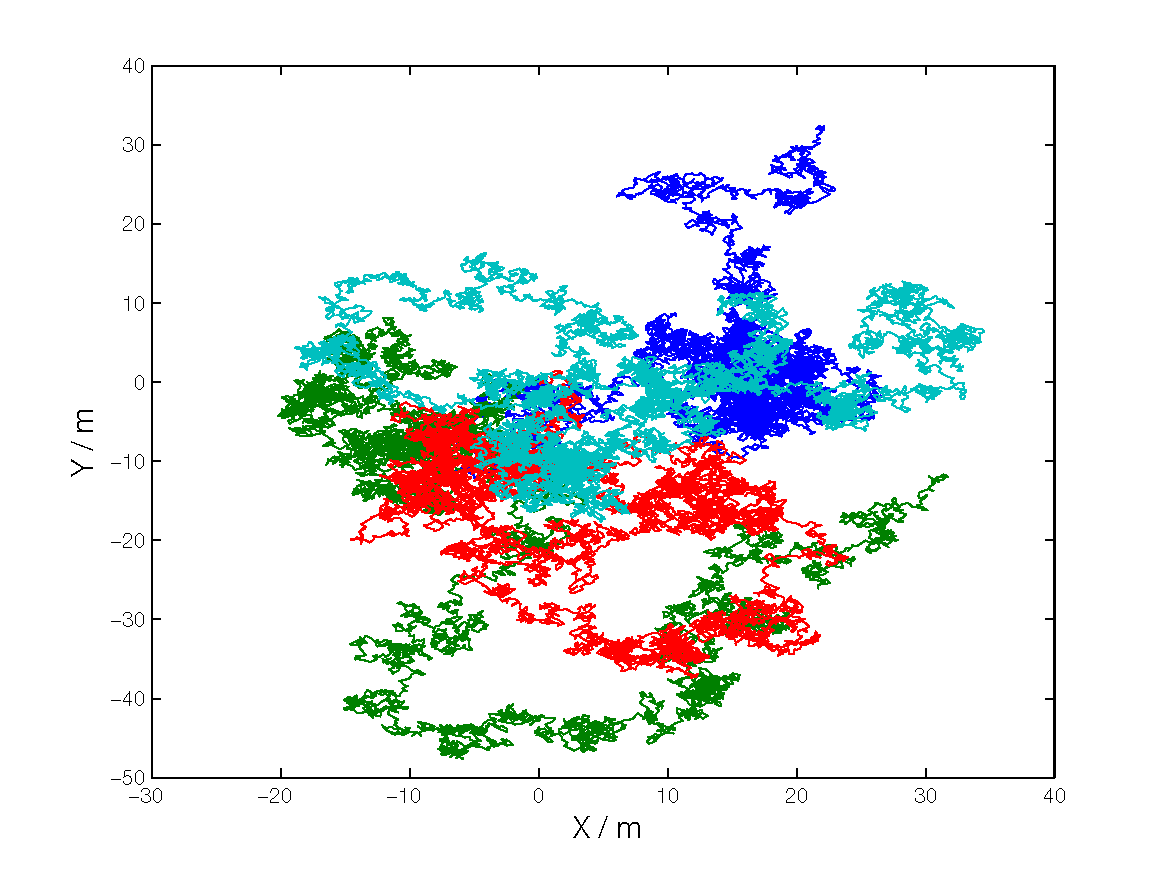
\includegraphics[width=1\textwidth ]{images/kinematic/rand_walk}
\caption{Four series of random walk using $\sigma = 1$ and $10000$ steps.}\label{rand_walk}
\end{figure}
%
\section{Quaternions}
%
The \emph{quaternions} are an extension of the complex numbers, first described in 1843 by the Irish mathematician William Rowan Hamilton. They were first used in three-dimensional mechanics and today they are, among other applications, used to estimate the pose (position and direction in relation to a fixed frame) in three dimensions \cite{mann13}.
%
\subsection{Quaternion Theory}
%
As stated before a quaternion, $q$, is a set of numbers, extending the complex numbers, defined as
%
\begin{equation}
q = a+bi+cj+dk, \hspace{5pt}[a,b,c,d]\in \mathbb R
\end{equation} 
%
where \emph{i, j} and $k$ are new basis elements.

Further, the basis elements obey
%
\begin{equation}
\label{equation:basis}
i^2=j^2=k^2=ijk=-1
\end{equation}
%
Thus, from \ref{equation:basis} all possible of the basis multiplications can be formed according to Table \ref{table:basis}.
%
\begin{table}[!hbt]
\begin{center}
\begin{tabular}{|c|c|c|c|c|}
\hline
$\times$ & $1$ & $i$ & $j$ & $k$ \\
\hline
$1$ & $1$ & $i$ & $j$ & $k$ \\
\hline 
$i$ & $i$ & $-1$ & $k$ & $-j$\\
\hline
$j$ & $j$ & $-k$ & $-1$ & $i$ \\
\hline
$k$ & $k$ & $j$ & $-i$ & $-1$ \\
\hline
\end{tabular}
\end{center}
\caption{All possible basis multiplications for quaternions.}
\label{table:basis}
\end{table}
%
A quaternion is usually seen as a four-dimensional vector consisting of a scalar $q_0$ and a vector $\vec{q} = (q_1 \; \; q_2 \; \; q_3)^T$, leading to the following notation
%
\begin{equation}
q = \left(\begin{array}{c}q_0\\ \vec{q}\end{array}\right) = \left(\begin{array}{c}q_0\\ q_1 \\ q_2 \\ q_3\end{array}\right). 
\end{equation}  
%
Quaternion multiplication is denoted by $\otimes$ and defined 
%
\begin{equation}
q\otimes r = \left(\begin{array}{c}q_0\\ \vec{q}\end{array}\right) \otimes \left(\begin{array}{c}r_0\\ \vec{r}\end{array}\right) =
\left(\begin{array}{c}q_0r_0-\vec{q} \cdot \vec{r}\\ q_0\vec{r}+r_0\vec{q}+\vec{q}\times \vec{r}\end{array}\right)
\end{equation}
%
for two quaternions $q$ and $r$, where $\cdot$ denote the scalar product and $\times$ denote the vector product. The quaternion multiplication is non-commutative, meaning
%
\begin{equation}
{q}\otimes {r} \neq {r} \otimes {q}
\end{equation}
%
in general. It is, however associative
%
\begin{equation}
({q}\otimes{r})\otimes{s} = {q}\otimes({r}\otimes{s}).
\label{equation:quat_asso}
\end{equation} 
%
Further, the \emph{unit} quaternion is defined as
%
\begin{equation}
{q_{\mathbf{I}}}=\left(\begin{array}{c}1\\ 0 \\ 0 \\ 0\end{array}\right)
\end{equation}
%
and the quaternion inverse $q^{-1}$ is
%
\begin{eqnarray}
q^{-1}\otimes q = q\otimes q^{-1} = q_{\mathbf{I}} &\Leftrightarrow& q^{-1} = \frac{1}{|q|^2}\left(\begin{array}{c}q_0\\ -\vec{q}\end{array}\right)
\end{eqnarray}
%
where the quaternion norm $|q|$ is defined as
%
\begin{equation}
|q| = \sqrt{q_0^2+q_1^2+q_2^2+q_3^2 }.
\end{equation} 
%
\subsection{Quaternions Interpreted as Rotations}
%
Why a certain subset of quaternions, $|q|=1$ may be interpreted as rotations is beyond the scope of this thesis. Instead, here follows a recapitulation of how they can be uses. Reader interested in the mechanisms involved are referred to \cite{kuip98} for an in-depth discussion of the background and theory of quaternions. 

Rotations are defined by two elements, the amount (angle) of rotation and around what axis the rotation is performed. Suppose that a rotation of $\theta$ is performed around the three-dimensional unit vector $\vec n$. The quaternion representation of this would be
\begin{equation}
q = \left(\begin{array}{c}\cos{\frac{\theta}{2}}\vspace{5pt}\\ \vec{n}\sin{\frac{\theta}{2}}\end{array}\right).
\end{equation}  
%
Finding the vector $\vec v$ rotated clockwise by $\theta$ around $\vec n$, noted $\vec v_r$, by use of quaternions is done as
%
\begin{equation}
\left(\begin{array}{c}0\\ \vec{v_r}\end{array}\right) = q\otimes \left(\begin{array}{c}0\\ \vec{v}\end{array}\right) \otimes q^{-1}.
\end{equation}
%
From here on, the naming convention
%
\begin{equation}
\vec v\equiv \left(\begin{array}{c}0\\ \vec{v}\end{array}\right).
\end{equation}
%
The rotation of a vector, $\vec v$, by a quaternion, $q$ and subsequently by $p$ is equivalent to rotating $\vec v$, by the corresponding quaternion product $(p\otimes q)$. This is easily proven by multiple applications of \ref{equation:quat_asso},
%
\begin{equation}
(p\otimes q)\otimes \vec v \otimes (p\otimes q)^{-1}=p\otimes(q\otimes\vec v\otimes q^{-1})\otimes p^{-1}. 
\end{equation}
%
When using sensors, in particular a gyroscope, to compute the rotation, it is common to end up with integrated angular velocities on the form $\vec{r} = (r_x \; \; r_y \; \; r_z)^T$. Each element in $\vec r$ characterize the rotation around an axis in an orthogonal coordinate system, in a relatively short timespan. To describe this rotation using quaternions, the direction around which the rotation is performed can be viewed as the direction of $\vec r$, and the vector norm $|\vec r|$ may be considered the angle of rotation. The corresponding quaternion, $q$, is then
%
\begin{equation}
q = \left(\begin{array}{c}\cos{\frac{|\vec r|}{2}}\vspace{5pt} \\ \frac{\vec{r}}{|\vec r|}\cos{\frac{|\vec r|}{2}}\end{array}\right)
\end{equation}
%
\section{Characterization of Steps}
%
Characterizing a step allows a kinematics algorithm to keep track of the approximate distance travelled, as the length of a particular individuals steps is relatively regular. A way to identify whether a step has been taken, could be constructed using an accelerometer \cite{step_count}. As stated earlier the accelerometer gives output on the form $\vec a = (a_x \hspace{5pt} a_y \hspace{5pt} a_z)^T$, each element representing the acceleration along each of the phones  coordinate axis. However, the orientation of the phone during a walk affects how each element in the acceleration vector behaves, a phone placed in a pocket or a bag give vastly different output. A more robust way is to consider the average acceleration ,$|\vec a|$, defined in unison with the vector norm as 
%
\begin{equation}
|\vec a| = \sqrt{a_x^2+a_y^2+a_z^2},
\end{equation}
%
which is considerably more similar between use cases.
%
\begin{figure}[!hbt]
\include{graphics}
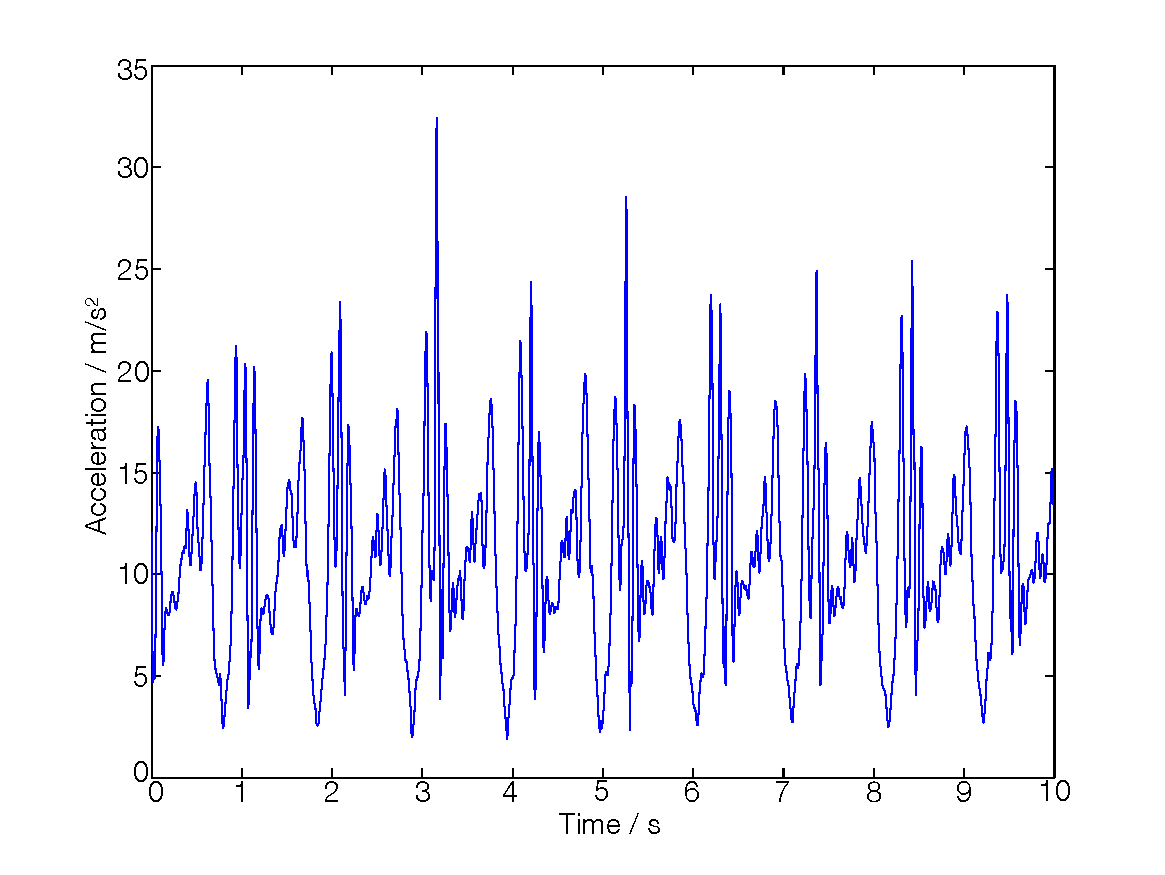
\includegraphics[width=1\textwidth ]{images/kinematic/avr_acc}
\caption{Average acceleration during 10 seconds of a typical walk.}\label{avr_acc}
\end{figure}

A 10 second sample of the average acceleration measured by a phone placed in the front pocket during a typical walk is displayed in Figure \ref{avr_acc}. A flaw of this approach is easily noticed. Due to gravity, the average acceleration is centered around this value, ($9.81$ m/s$^2$). A way around this is to differentiate the signal according to 
%
\begin{equation}
\Delta f(x) = \frac{f(x+\Delta t) - f(x) }{\Delta t},
\end{equation} 
%
\begin{figure}[!hbt]
\include{graphics}
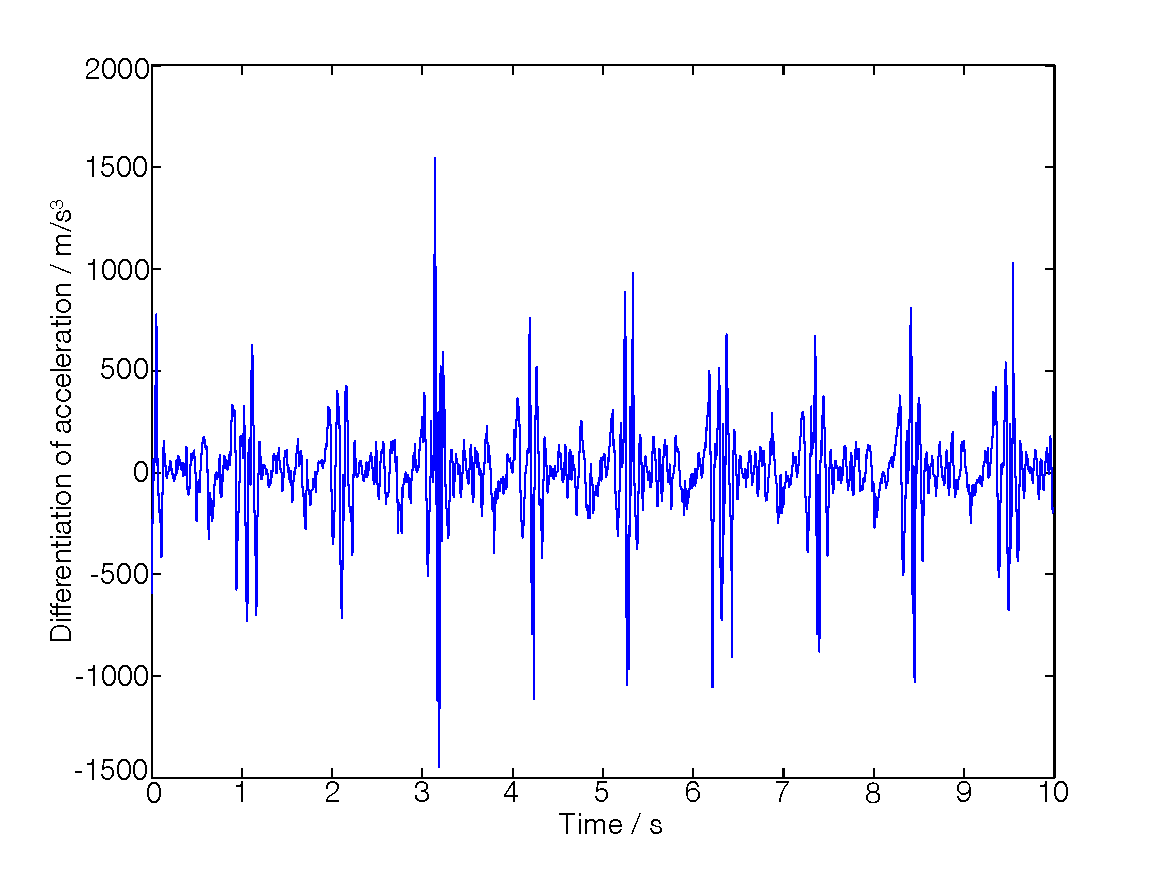
\includegraphics[width=1\textwidth ]{images/kinematic/avr_acc_dif}
\caption{Differentiation of average acceleration during 10 seconds of a typical walk.}\label{avr_acc_dif}
\end{figure}
%
yielding a signal according to Figure \ref{avr_acc_dif}. This signal is centred around zero, but possesses unnecessary high frequency behaviour. The sampling frequency of the accelerometer is $\sim 20$ Hz, giving a frequency content of the signal between 0 and 10 Hz. The normal step frequency for a person is no larger than 3 Hz, which promotes filtering the signal. Doing this with a fourth order \emph{Butterworth filter} with a cut-of frequency of 3 Hz yields the signal in Figure \ref{avr_acc_dif_filt} \cite{pro07}.
%
\begin{figure}[!hbt]
\include{graphics}
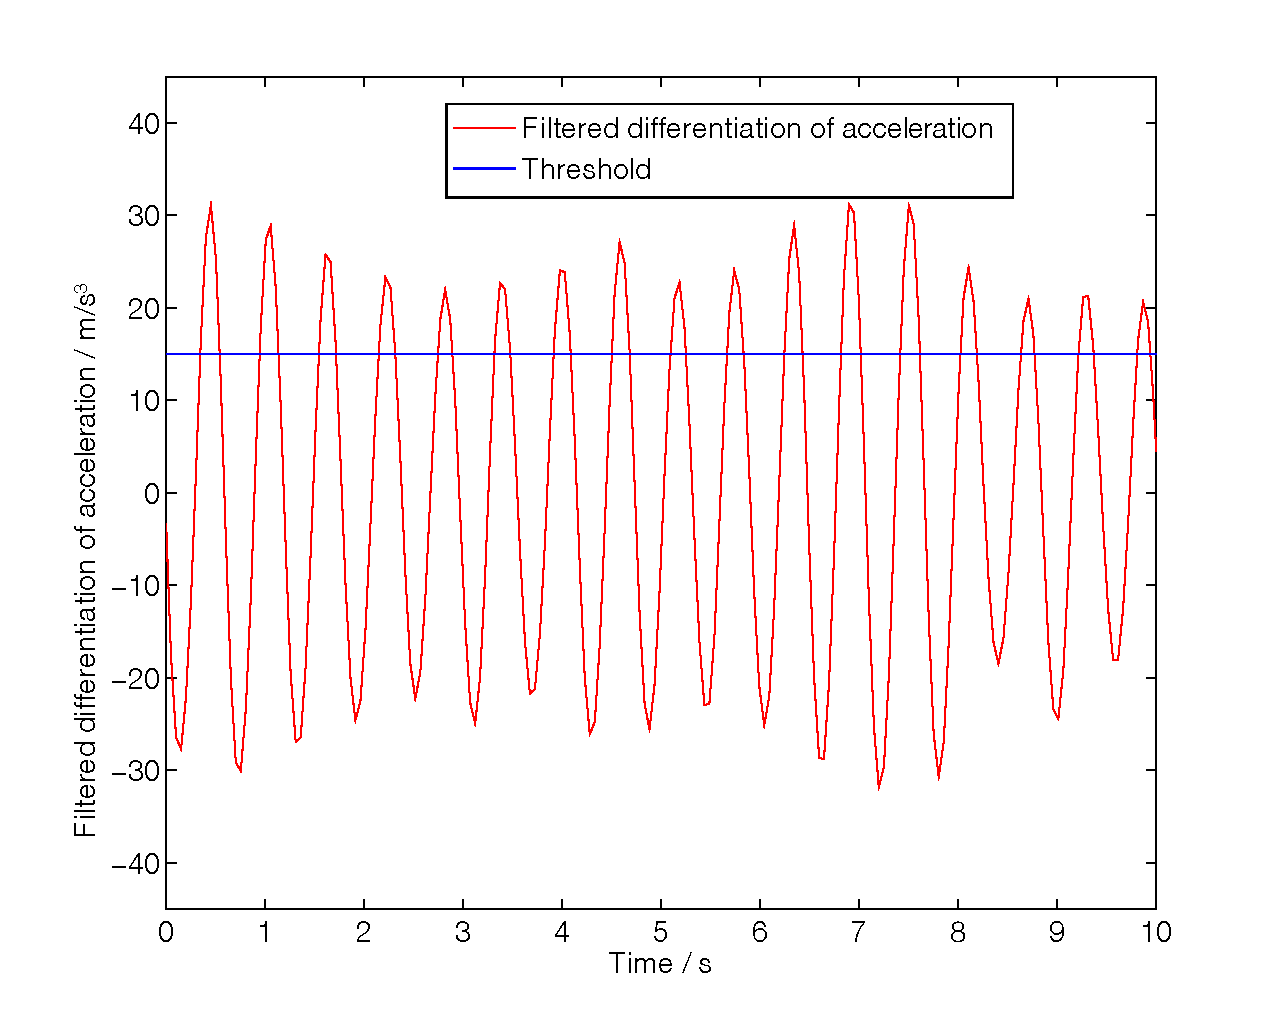
\includegraphics[width=1\textwidth ]{images/kinematic/avr_acc_dif_filt}
\caption{Filtered differentiation of average acceleration during 10 seconds of a typical walk with phone carried in hand (Red) and threshold to determine in step has been taken (blue). }\label{avr_acc_dif_filt}
\end{figure}
%
Here, the steps are clearly distinguishable and each peaks corresponds to a step taken. In Figure \ref{avr_acc_dif_filt} a threshold for determining weather a step has been taken or not is also present. A simple rule to count the number of steps taken could be to count the number of times the signal passes from below to above the threshold. Using this rule 17 steps was taken during the 10 second interval displayed in Figure \ref{avr_acc_dif_filt}.

A algorithm corresponding to the rule above has been implemented in android using java. To test the performance of the algorithm two walks of 100 steps respectively was made, one with the phone in hand and one with the phone in the front right jeans pocket. When the phone was carried in hand 101 steps was registered and when carried in pocket 
100 steps was registered. This shows the simple algorithm producing satisfactory results in these common use cases.
The technique could be refined further, by e. g identifying the step frequency or by using more sensors. However, the performance in this for is sufficient for the application it is intended for.  
%
\subsection{Step Length Considerations}
%
The step length of an individual, moving in a straight line with a constant speed, is more or less constant. Different individuals or the same individual moving at different speeds or performing turns have a quite large span of step lengths. In this thesis the step length has been determined by the authors walking a predetermined distance comprised of walking straight interspersed with turning both left and right, at a constant speed. The average step length is then simply computed as the distance divided by number of steps and a value of $0.77$ meters was obtained.  

For real world usage however, the length of a user's steps must be determined. This can be done in various ways, one is to have the user estimate their own step length with the same method as above. Another is to adaptively tune the step length by using approximately known distances travelled and the number of steps taken whilst traveling. A way of doing this is to use some sort of positioning technique (GPS, WiFi etc.) to estimate the distance while the step counter determines the number of steps.

An alternative method is to add step length as a state in the particle filter corresponding to step length and spread the particles according to their step length. Particles with to long or to short step length would agree badly with measured RSSI-values and thus be given a small weight. A downside to this is that increasing the number of states would require more particles as discussed in section \ref{sec:nlfp} consequently increasing the computational power required to implement the filter.      
%
\section{Direction of Movement}
%
To have a good estimation of the movement, not only the distance travelled needs to be known. More importantly is the direction in which the movement takes place. In addition, this task is more complicated than finding the distance by the number of steps taken. Many approaches are available using a wide span of technologies. 
%
\subsection{Integrated gyroscope}
%

%
\subsection{Sensor Fused Approaches}
%
There are different approaches for combining magnetometer, gyroscope and possibly other sensors to produce a sensor fused estimation of the heading. Most Android phones implement such an algorithm, using gyroscope, magnetometer and accelerometer to produce an estimate of how the phone is oriented in the world coordinate system. The algorithm uses gyroscope and accelerometer to determine when the magnetometer output is corrupted, and uses their measurements to estimate the heading until the magnetometer can be trusted. 
%
\subsection{Direction as a Particle Filter State}
%
Another method for estimating the direction of movement is to extend the 
%
\section{Dead Reckoning}
%
\emph{Dead reckoning} is the process of calculating the current position based on a previously determined position and advancing that position based on a known model. Dead reckoning has been used by e. g ships and airplanes for a long time, and in more resent time in networked computer games. 

Dead reckoning estimations are subject to cumulative errors i.e. errors are added over time and depending on the accuracy of the dead reckoning system, the estimated position deviates from the true. This implies that the position and heading estimates need to be calibrated at a certain time interval to provide an accurate position.

For phones, a dead reckoning estimation would most likely include some form of step counting combined with one of the heading estimations previously mentioned. As an example, the true and estimated paths using a pedometer and a gyroscope during a walk of approximately 110 meters, are presented in Figure \ref{deadreckon_1}. The behavior is fairly good but there is a heading error present soon after the start, and this grows as the walk continues. The distance estimated by the pedometer is also larger than the true distance traveled.  
%
\begin{figure}[!hbt]
\include{graphics}
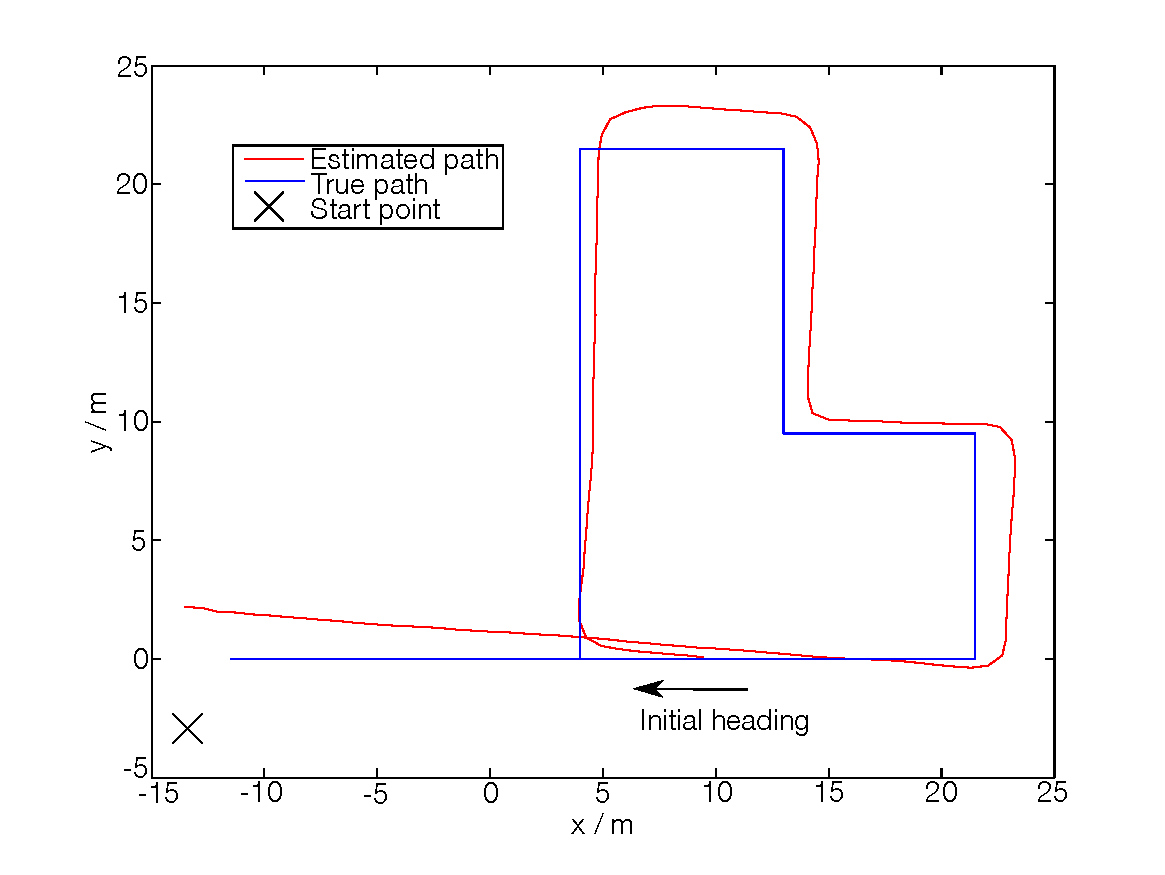
\includegraphics[width=1\textwidth ]{images/kinematic/deadreckon_1}
\caption{True versus, by dead reckoning, estimated path using gyroscope and pedometer.}\label{deadreckon_1}
\end{figure}

However, as stated before, the error is cumulative and the performance deteriorates with time. This is shown in Figure \ref{deadreckon_2}. The distance around the rectangle is approximately 105 meters, and especially the heading error is clearly visible. 
%
\begin{figure}[!hbt]
\include{graphics}
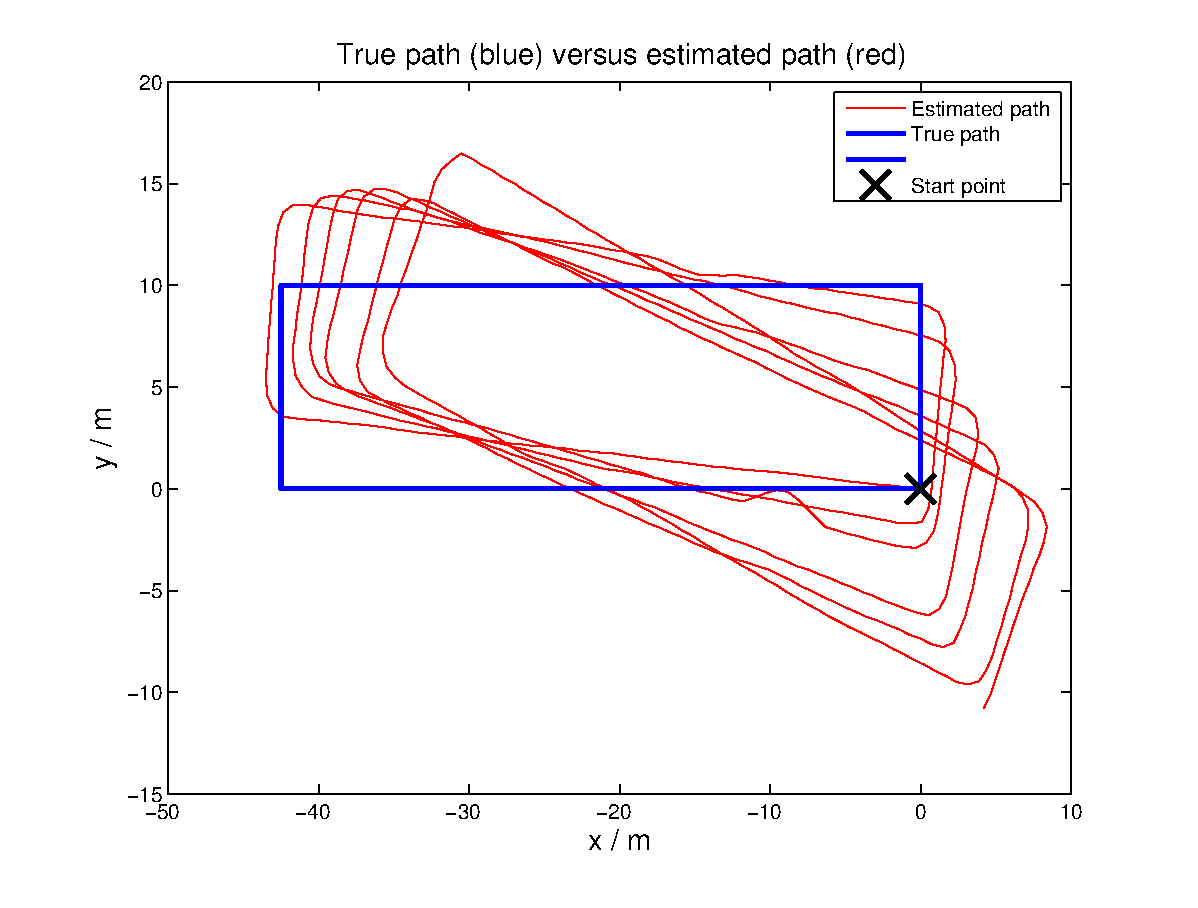
\includegraphics[width=1\textwidth ]{images/kinematic/deadreckon_2}
\caption{True versus, by dead reckoning, estimated path using gyroscope and pedometer.}\label{deadreckon_2}
\end{figure}

It is apparent that both position and heading need to be calibrated to obtain a good position estimate. How this is done is explained in the following chapters.
%
\chapter{Indoor positioning - Sensor Fused Approach} 
%
\chapter{Algorithm Implementation in Android}
%
In previous chapters offline computations are used to obtain the position estimate. Here an online java implementation of the developed algorithms will be presented briefly. The particle filter is quite computationally demanding, and therefor it is important to discern if handheld devices are capable of performing these computations sufficiently fast. 

The implementation will be done in a positioning application developed by Sony Mobile, called SonyMap \cite{sonymap}. This application is intended for android smartphones and used to navigate and position the smartphone in Sony Mobiles buildings around the globe. 

The chapter is closed by discussing some further optimizations possible, if it is necessary to decrease the computational time further.  
%
\subsection{Introducing SonyMap}
%
\section{Choice of Coordinate System}
%
\section{Java Implementations}
%
\subsection{Finding Building \& Floor}
%
\subsection{The Particle Filter}
%
\section{Further Optimizations - Parallel Computations}
%


The sensors described in the (previous chapter) provide additional information for the positioning. The gyroscope indicates  if the user has changed direction, and how much, while the step counter provides an estimation of how far the user has moved since the last time step.

One way to use the information from the gyroscope is to introduce the direction of movement as a new state of each particle. Initially, each particle is given a uniformly random direction in the interval $[0,2 \pi)$. 

\printbibliography  %% Comment if you don't want to use bibtex

\end{document}





